\documentclass{beamer}
\usepackage[utf8]{inputenc}
\usepackage[english,russian]{babel}
\usepackage{amsmath}
\usepackage{amsthm}
\usepackage{amssymb}
\usepackage{fancyhdr}
\usepackage{setspace}
\usepackage{graphicx}
\usepackage{colortbl}
\usepackage{tikz}
\usepackage{pgf}
\usepackage{subcaption}
\usepackage{listings}
\usepackage{indentfirst}
\usepackage{csquotes}
\usepackage{pgfpages}

\setbeamertemplate{navigation symbols}{}
\setbeameroption{show notes on second screen}
\setbeamertemplate{note page}[plain]
\setbeamerfont{note page}{size=\tiny}

\mode<presentation> {
	\usetheme{Boadilla}
	\usecolortheme{lily}
}

\usefonttheme{serif}

\usepackage[sorting=nyt, backend=bibtex]{biblatex}
\addbibresource{bibliography.bib}

%----------------------------------------------------------------------------------------
%	TITLE PAGE
%----------------------------------------------------------------------------------------

\title[Атаки на мультиязычные модели]{Выпускная квалификационная работа\\``Атаки на мультиязычные модели''}

\author[Алексей Биршерт 171]{
	Биршерт Алексей Дмитриевич БПМИ 171 \\
	\bigskip
	Руководитель ВКР: Артемова Екатерина Леонидовна
}
\date{\today}

\begin{document}

	\begin{frame}
		\titlepage

		\note{Добрый день, уважаемая комиссия. Меня зовут Алексей Биршерт и сегодня я представляю Вам свою выпускную квалификационную работу под названием “Атаки на мультиязычные модели”, которую я выполнял под научным руководством Екатерины Артемовой.}
	\end{frame}

%------------------------------------------------


	\section{Введение}
%------------------------------------------------

	\begin{frame}{Смешение кодов}
		\begin{figure}[c]
			\centering
			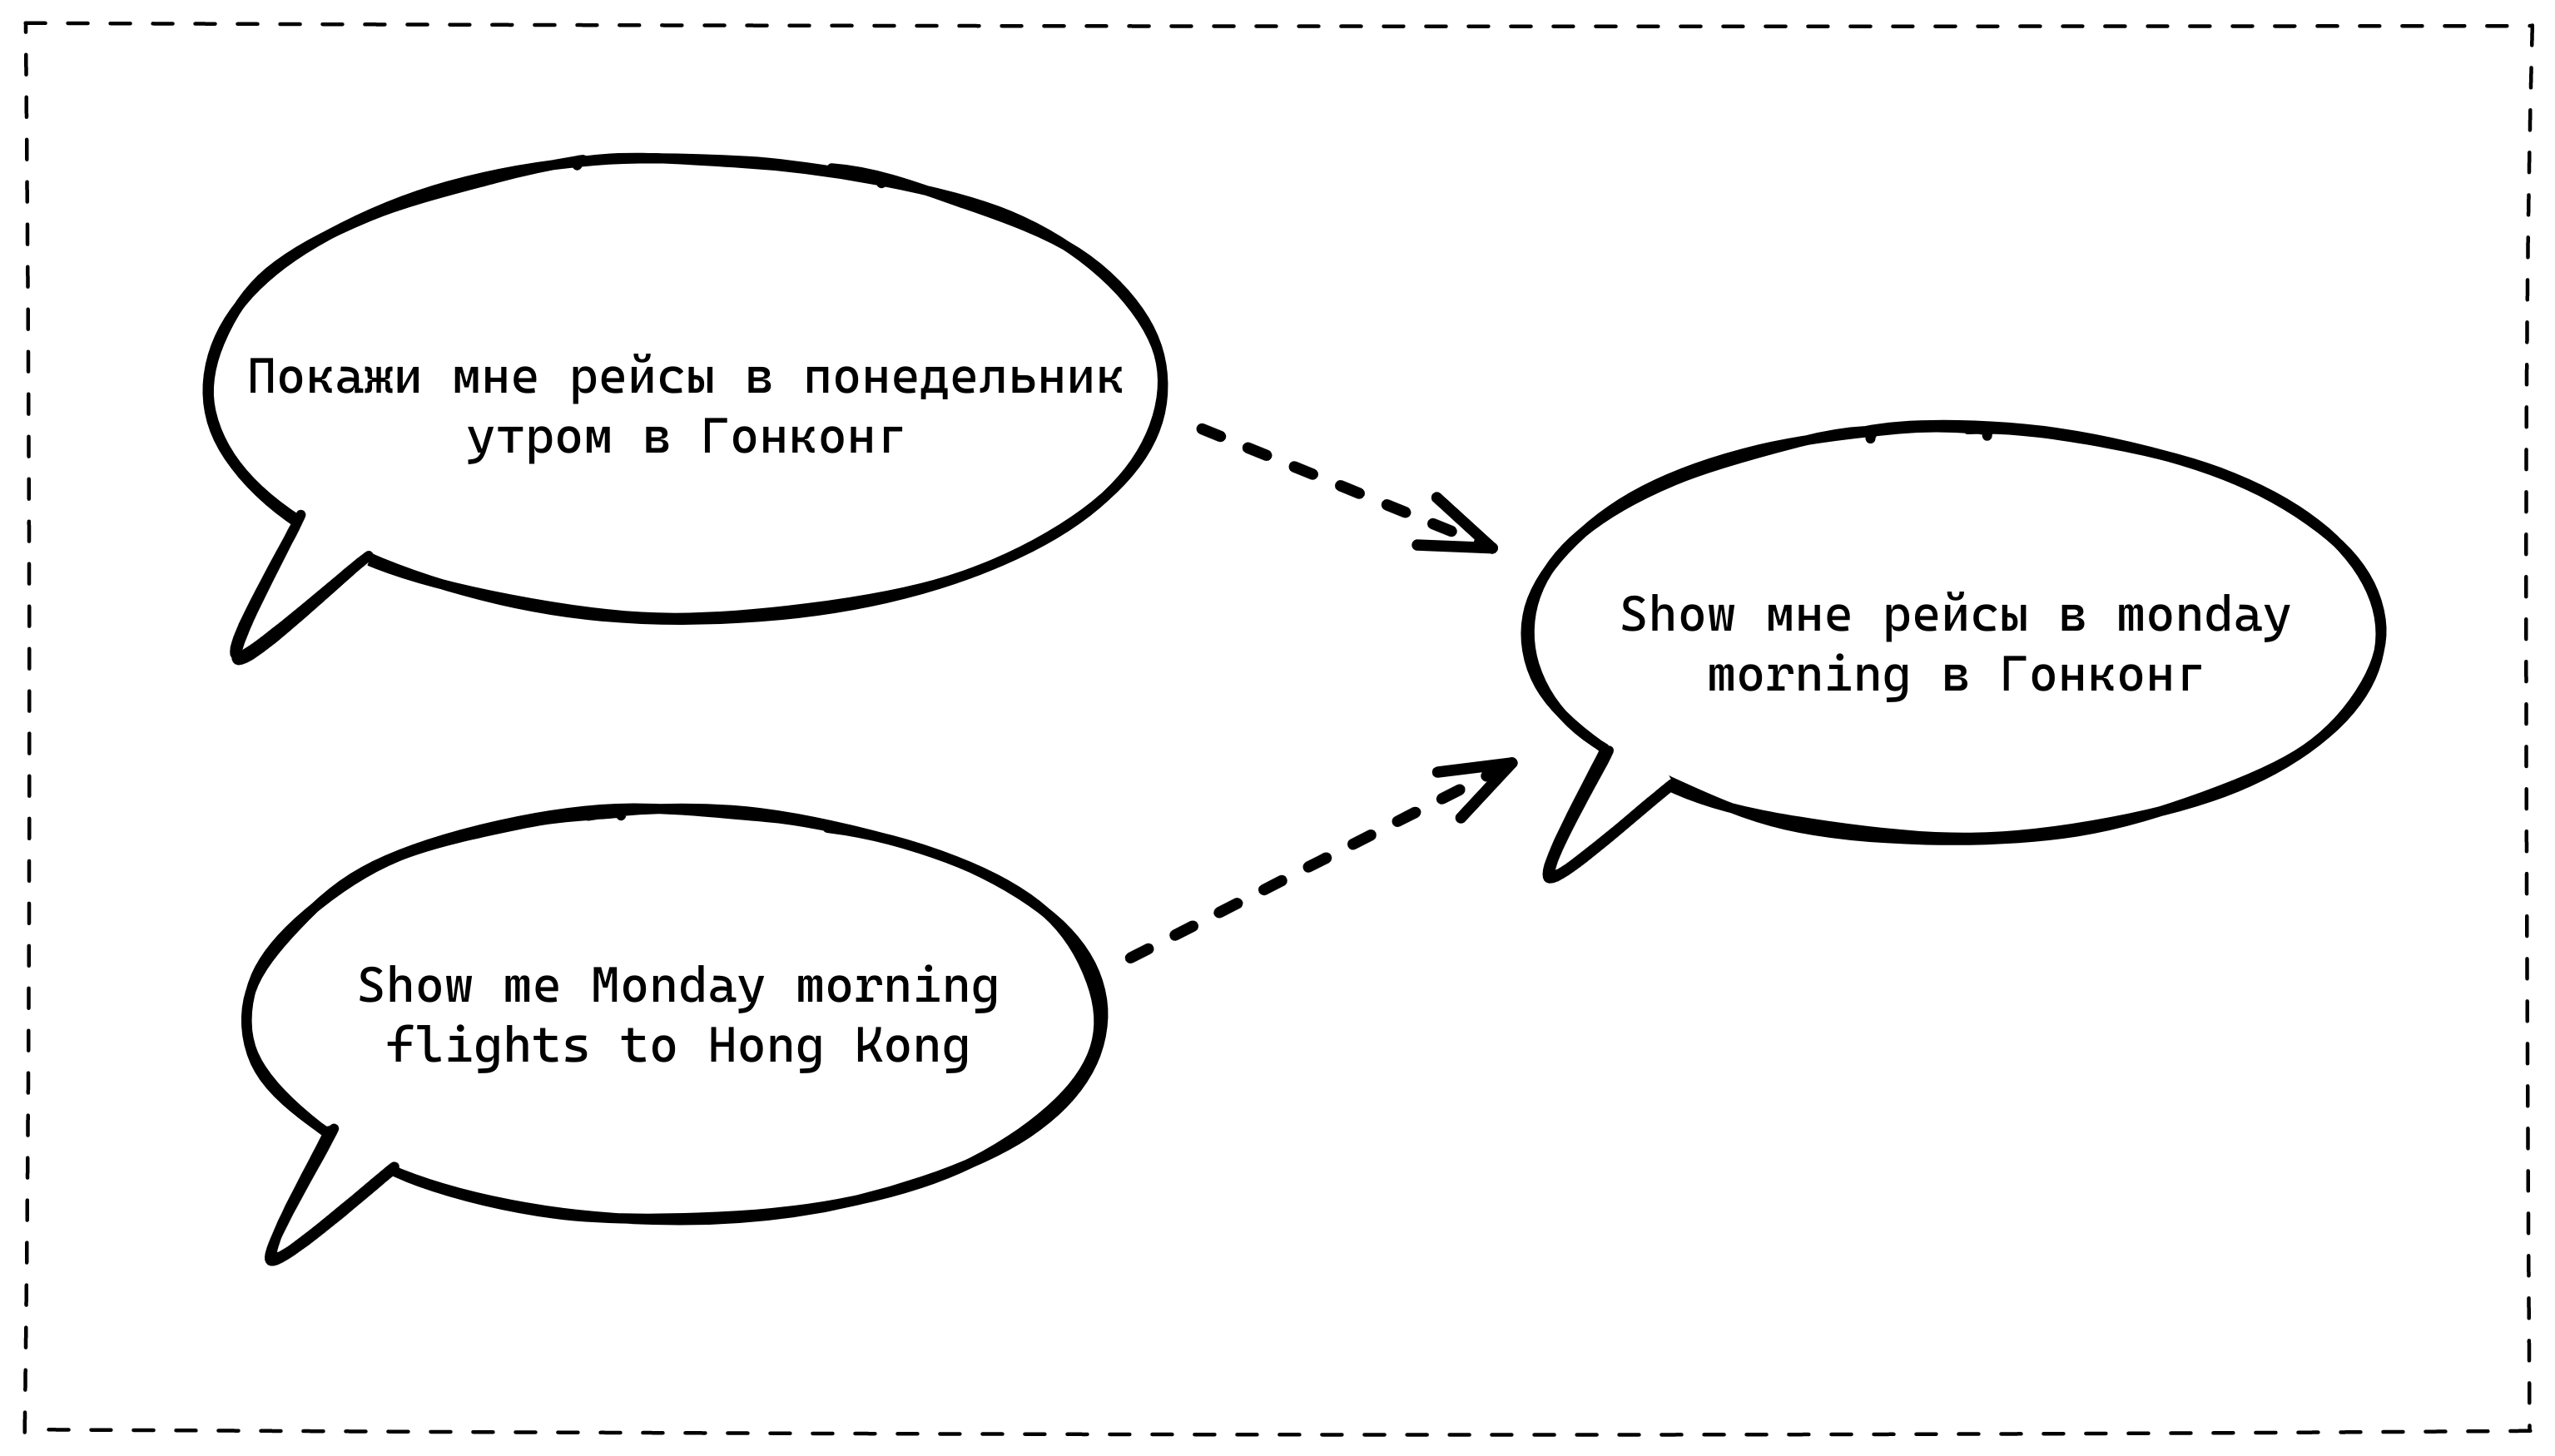
\includegraphics[width=\linewidth]{slides/1}\label{fig:figure}
		\end{figure}

		\note{В мультиязычных сообществах по всему миру распространен такой феномен как смешение кодов. Смешение кодов — это процесс, когда человек смешивает различные языки внутри одной фразы или предложения. Это может происходить как в устной, так и в письменной речи. Несмотря на то, что реальные данные со смешением кодов существуют, эти данные очень дорогие и в сборе и в разметке.}
	\end{frame}

	\begin{frame}{Имитация смешения кодов}
		\begin{itemize}
			\item Хотим оценить качество моделей на смешении кодов
			\item Данных со смешением кодов мало
			\item Качество после атак как нижняя оценка
		\end{itemize}

		\note{В своей работе мы оцениваем качество мультиязычных моделей на входных данных со смешением кодов. В силу отсутствия большого количества таких данных, мы оцениваем это качество с помощью атак, которые имитируют смешение кодов. Мы предполагаем, что качество после таких атак будет являться нижней оценкой на реальное качество. Для смешения кодов было показано, что если модель успешно справляется с искусственными примерами, полученными после атак, то она будет как минимум не хуже справляться с реальными данными. Таким образом, в своей работе мы предложили две атаки, которые имитируют смешение кодов и также мы придумали метод защиты от таких атак, который позволяет увеличить качество на данных со смешением кодов.\newlineНаша работа является одной из первых работ этой области. Актуальность темы подтверждается наличием двух статей на данную тему, которые были опубликованы в международных рецензируемых журналах в середине марта текущего года.}
	\end{frame}

%------------------------------------------------


	\section{Постановка задачи}
%------------------------------------------------

	\begin{frame}{Постановка задачи}
		\begin{onlyenv}<1>
			\begin{figure}
				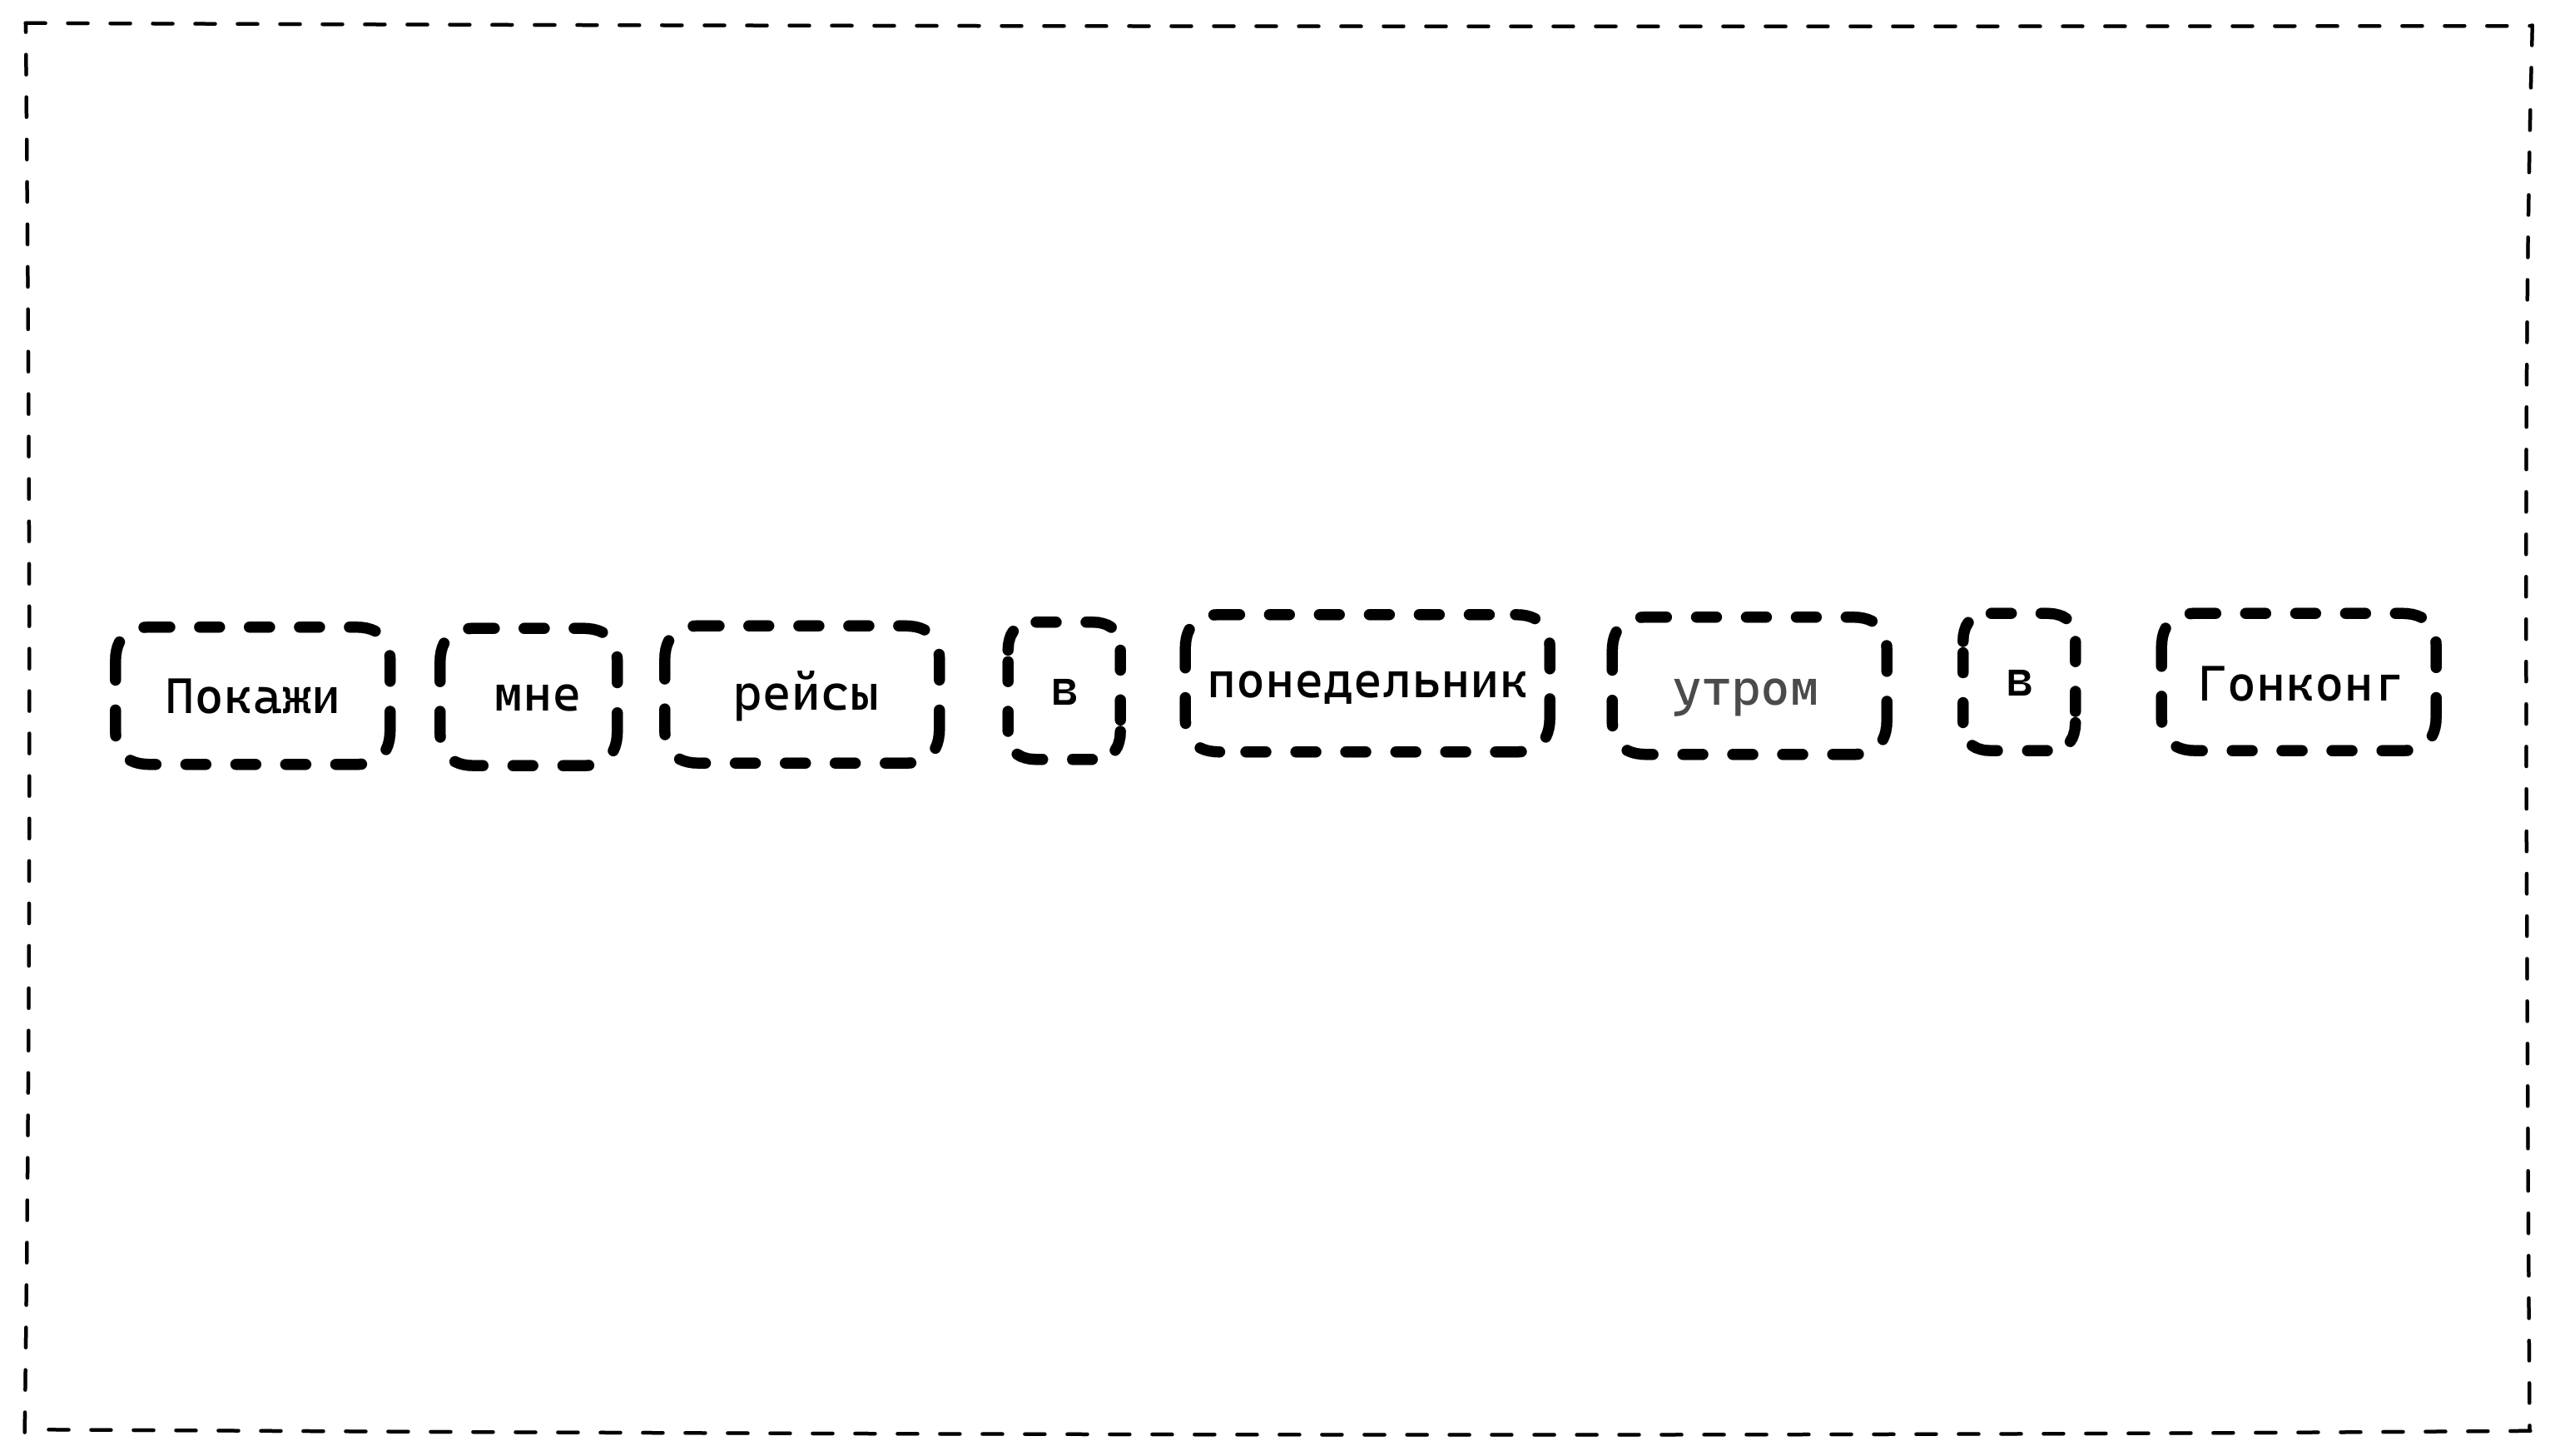
\includegraphics[width=\linewidth]{slides/2}\label{fig:figure2}
			\end{figure}
		\end{onlyenv}

		\begin{onlyenv}<2>
			\begin{figure}
				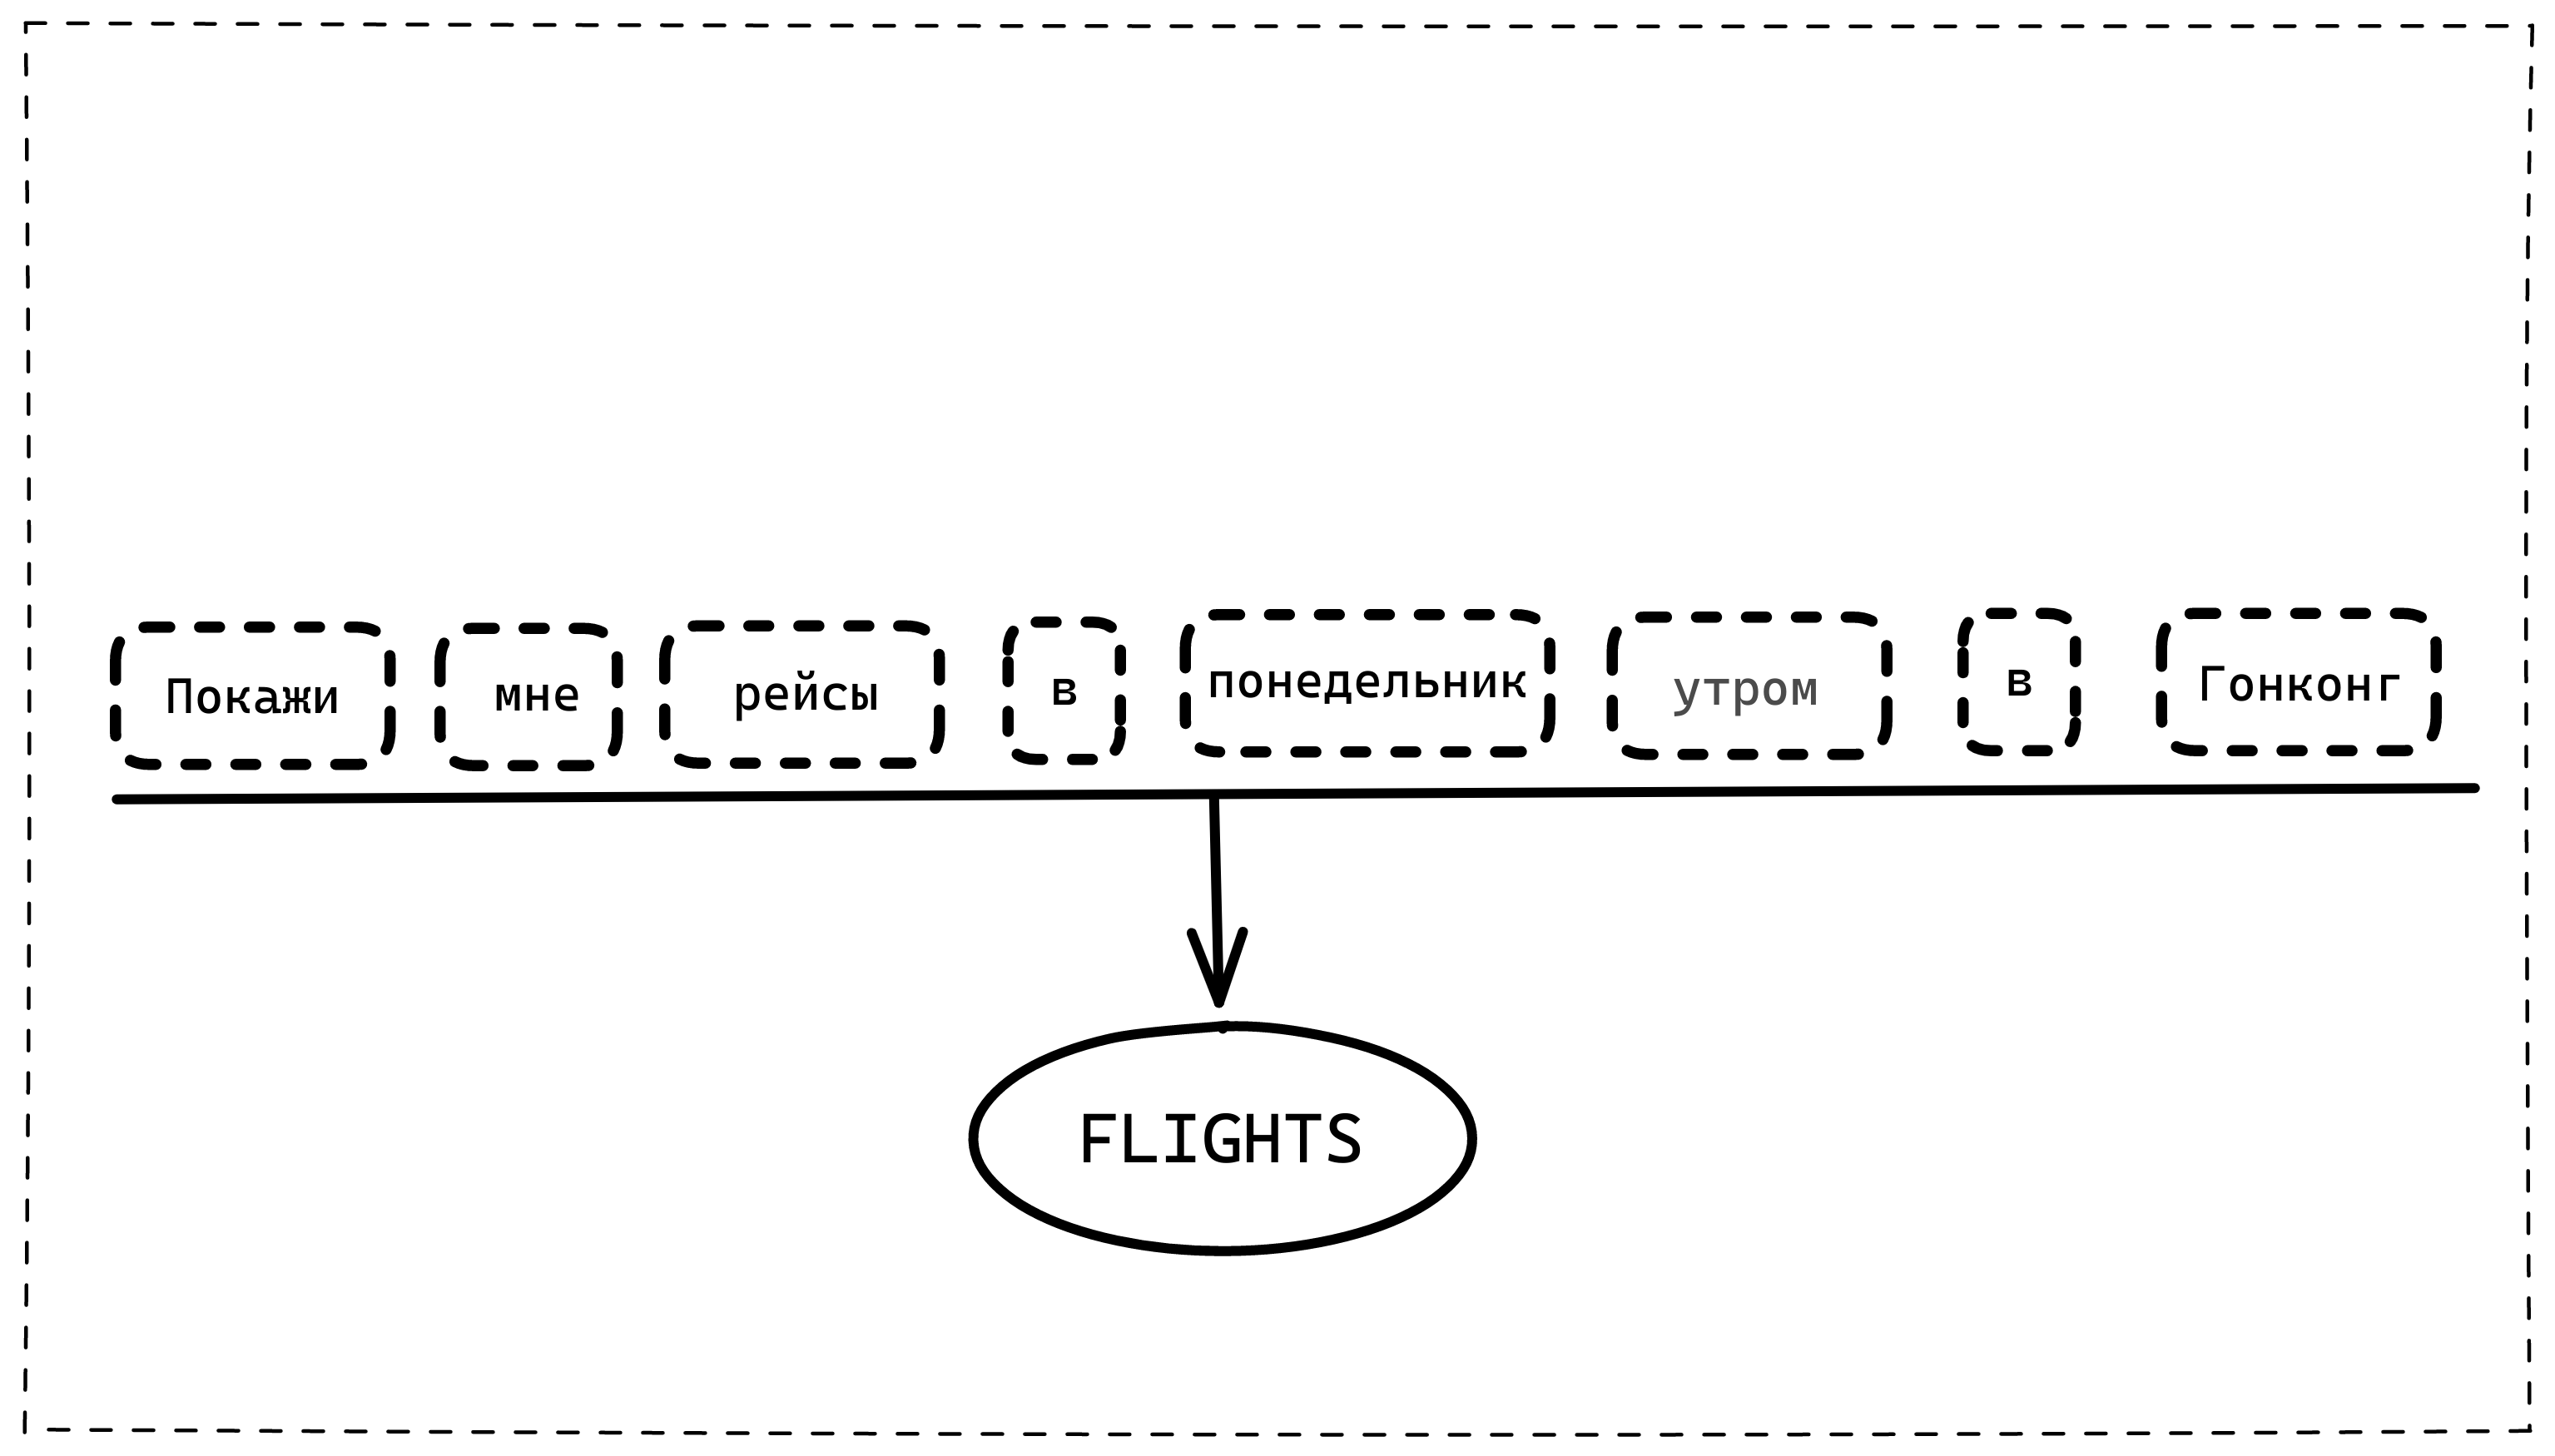
\includegraphics[width=\linewidth]{slides/3}\label{fig:figure3}
			\end{figure}
		\end{onlyenv}

		\begin{onlyenv}<3>
			\begin{figure}
				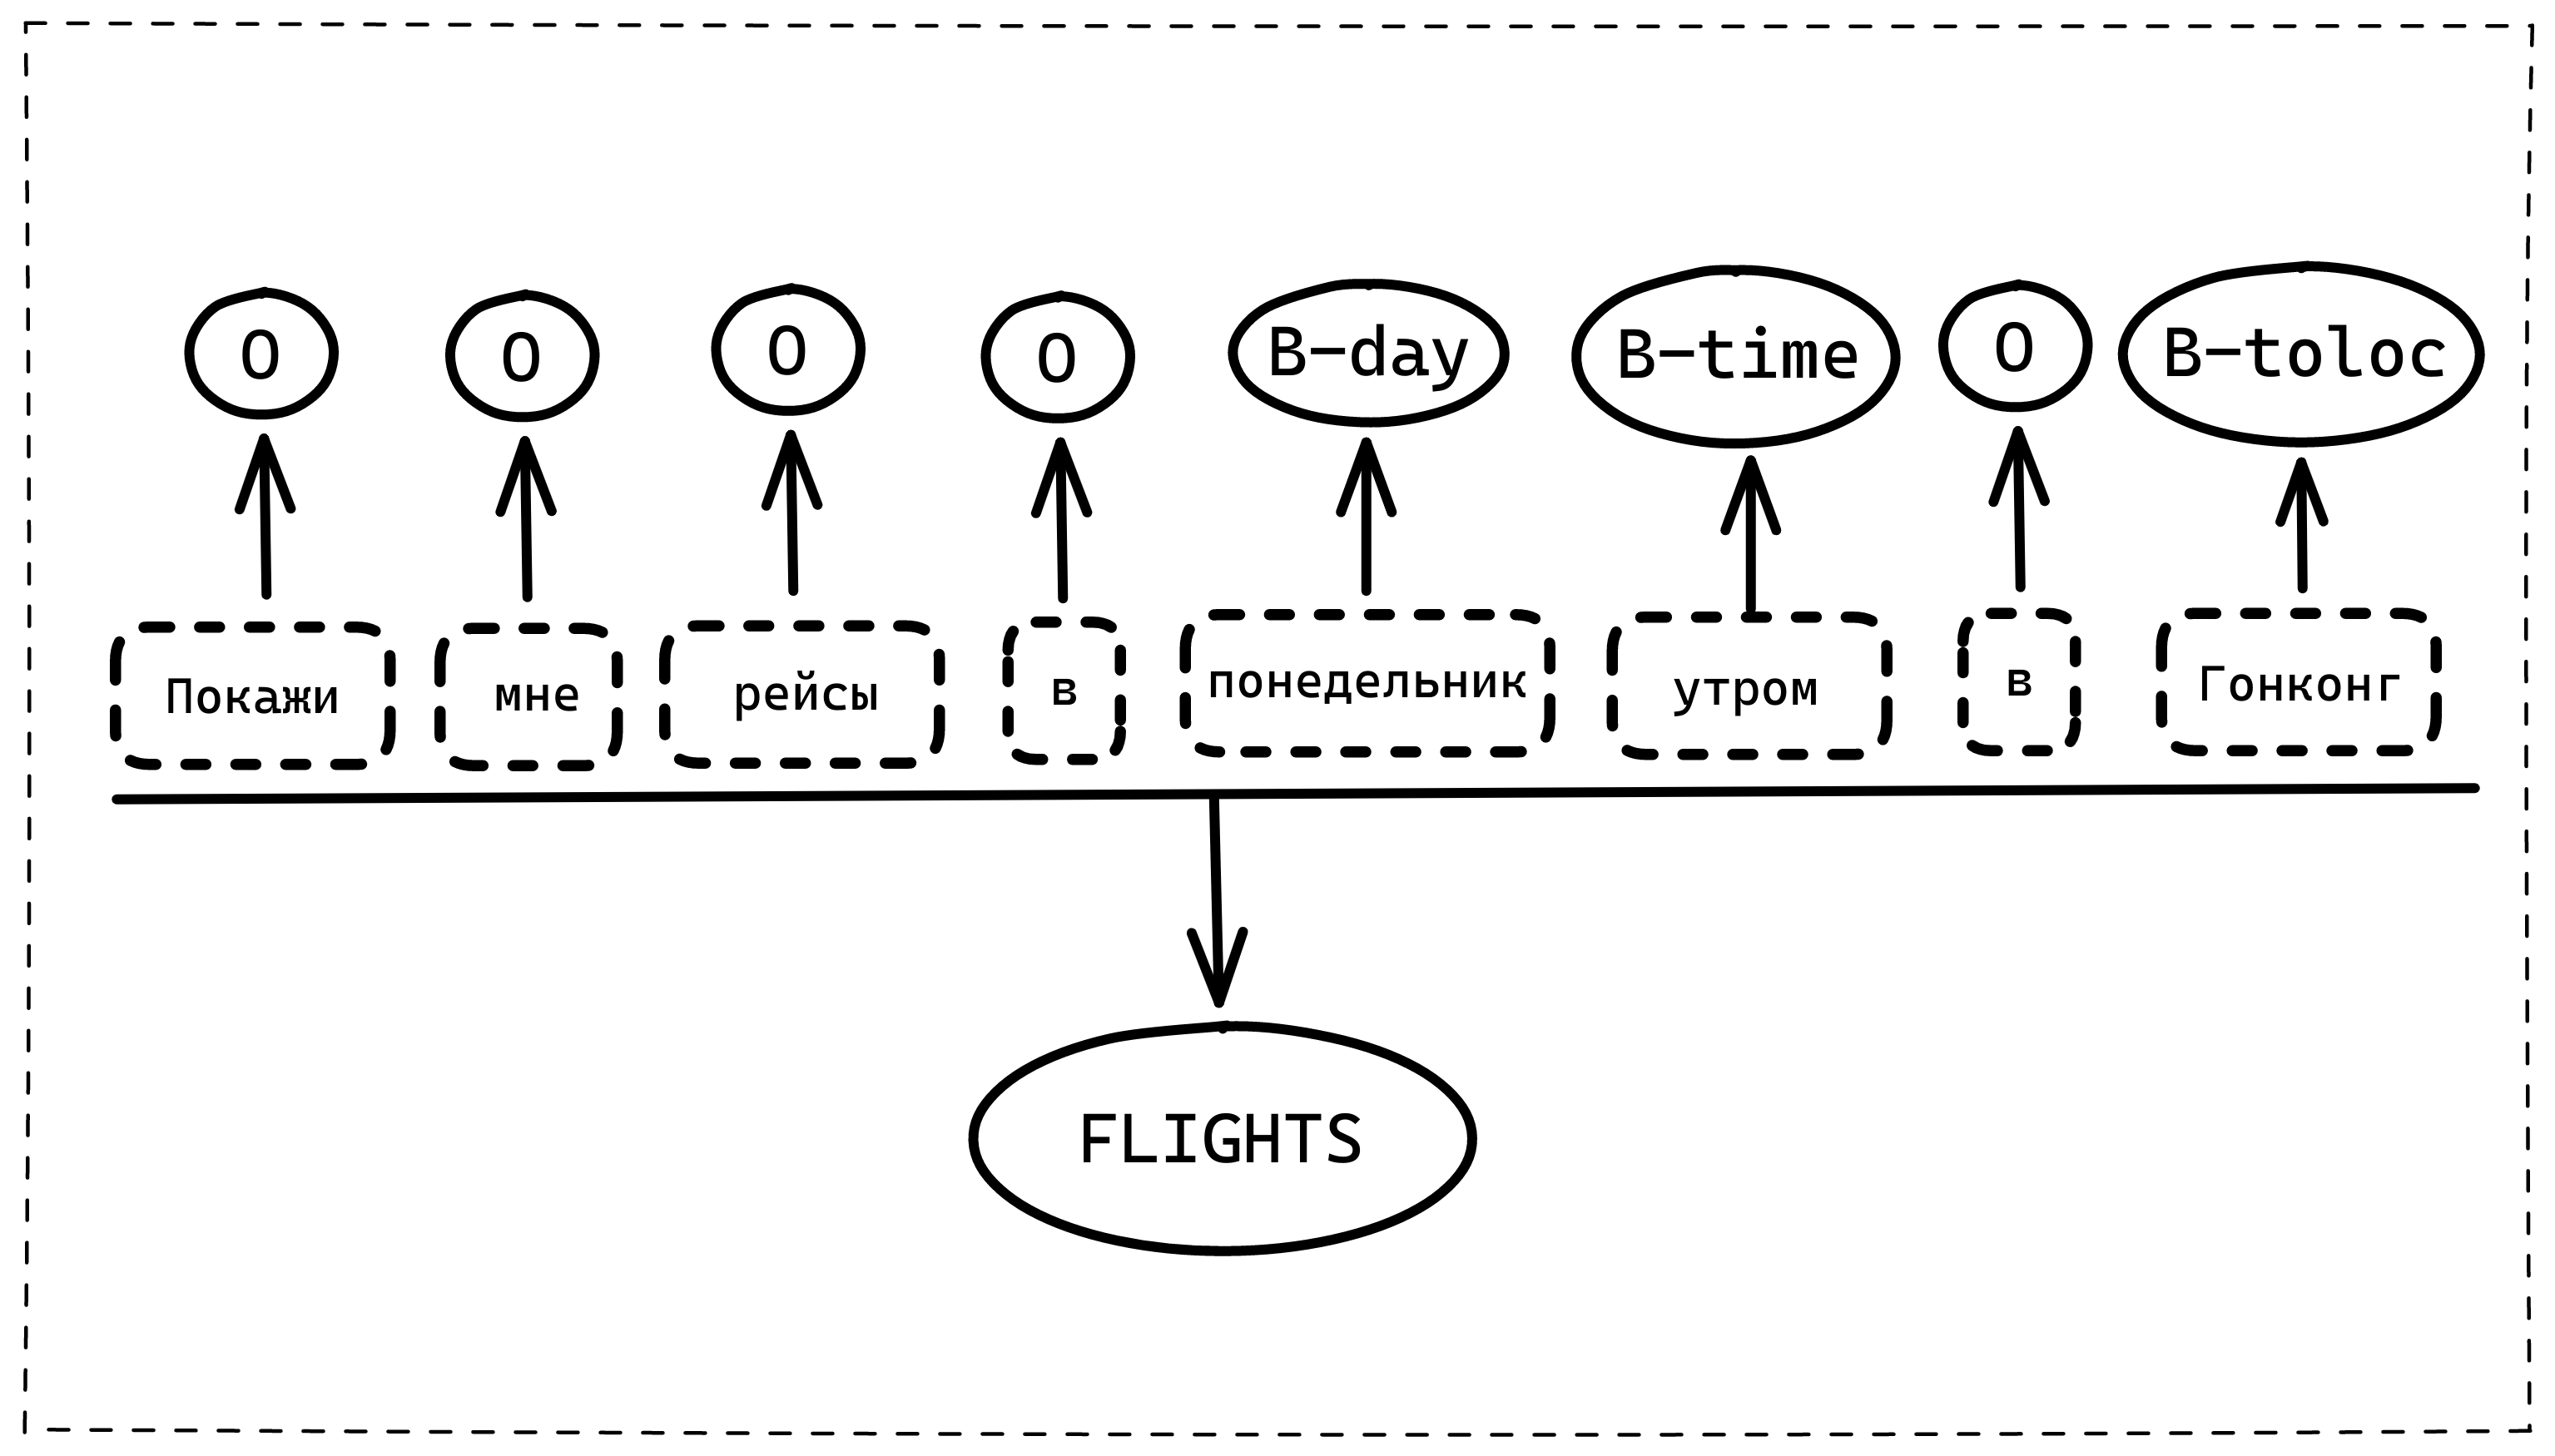
\includegraphics[width=\linewidth]{slides/4}\label{fig:figure4}
			\end{figure}
		\end{onlyenv}

		\note{В своей работе мы решаем задачу классификации интентов и заполнения слотов для диалоговых помощников. Интент — это желаемый результат запроса пользователя. Слоты — это слова или наборы слов, которые содержат релевантную интенту информацию. Таким образом, задача заключается в классификации каждого слова из предложения и всего предложения целиком. Из-за тесной корреляции между задачами заполнения слотов и классификации интентов, мы использовали в своей работе одну модель для одновременного решения обеих задач.}
	\end{frame}

	\begin{frame}{Набор данных}
		\begin{table}[H]
			\resizebox{\textwidth}{!}{
				\begin{tabular}{|>{\bfseries}c|ccccccc|}
					\hline
					Intent & \multicolumn{7}{c|}{ atis\_flight } \\ \hline
					Utterance en   & show  & me  & flights & from & montreal             & to   & orlando            \\ \hline
					Slot labels en & O     & O   & O       & O    & B-fromloc.city\_name & O    & B-toloc.city\_name \\ \hline
					Utterance de   & Zeige & mir & Flüge   & von  & Montreal             & nach & Orlando            \\ \hline
					Slot labels de & O     & O   & O       & O    & B-fromloc.city\_name & O    & B-toloc.city\_name \\ \hline
				\end{tabular}
			}\caption*{Пример объекта из набора данных MultiAtis++\cite{Xu2020EndtoEndSA}}\label{tab:table}
		\end{table}

		\note{В качестве набора данных мы выбрали корпус MultiAtis++. В этом наборе данных представлены семь языков из трех языковых семей — английский, немецкий, французский, испанский, португальский, японский и китайский. Набор данных является параллельным корпусом — в 2020 году он был переведён с английского языка на остальные шесть. В обучающей выборке содержится немногим меньше пяти тысяч предложений для каждого языка, в тестовой чуть менее тысячи предложений для каждого языка. Каждый объект состоит из предложения, меток слов в beginning, inside и outside формате и интента, как Вы можете видеть на слайде.}
	\end{frame}

	\begin{frame}{Исследуемые модели}
		\begin{onlyenv}<1>
			\begin{figure}
				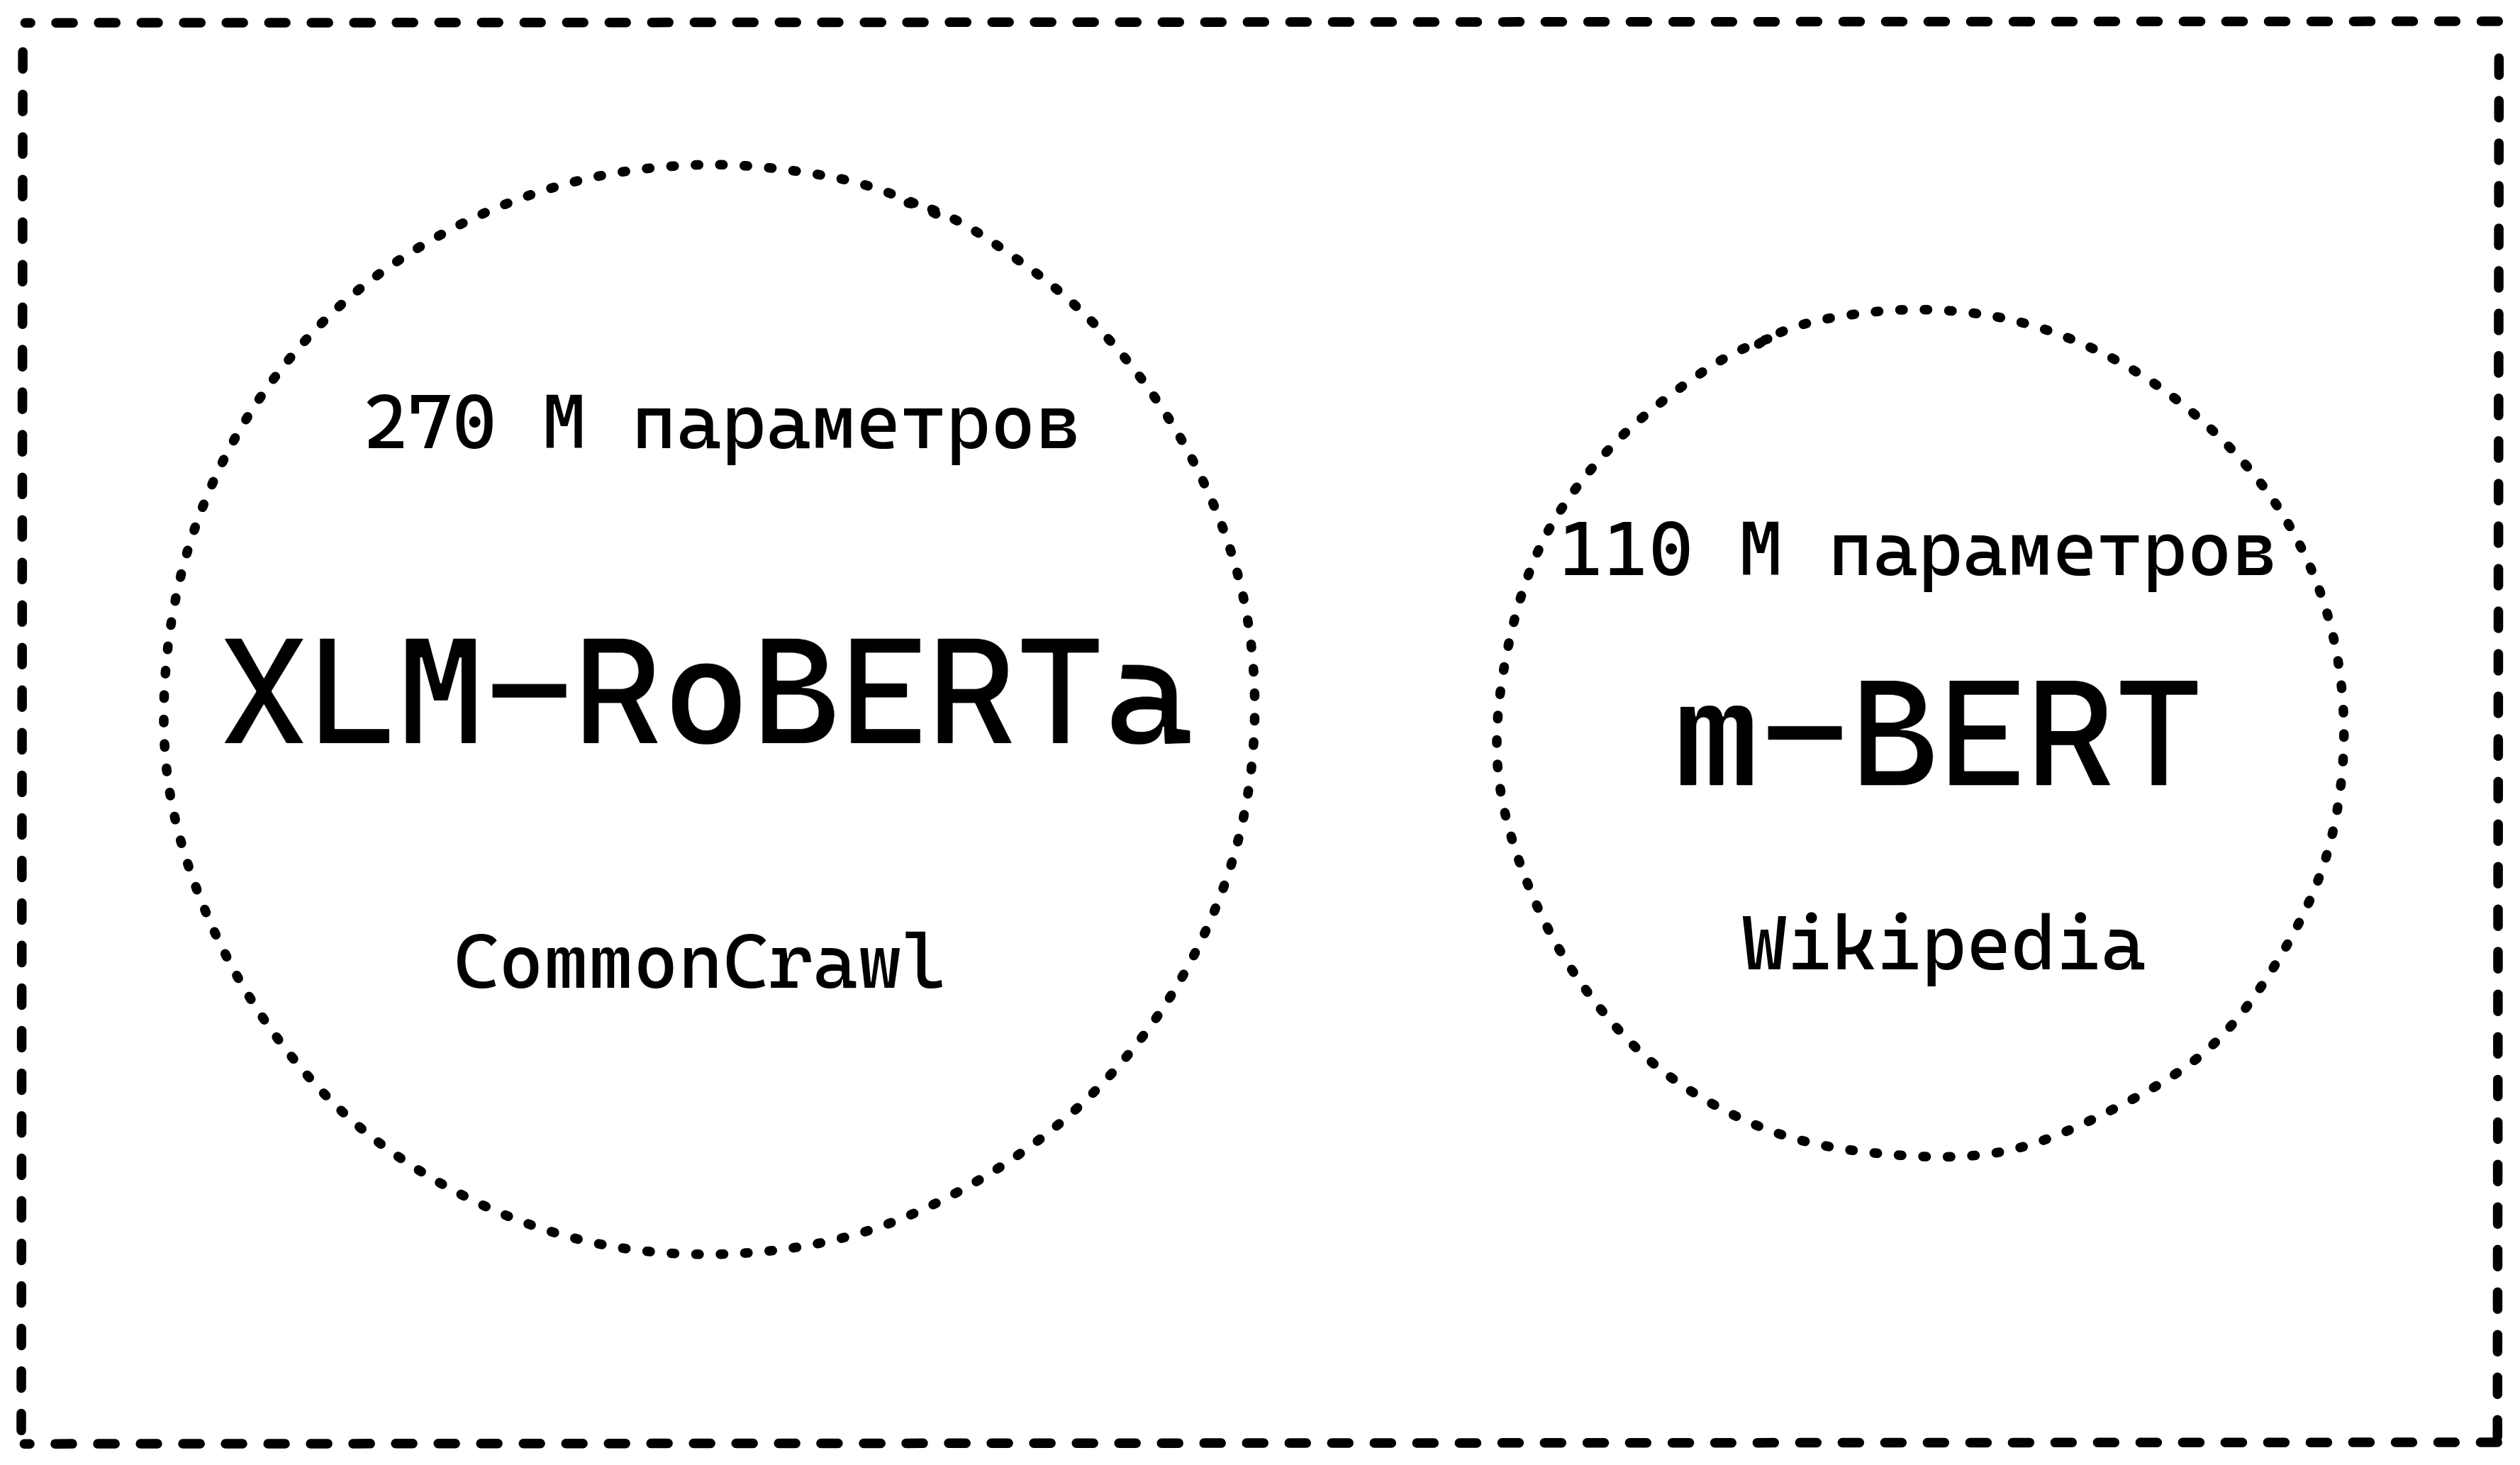
\includegraphics[width=\linewidth]{slides/5}\label{fig:figure5}
			\end{figure}
		\end{onlyenv}

		\begin{onlyenv}<2>
			\begin{figure}
				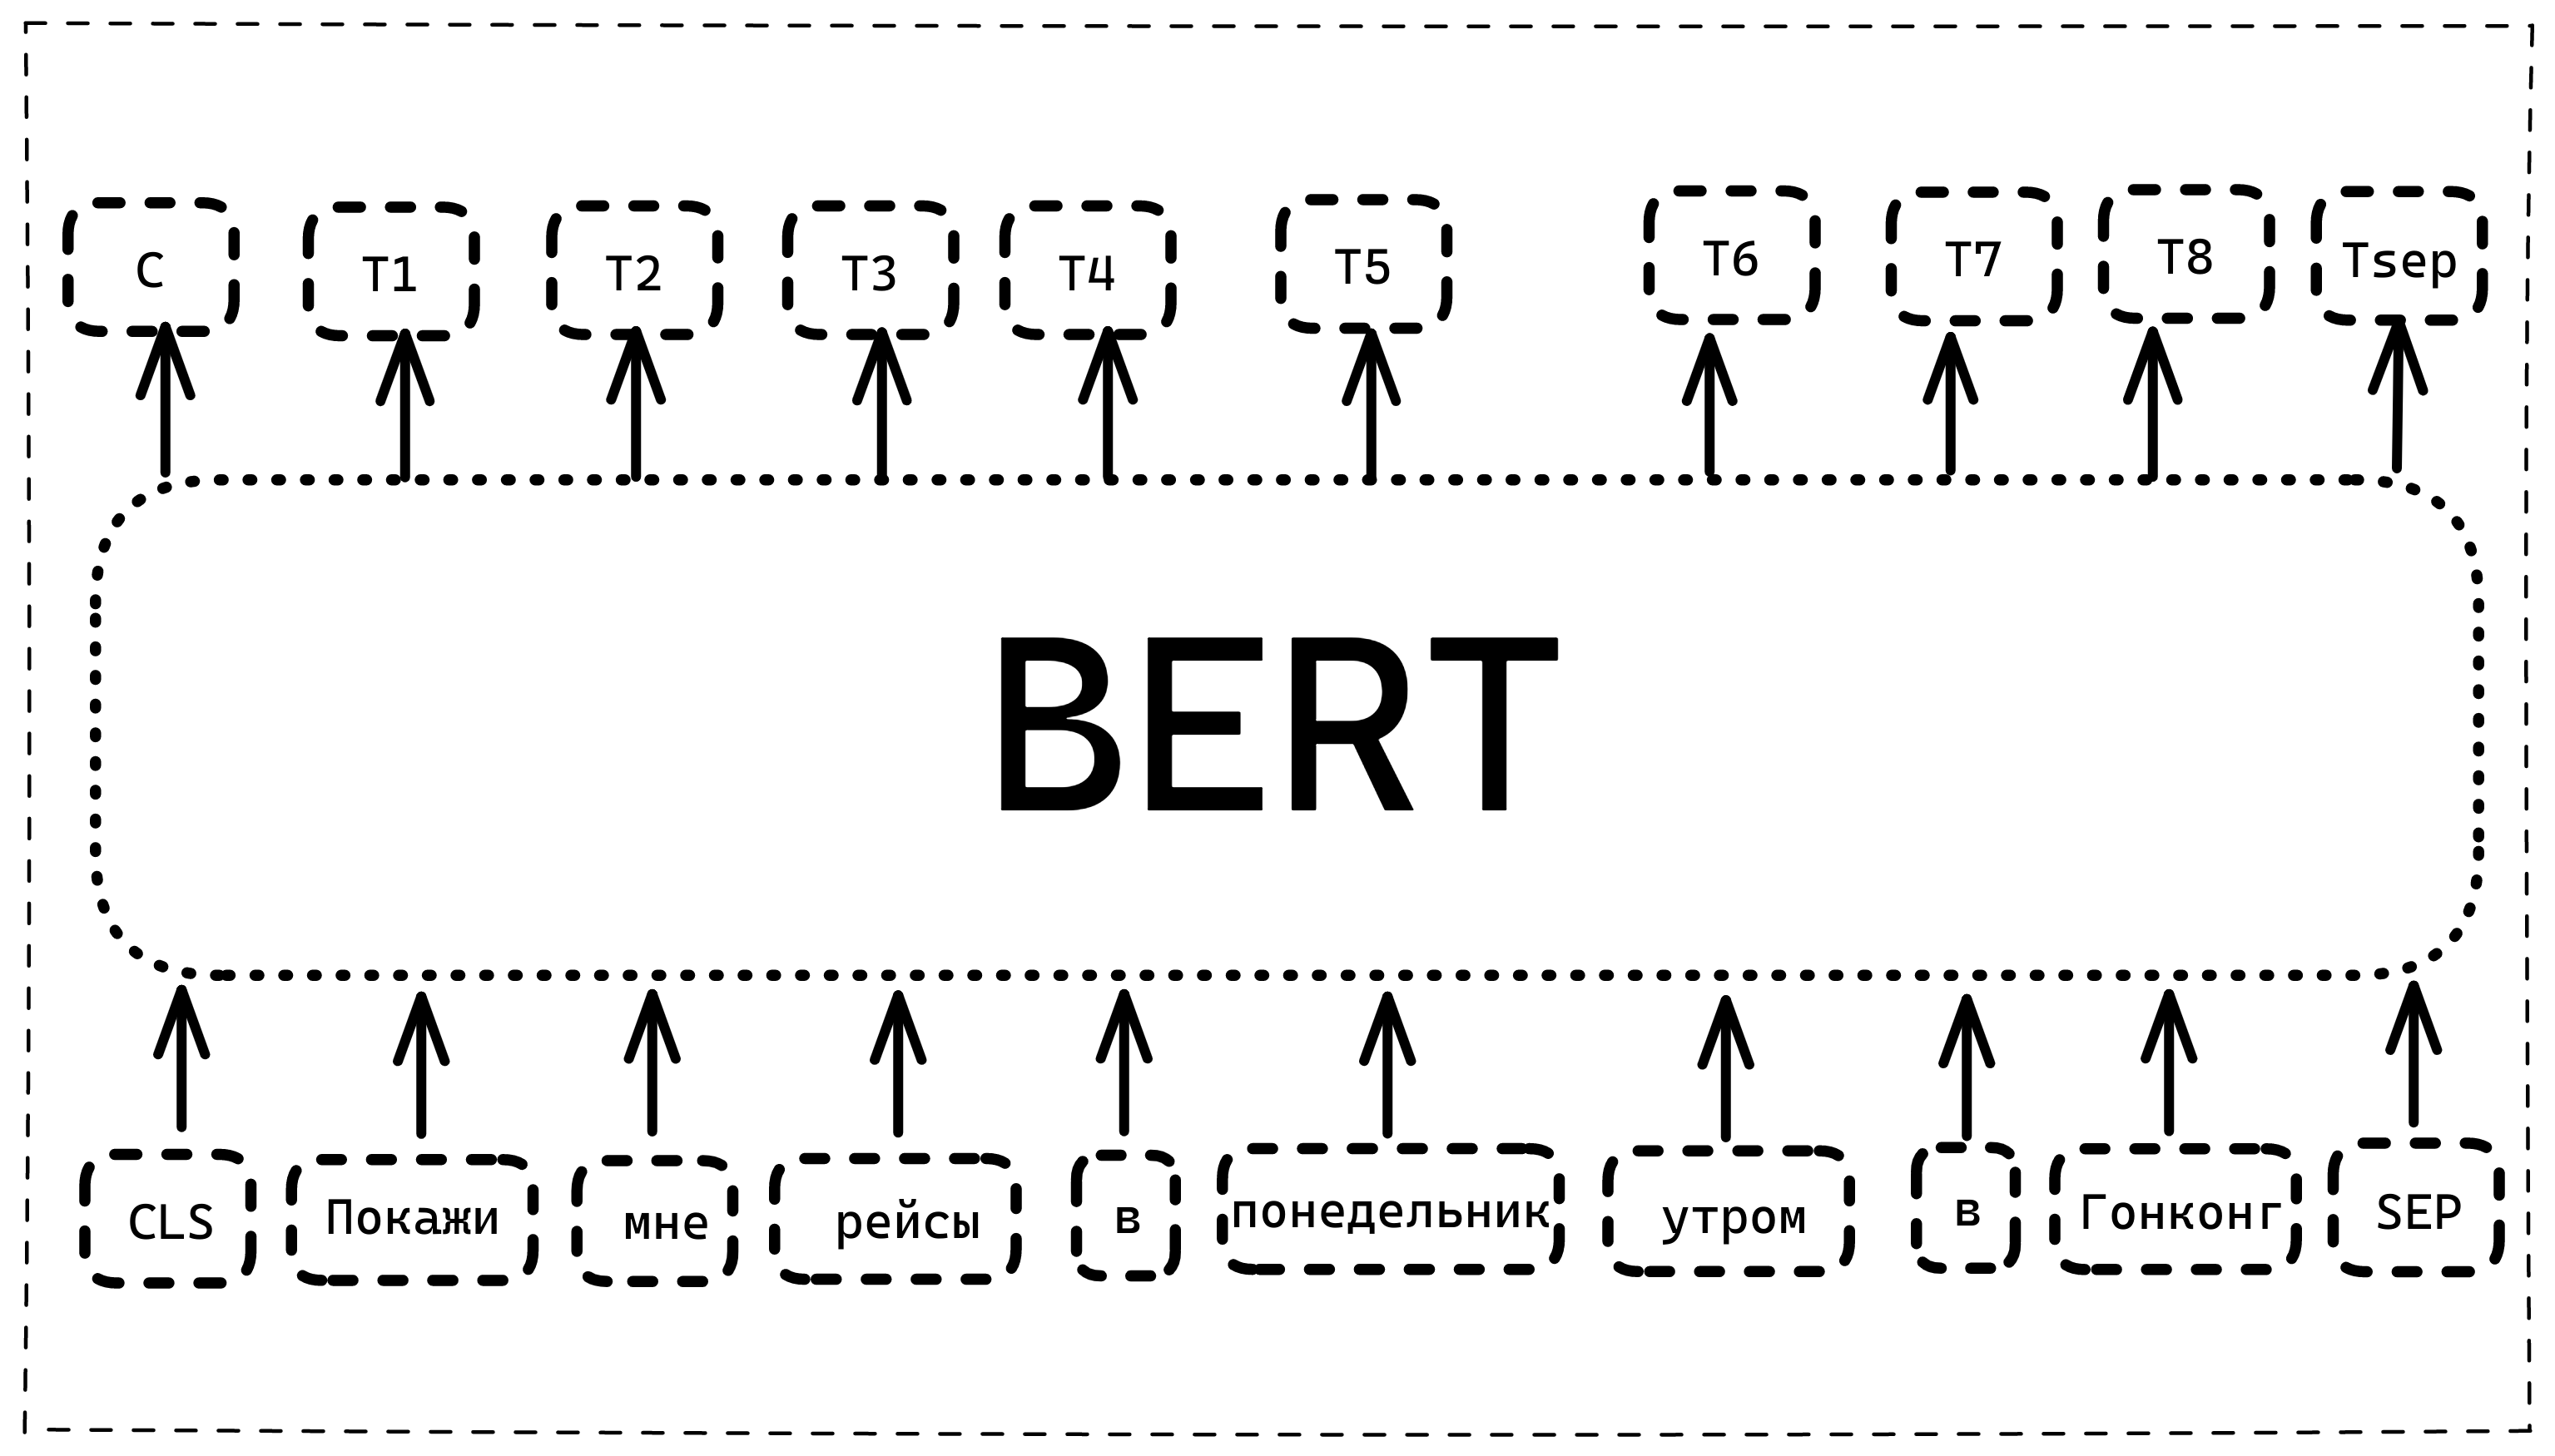
\includegraphics[width=\linewidth]{slides/13}\label{fig:figure30}
			\end{figure}
		\end{onlyenv}~\cite{Conneau2020UnsupervisedCR,devlin-etal-2019-bert}

		\note{В своей работе мы исследовали влияние смешения кодов на две предобученные мультиязычные языковые модели - m-BERT и XLM-RoBERTa. Это две мощные современные модели, обученные на более чем ста языках. Обе эти модели имеют одинаковую архитектуру, отличия между ними заключаются в методе предобучения, токенизации входных данных и размере. В m-bert более 110 миллионов параметров, в то время как в xlm-r более 270 миллионов. В дополнение к этому, xlm-r предобучалась на наборе данных CommonCrawl, а m-bert на Wikipedia, который на несколько порядков меньше.\newlineИспользуемая архитектура выглядит следующим образом - рассмотрим входную последовательность, для модели m-bert токенизируем её с помощью WordPiece, для модели xlm-r с помощью byte pair encoding. Затем мы обрамляем токенизированную последовательность специальными токенами CLS и SEP и подаем на вход модели. Затем мы подаем выход модели по токену CLS в линейный слой - голову по интентам и получаем классификацию интентов. А выход модели по всем следующим токенам кроме SEP подаем на вход линейному слою - голове по слотам и получаем классификацию по слотам для каждого слова в предложении.}
	\end{frame}

%------------------------------------------------


	\section{Адверсариальные атаки}
%------------------------------------------------

	\begin{frame}{Предлагаемые атаки}
		\begin{figure}
			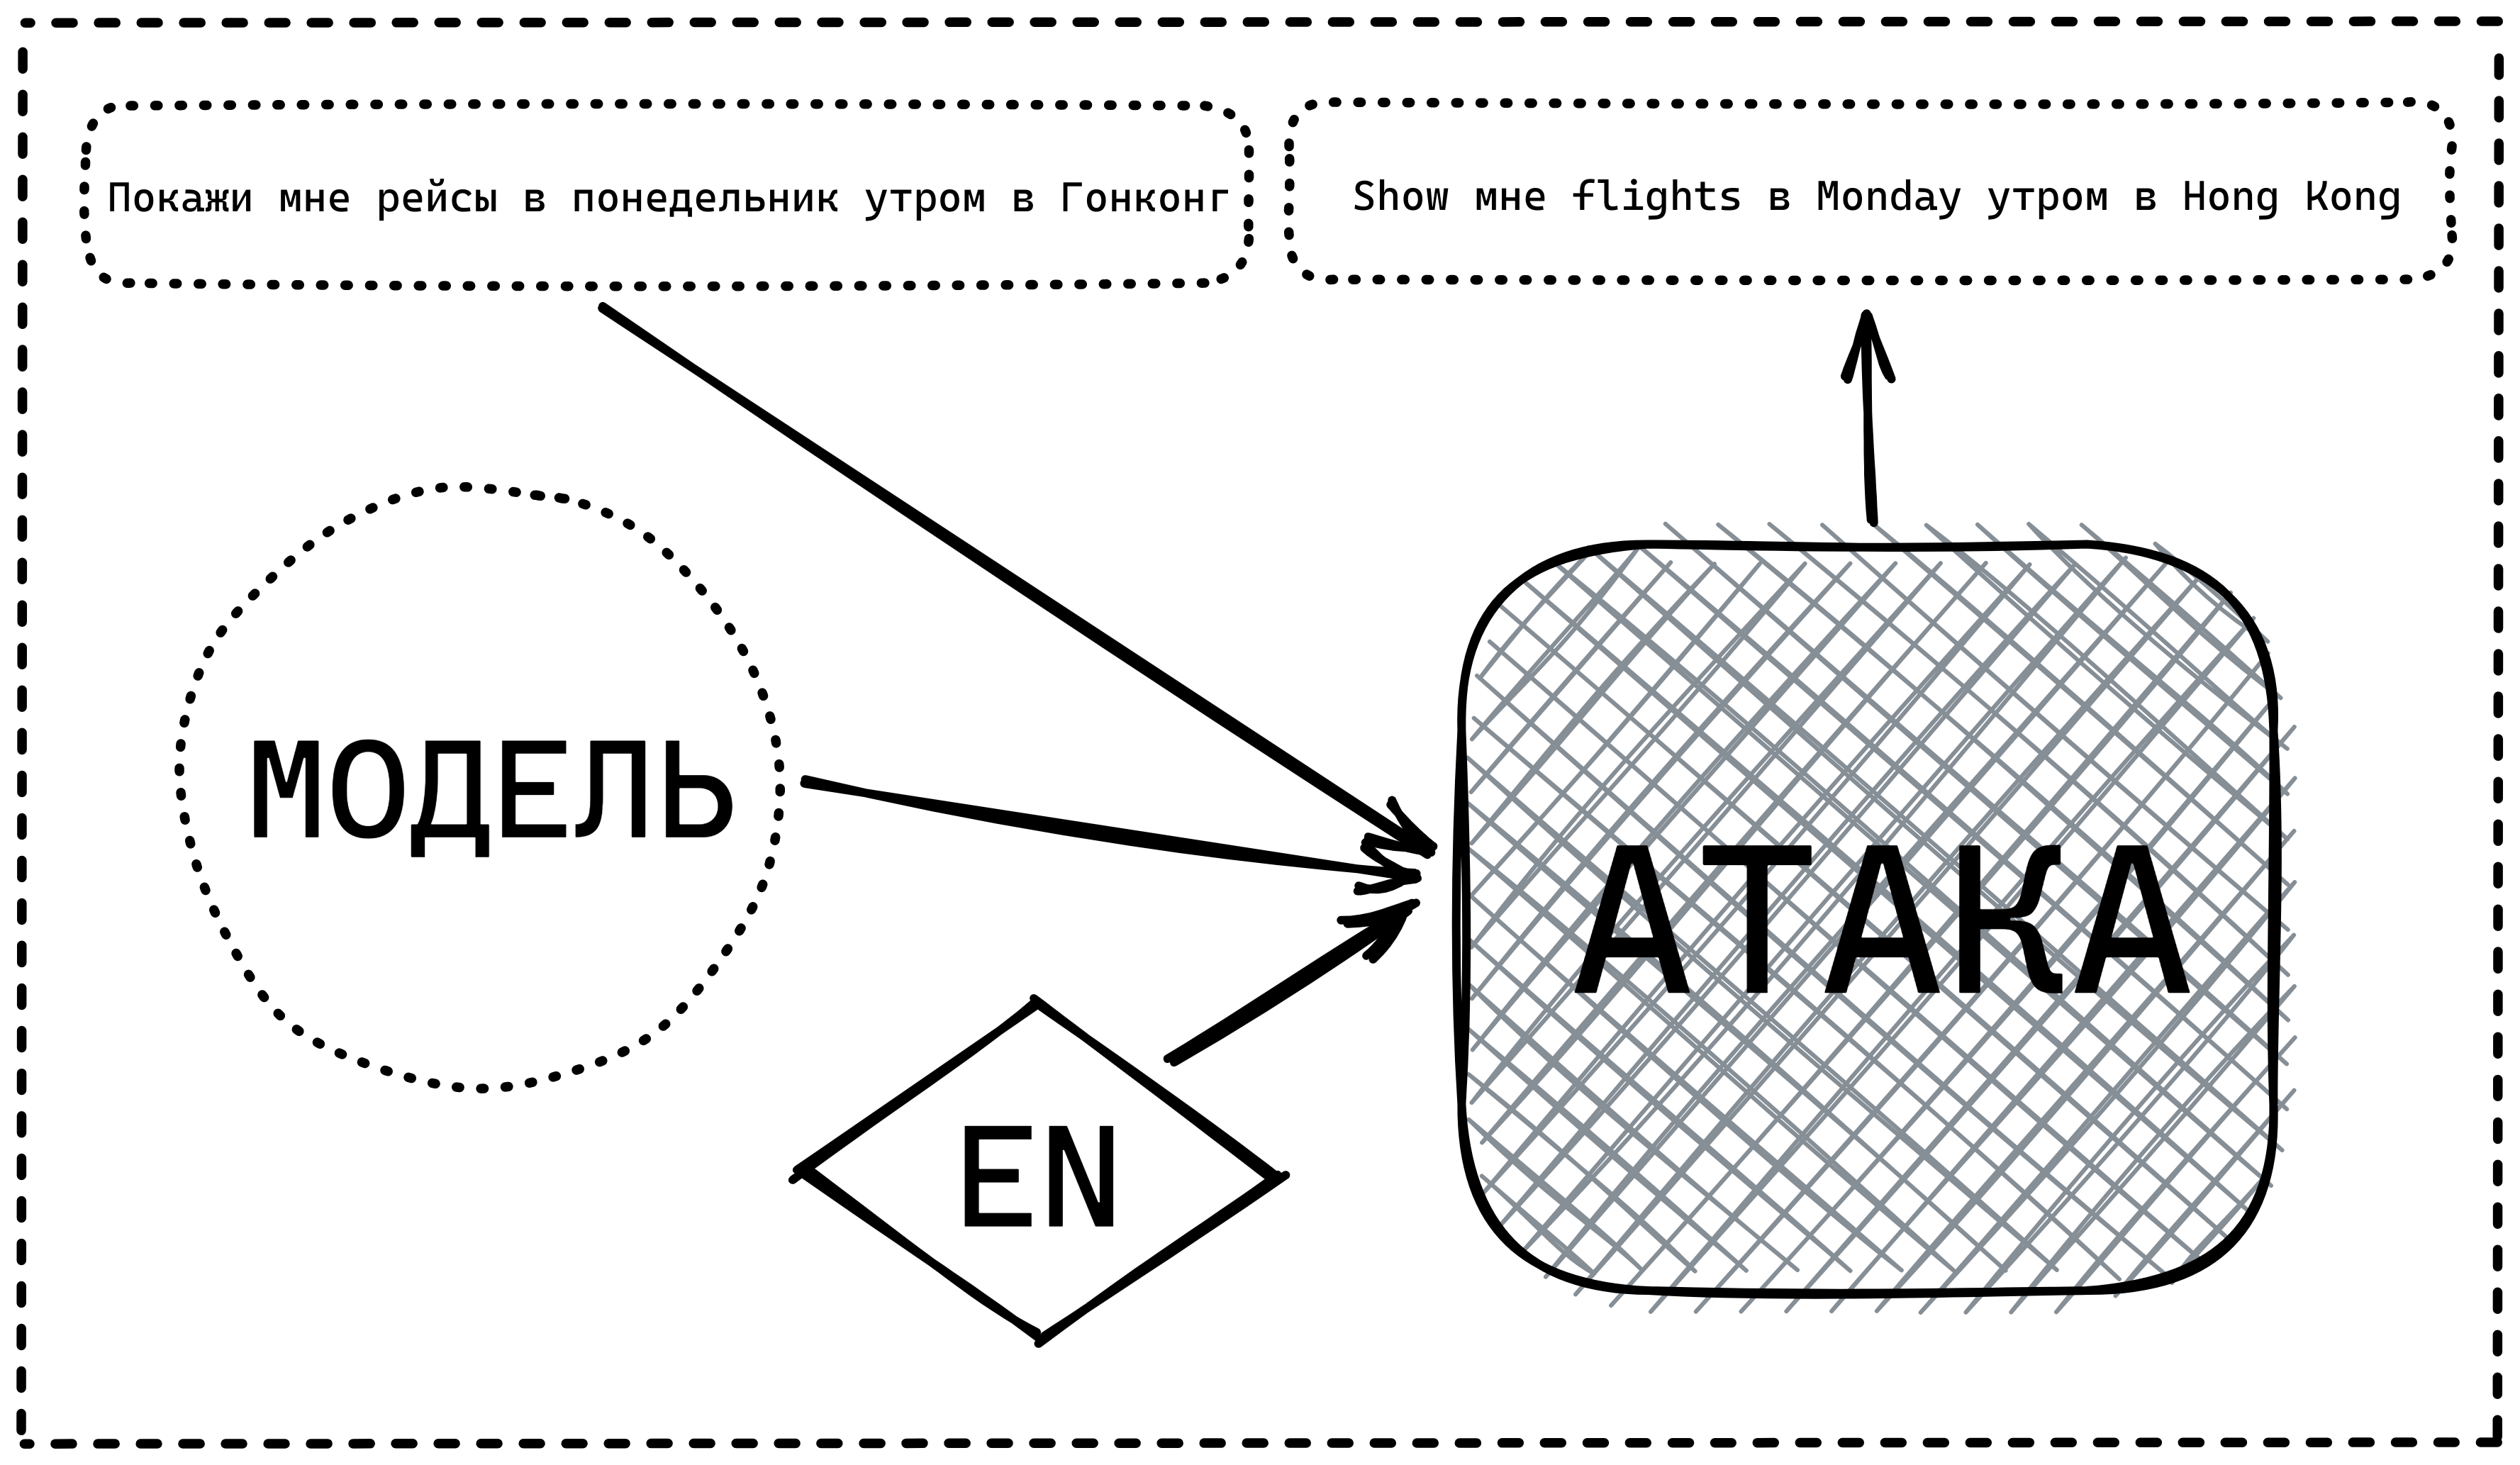
\includegraphics[width=\linewidth]{slides/6}\label{fig:figure6}
		\end{figure}

		\note{В своей работе мы предлагаем два варианта атак, оба варианта по схеме серого ящика — во время выполнения атаки мы имеем доступ к ошибке модели на входных данных. Мы стремимся создать атаку такого рода, чтобы результирующая пертурбация предложения была похожа на реальные данные со смешением кодов и параллельно максимизируем ошибку модели. Мы фокусируемся в основном на лексической части смешения кодов — когда некоторые слова заменяются на их аналоги из других языков. Во время атаки мы заменяем часть токенов в предложении на их эквиваленты из атакующих языков, метод определения кандидатов на замену зависит от типа атаки. Так как большинство людей, которые могут использовать смешение кодов в своей речи, билингвы, то в основном смешение кодов происходит между парой языков. Таким образом, в своей работе мы анализировали атаки, которые состоят во встраивании одного языка в другой. Атаковать мы всегда будем английский.\newlineОбщий принцип атаки одинаковый для обоих предлагаемых вариантов — пусть мы имеем целевую модель, пару предложение-метка и атакующий язык. Тогда мы перебираем токены в предложении и стремимся подобрать для каждого замену из атакующего языка. Если удается увеличить ошибку модели, то мы изменяем предложение и идем дальше.}
	\end{frame}

	\begin{frame}{Word-level атака}
		\begin{figure}
			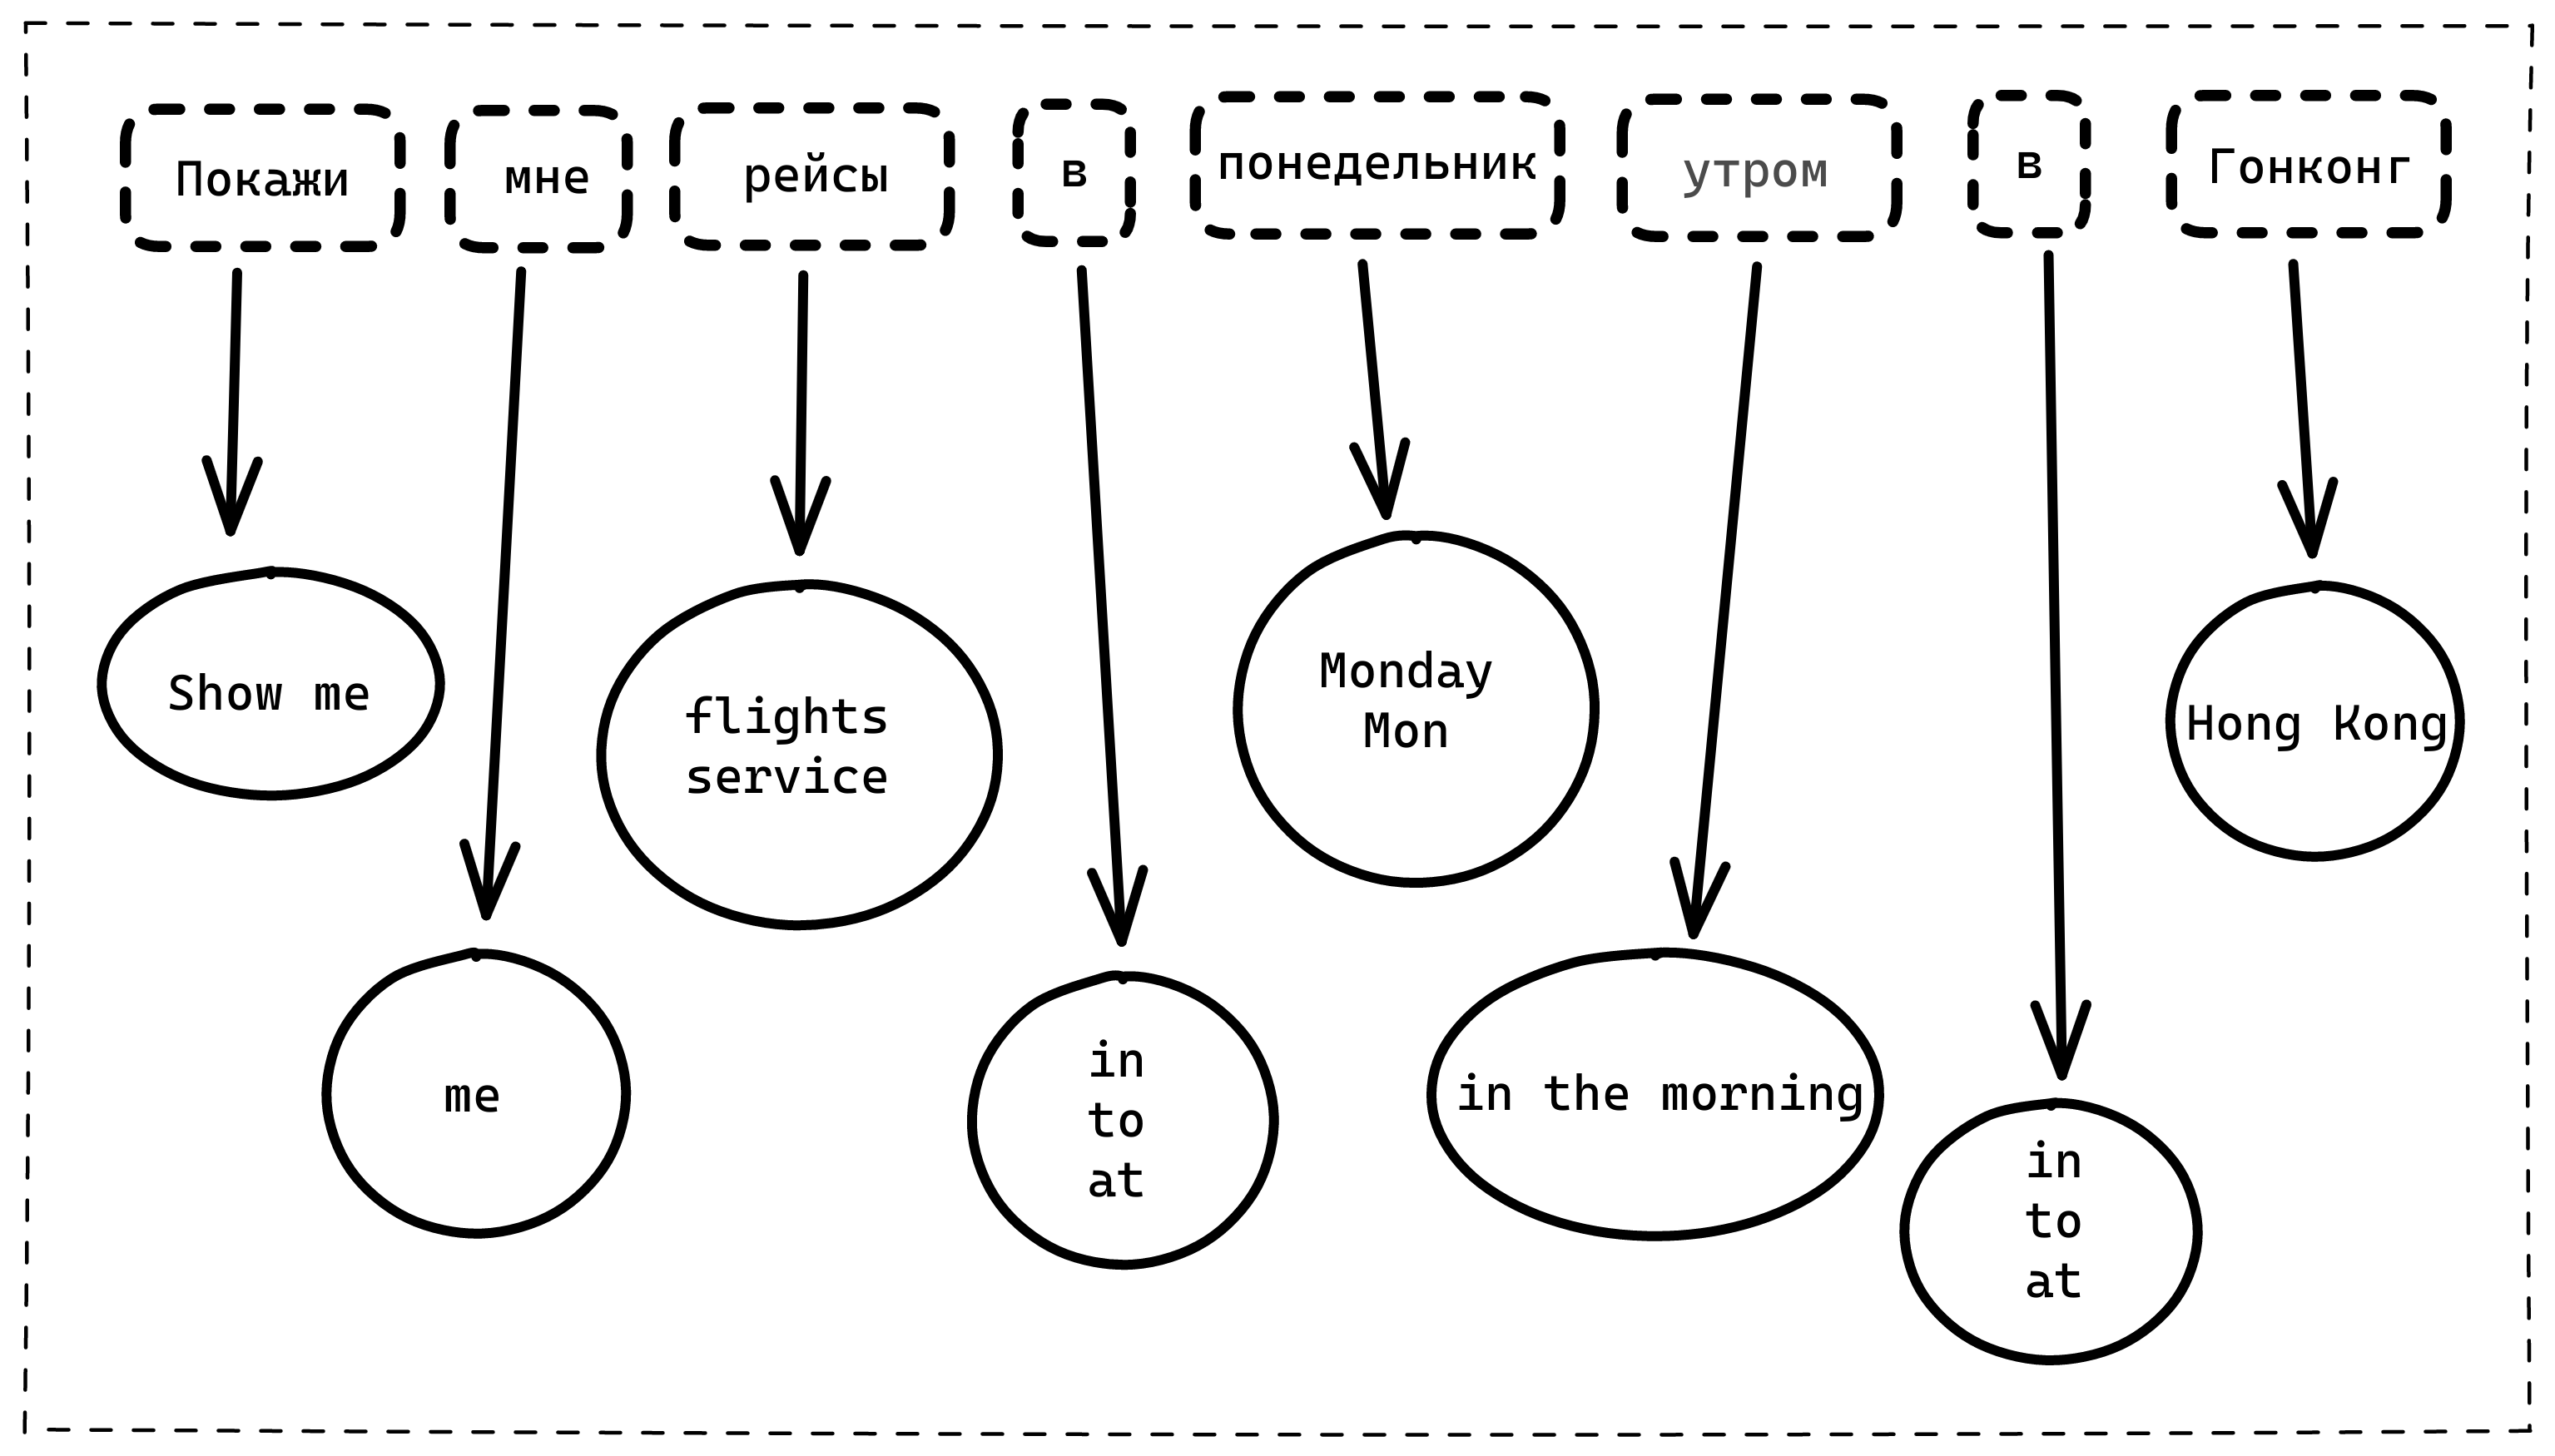
\includegraphics[width=\linewidth]{slides/7}\label{fig:figure7}
		\end{figure}

		\note{Первый предлагаемый вариант атаки называется word-level, и он заключается в генерации кандидатов на замену с помощью простого перевода отдельных слов на другие языки. Атакуя таким образом, мы строим достаточно грубую оценку снизу, так как при атаке мы не учитываем контекст предложения для перевода слова.}
	\end{frame}

	\begin{frame}{Phrase-level атака}
		\begin{figure}
			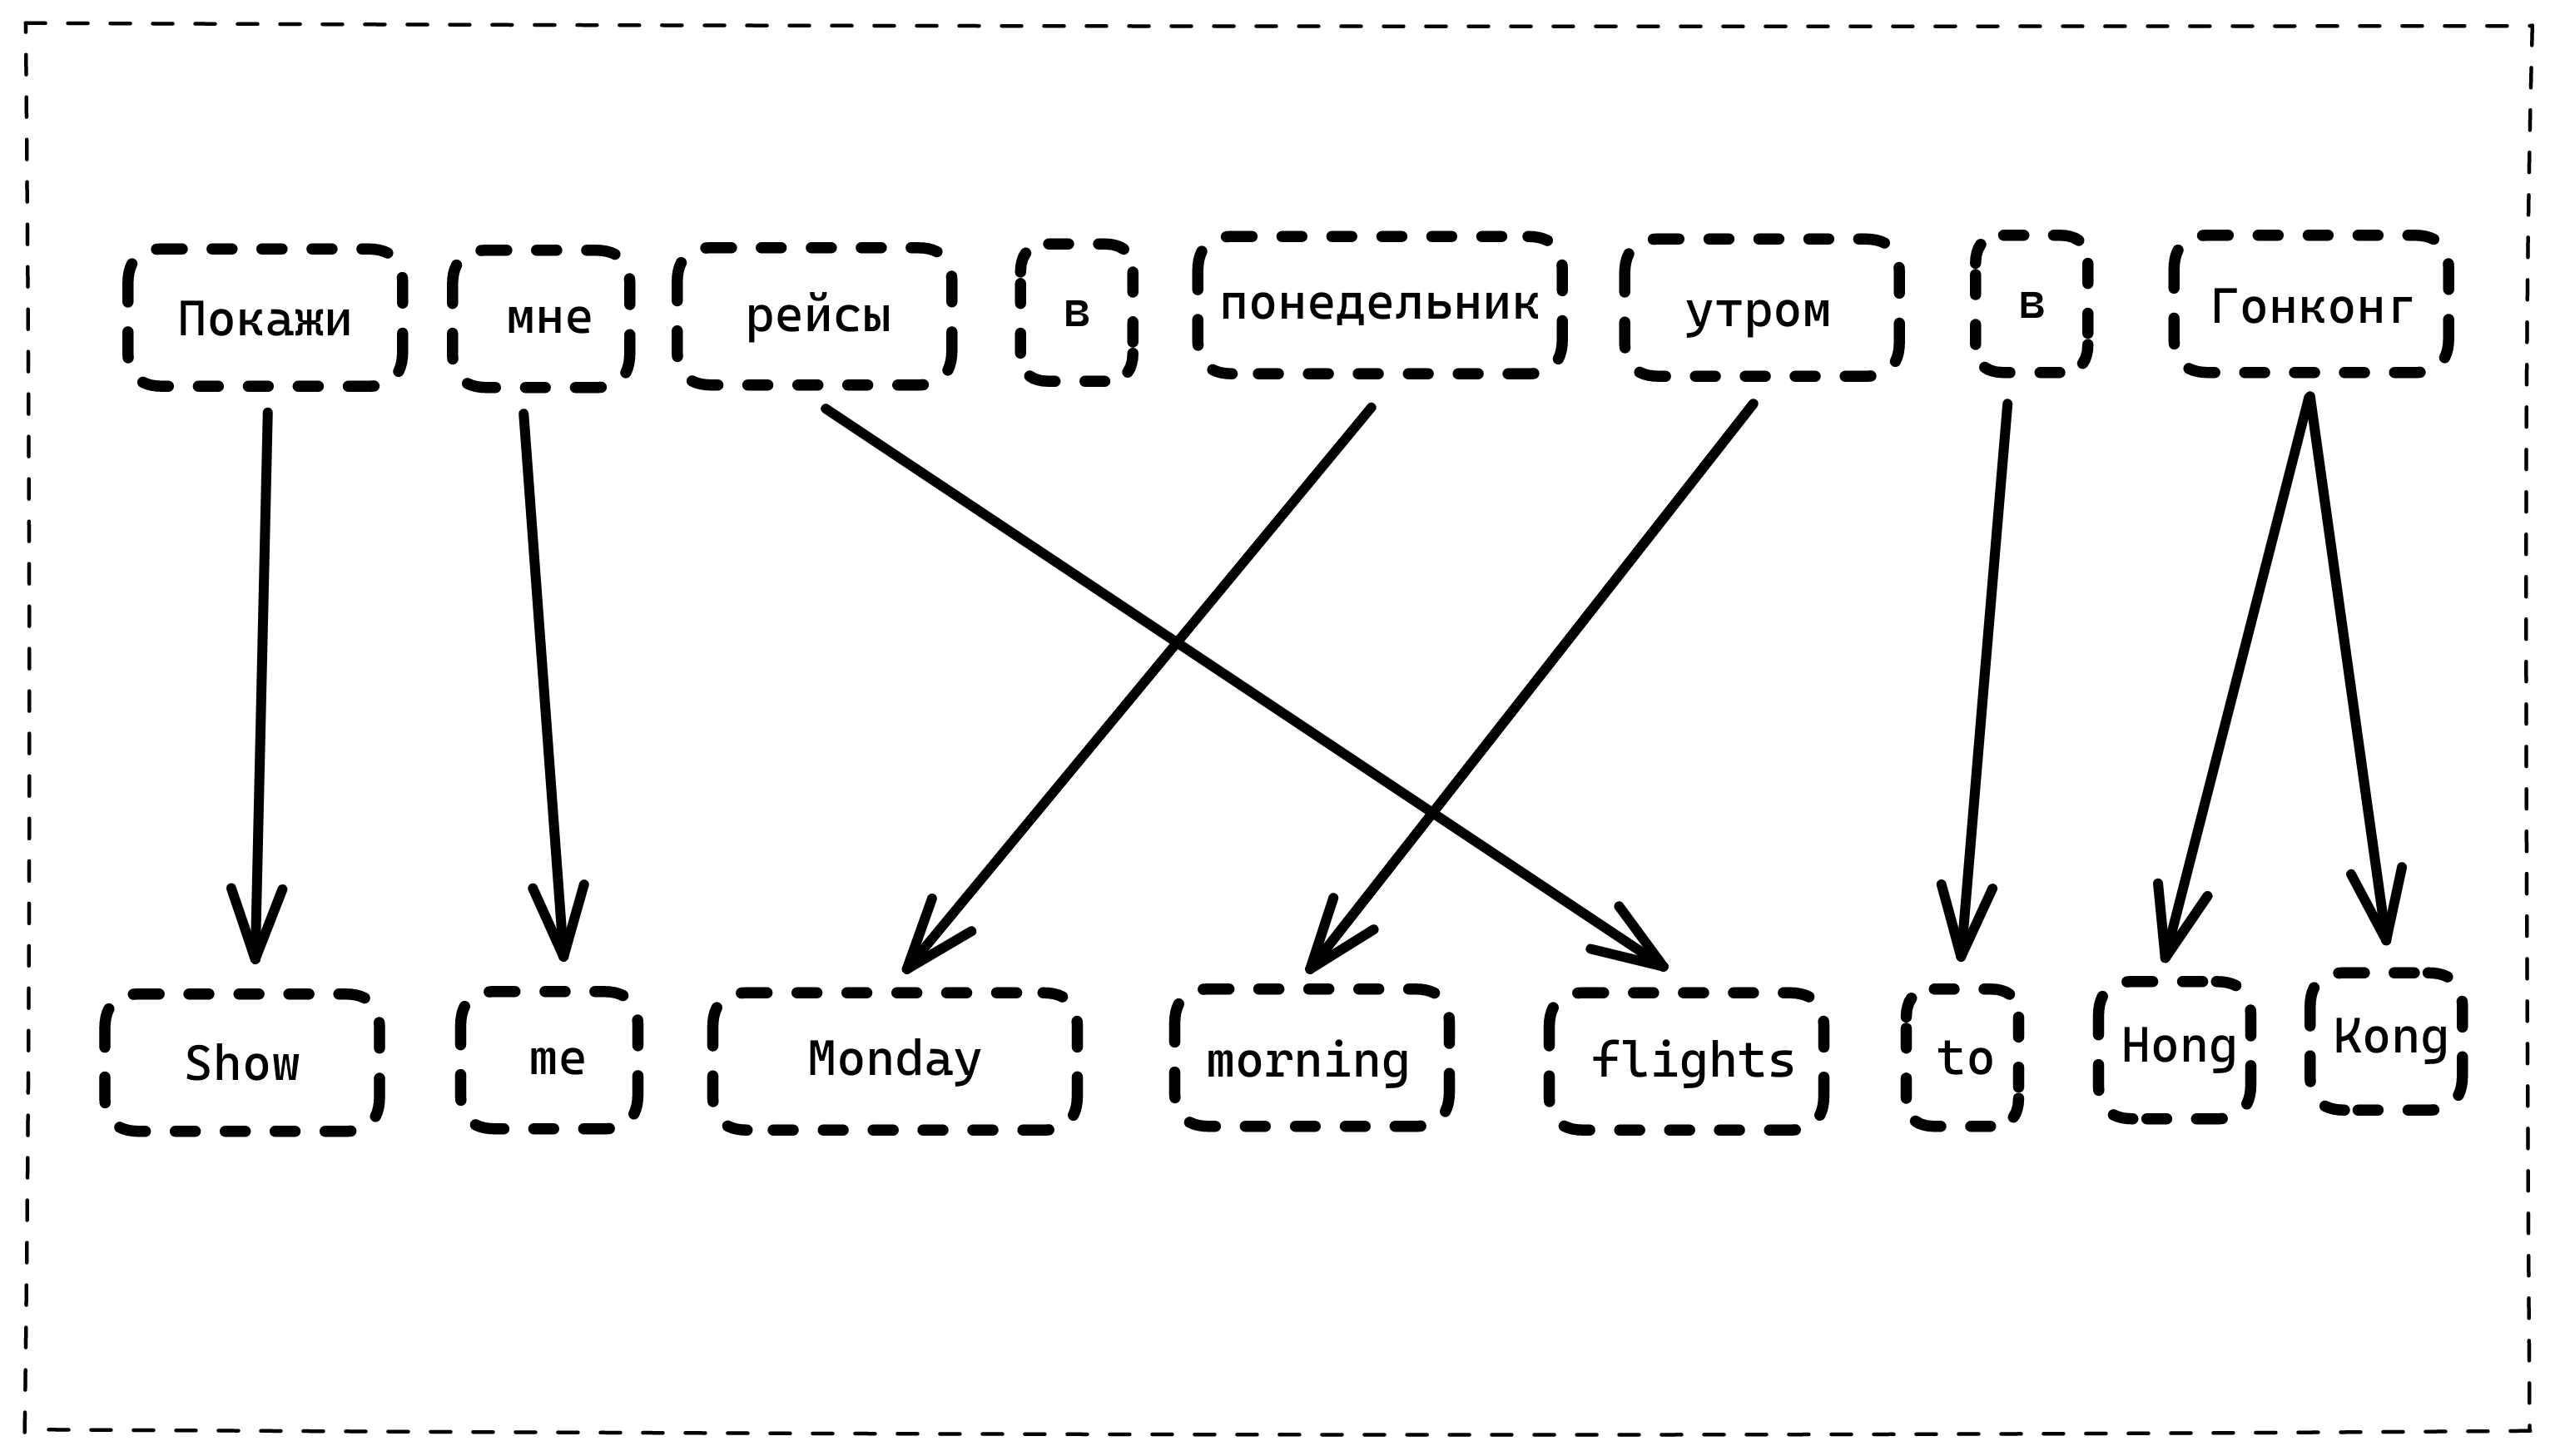
\includegraphics[width=\linewidth]{slides/8}\label{fig:figure8}
		\end{figure}

		\note{Второй предлагаемый вариант атаки называется phrase-level, и он заключается в генерации кандидатов на замену с помощью построения выравниваний между предложениями на разных языках. Кандидаты определяются с помощью выравниваний — забираем те токены, куда ведет выравнивание.}
	\end{frame}

%------------------------------------------------


	\section{Адверсариальное предобучение}

%------------------------------------------------

	\begin{frame}{Метод адверсариального предобучения}
		\begin{onlyenv}<1>
			\begin{figure}
				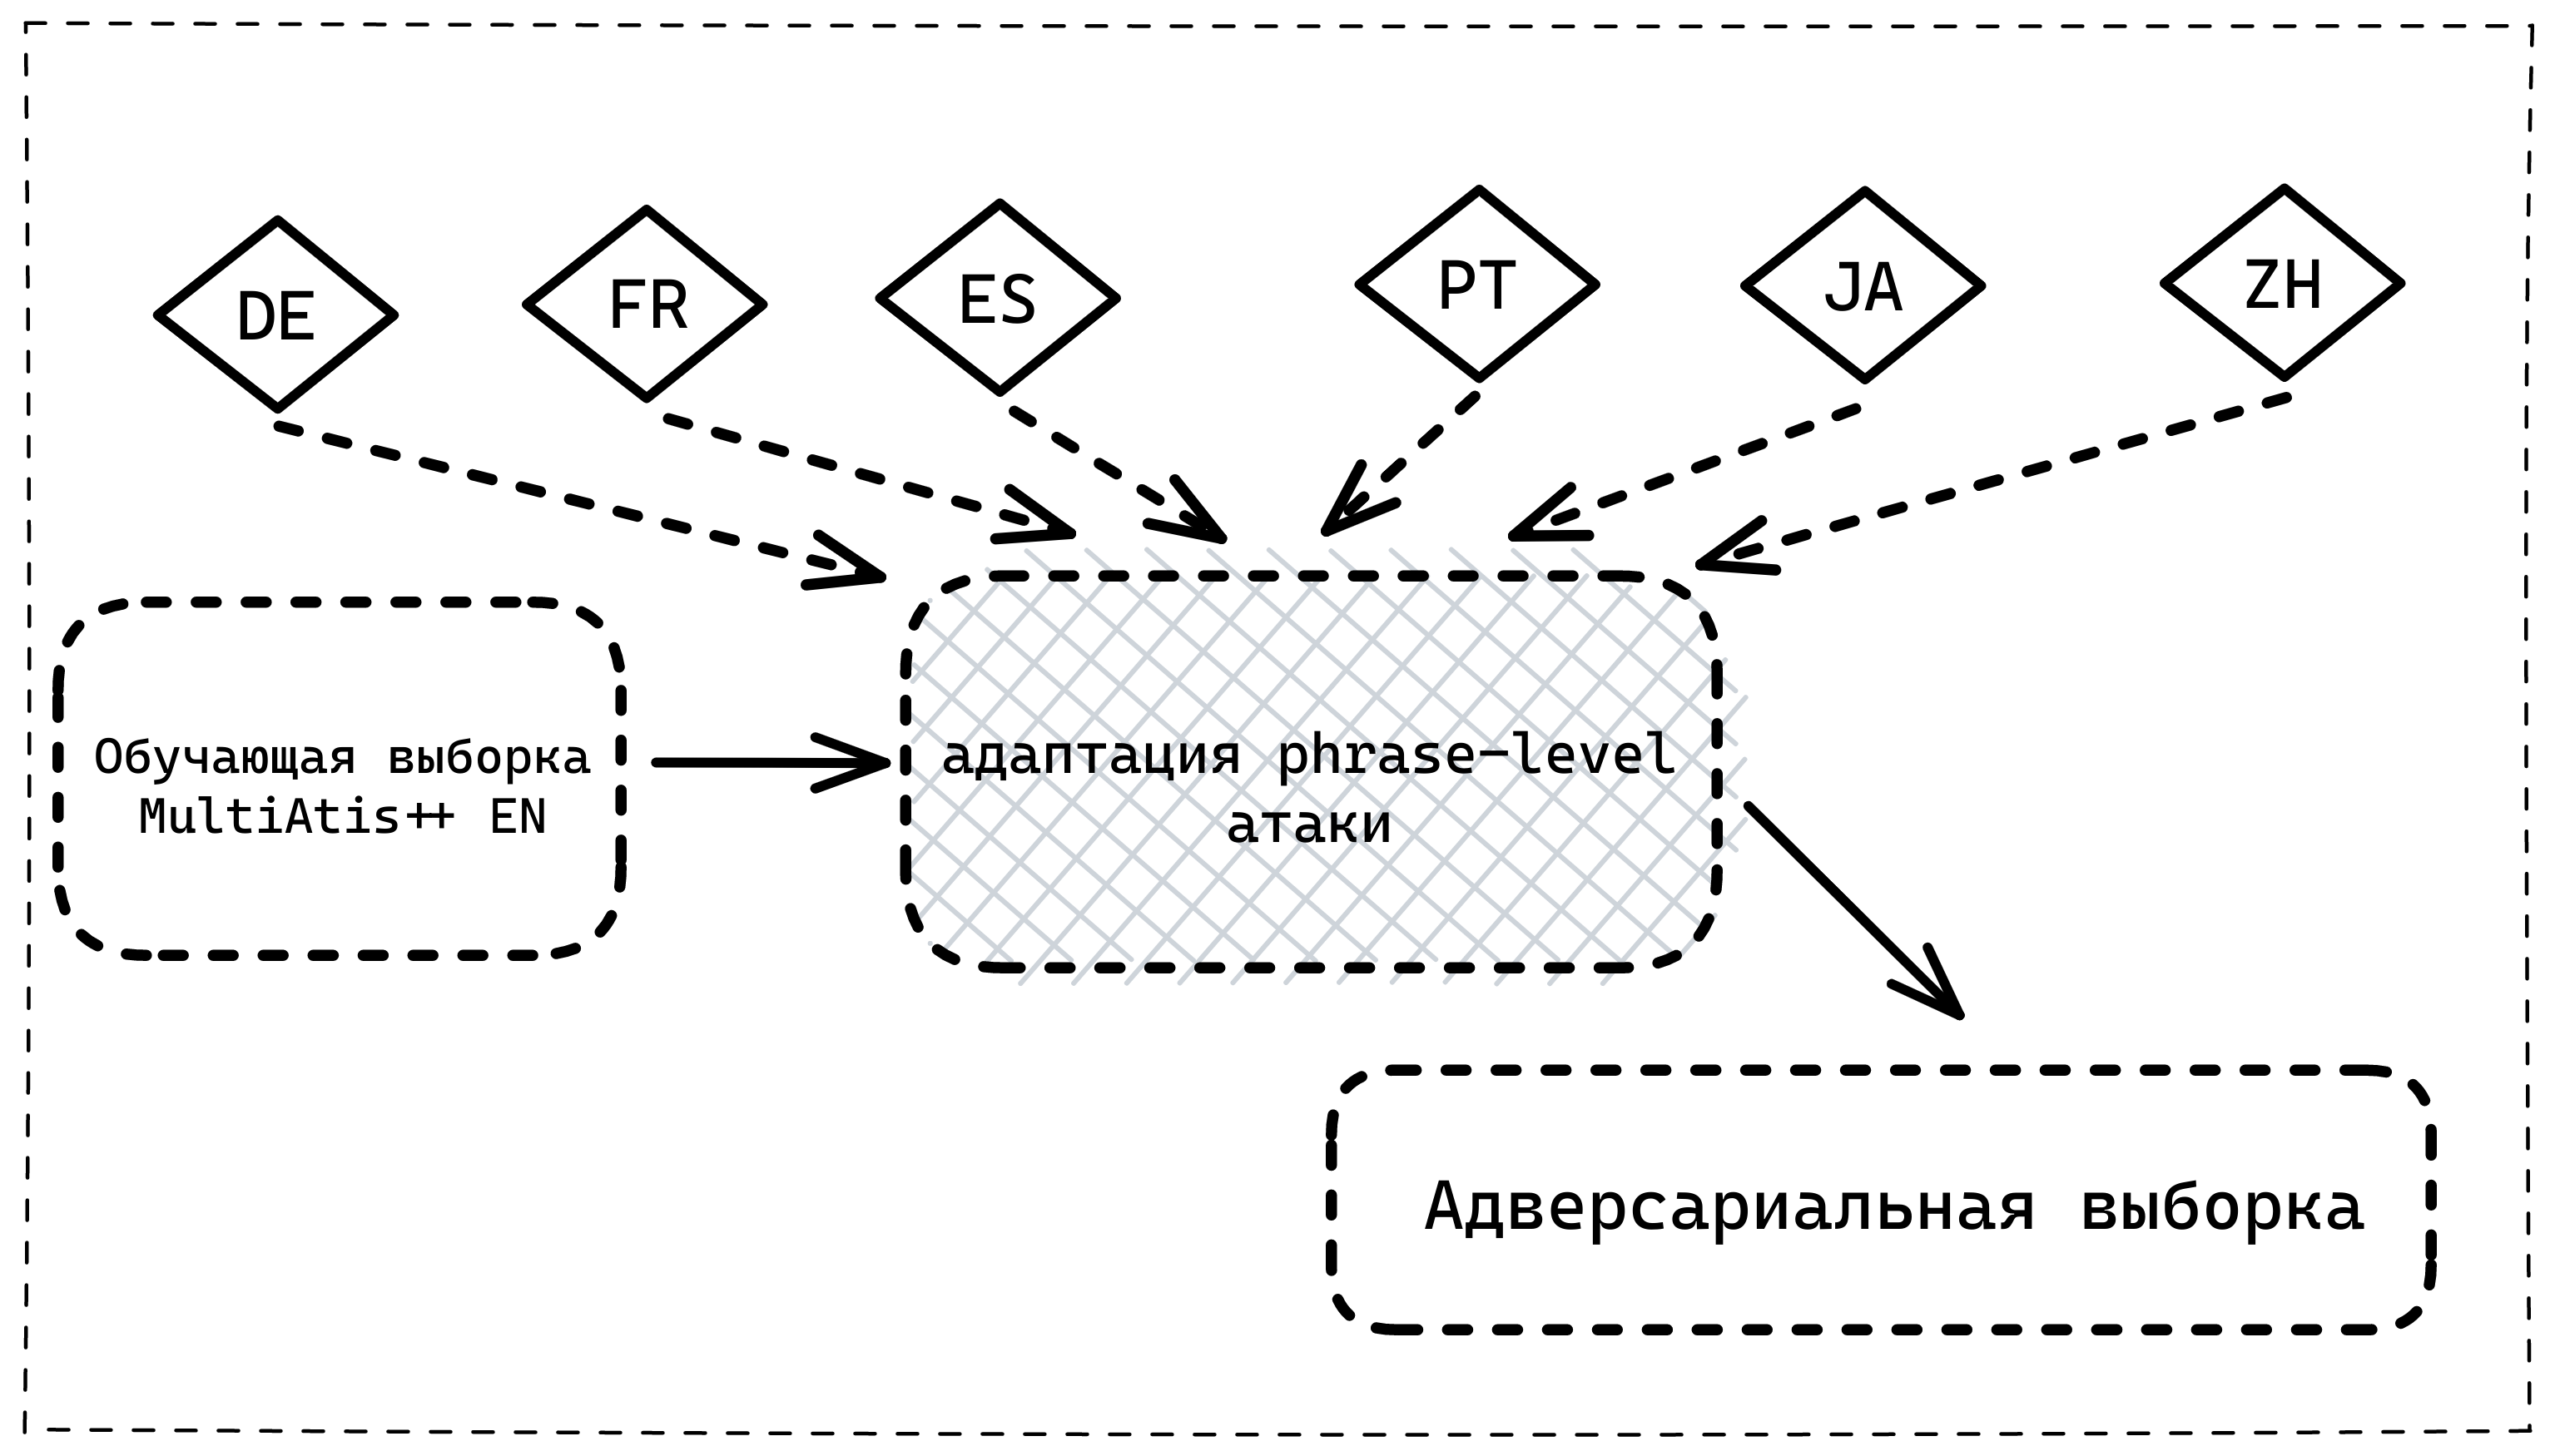
\includegraphics[width=\linewidth]{slides/9}\label{fig:figure9}
			\end{figure}
		\end{onlyenv}

		\begin{onlyenv}<2>
			\begin{figure}
				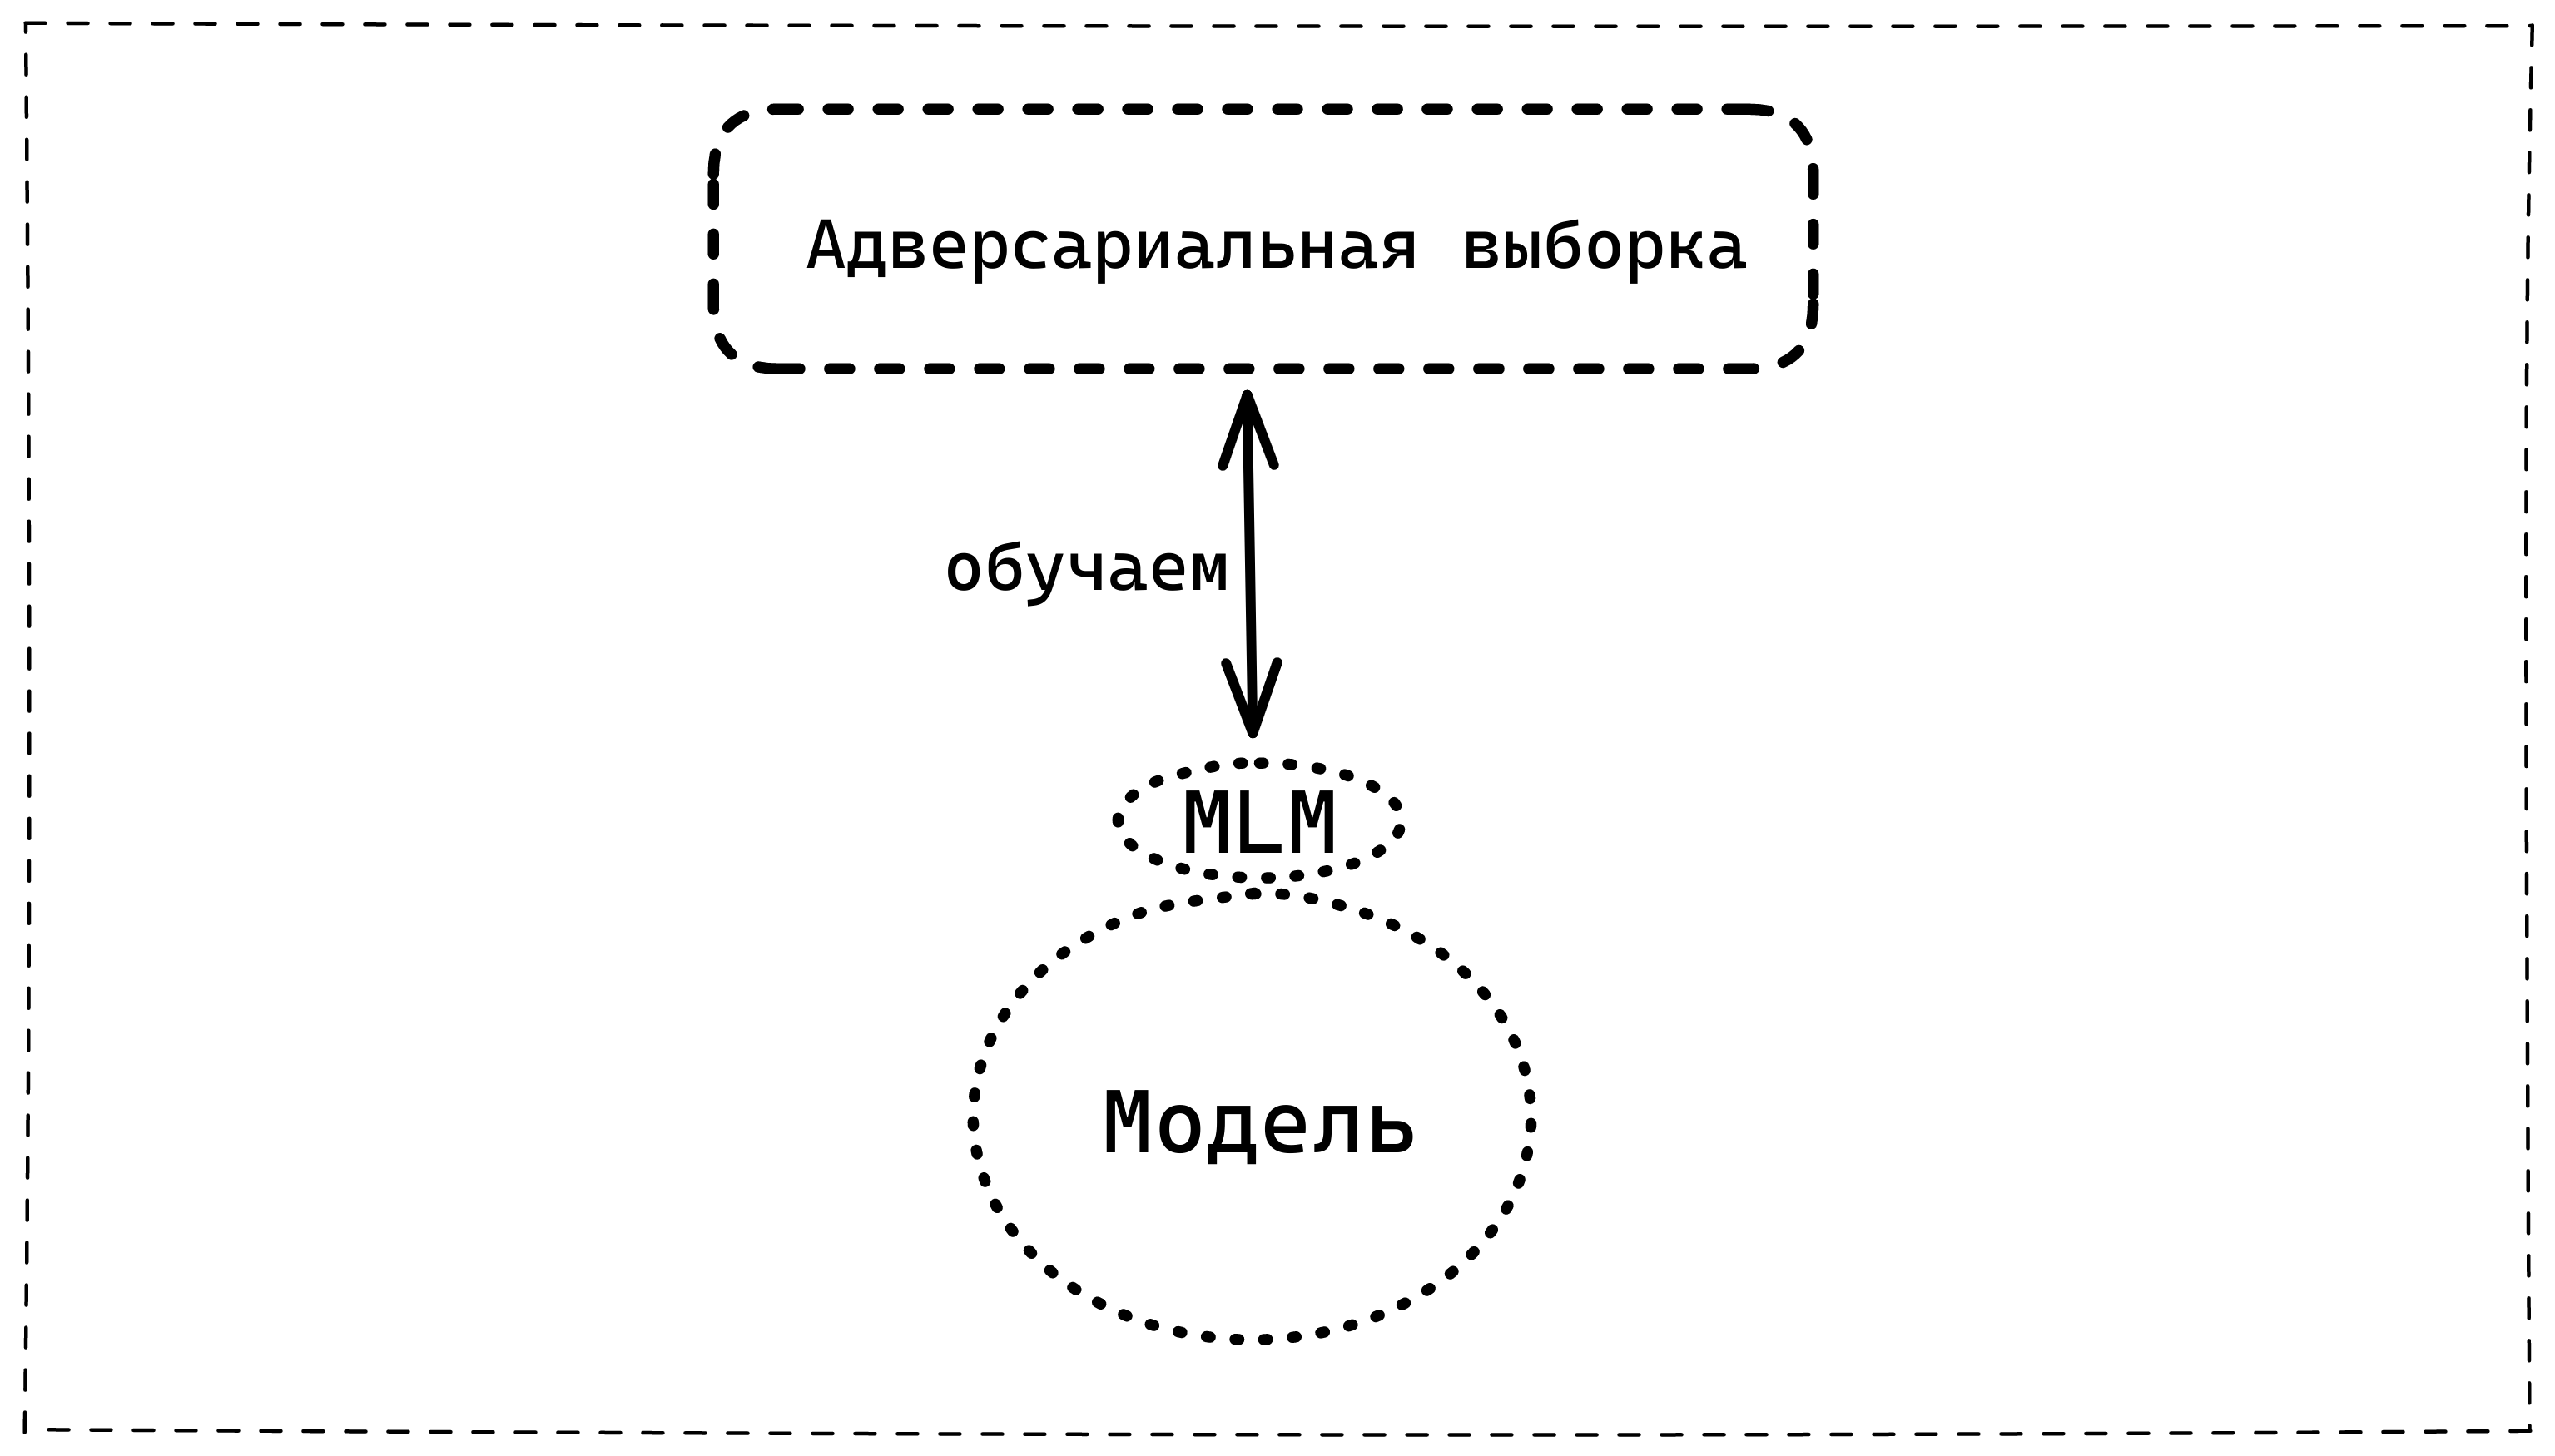
\includegraphics[width=\linewidth]{slides/10}\label{fig:figure28}
			\end{figure}
		\end{onlyenv}

		\begin{onlyenv}<3>
			\begin{figure}
				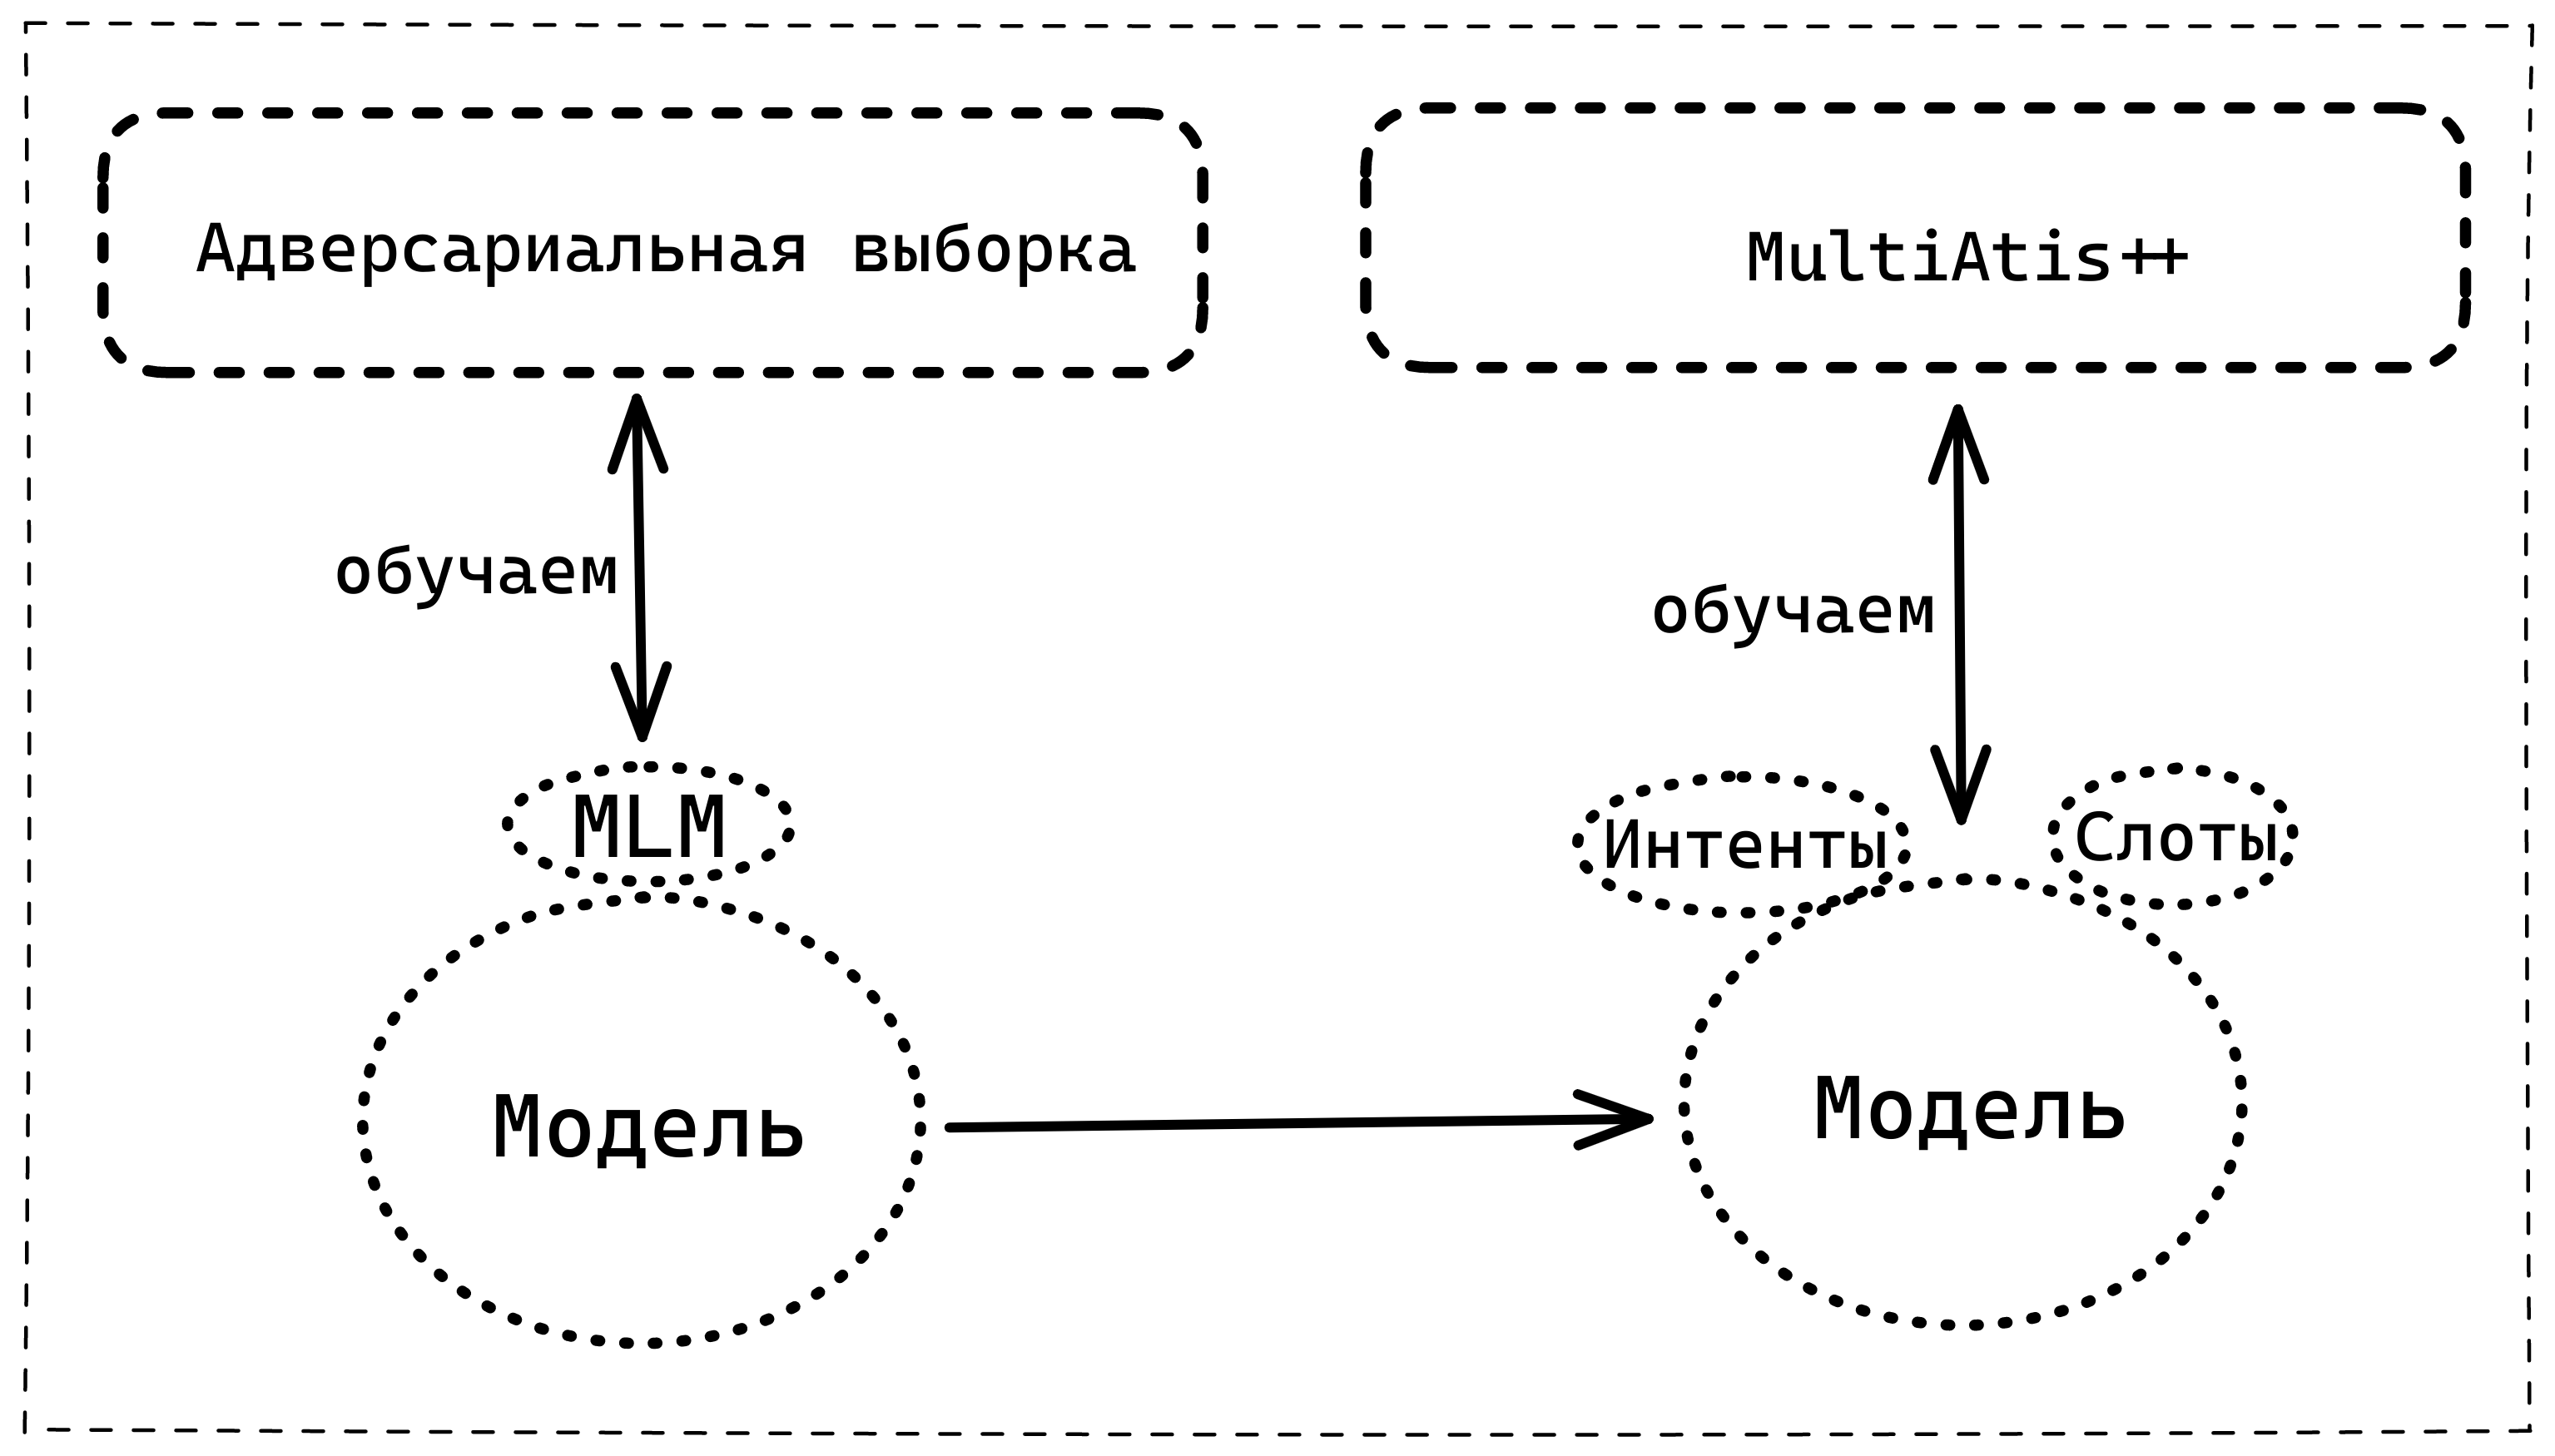
\includegraphics[width=\linewidth]{slides/11}\label{fig:figure29}
			\end{figure}
		\end{onlyenv}

		\note{Теперь я бы хотел рассказать про метод защиты от атак, который мы придумали. Это метод защиты от атак, которые имитируют смешение кодов. Предлагаемый метод состоит из двух шагов: Сначала мы генерируем выборку для задачи маскированного моделирования языка. Потом мы дообучаем тело модели на сгенерированной выборке. Полученное тело модели мы загружаем перед обучением в задаче классификации интентов и заполнения слотов.\newlineДля генерации выборки мы используем адаптацию phrase-level алгоритма атаки. Разница заключается в том, что замена токенов происходит случайно с вероятностью одна вторая. Мы по очереди встраиваем все шесть языков из нашего набора данных (кроме английского) в английскую обучающую выборку. Итоговая адверсариальная выборка является конкатенацией шести подвыборок.\newlineПосле генерации выборки мы используем ее для дообучения тела модели. Модель обучается в режиме маскированного моделирования языка. Для такой задачи мы в каждом входном батче отбираем 15\% токенов. 80\% отобранных токенов заменяются на токен маски, 10\% на случайные слова из словаря модели, остальные 10\% остаются неизменными, это стандартный процесс обучения моделей с архитектурой берта для задачи маскированного моделирования языка. После обучения мы загружаем модель и обучаемся для задачи классификации интентов и заполнения слотов.}
	\end{frame}

%------------------------------------------------


	\section{Результаты}
%------------------------------------------------

	\begin{frame}{Тестовая выборка}
		\begin{onlyenv}<1>
			\begin{figure}
				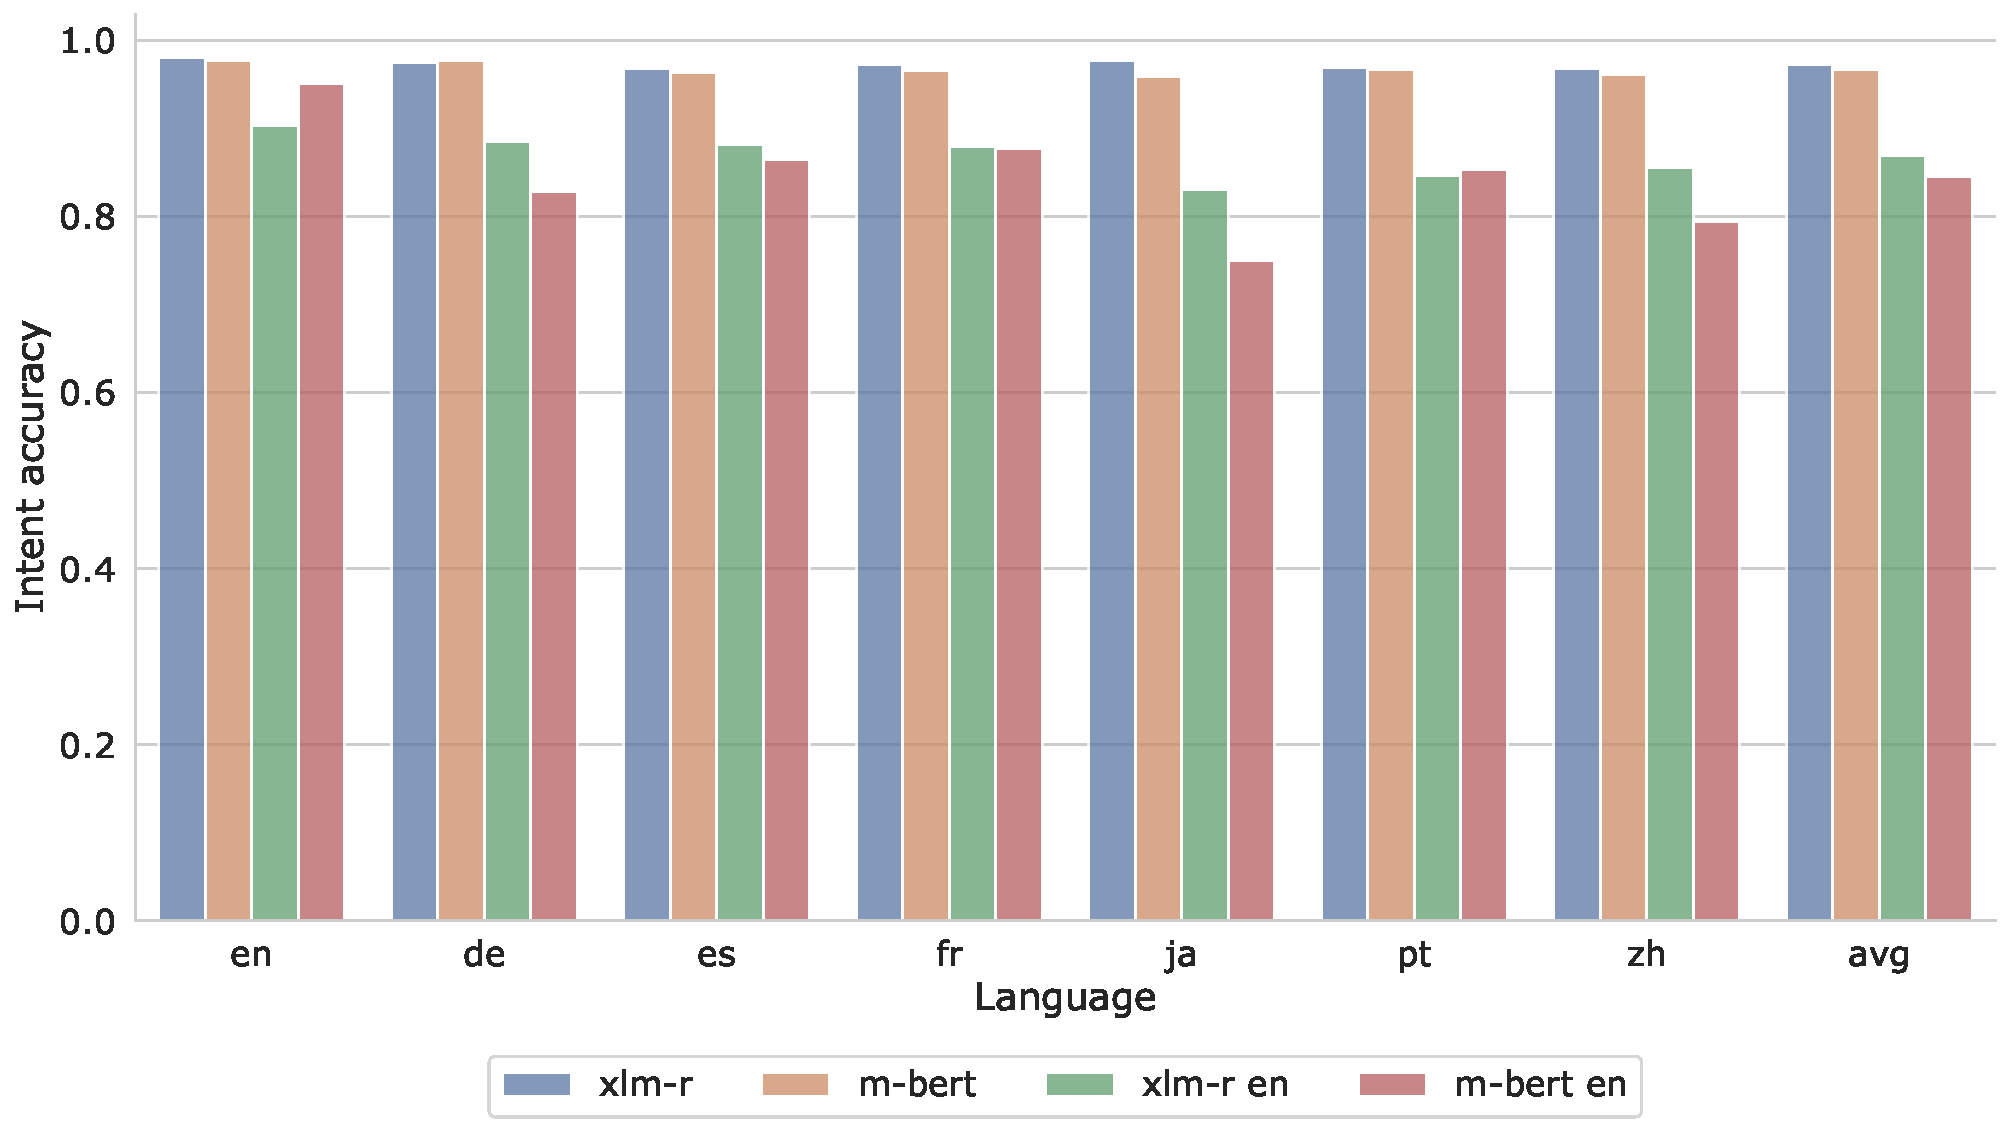
\includegraphics[width=0.9\linewidth]{images/0}\label{fig:figure10}\caption*{Доля предложений с верно классифицированным интентом}
			\end{figure}
		\end{onlyenv}

		\begin{onlyenv}<2>
			\begin{figure}
				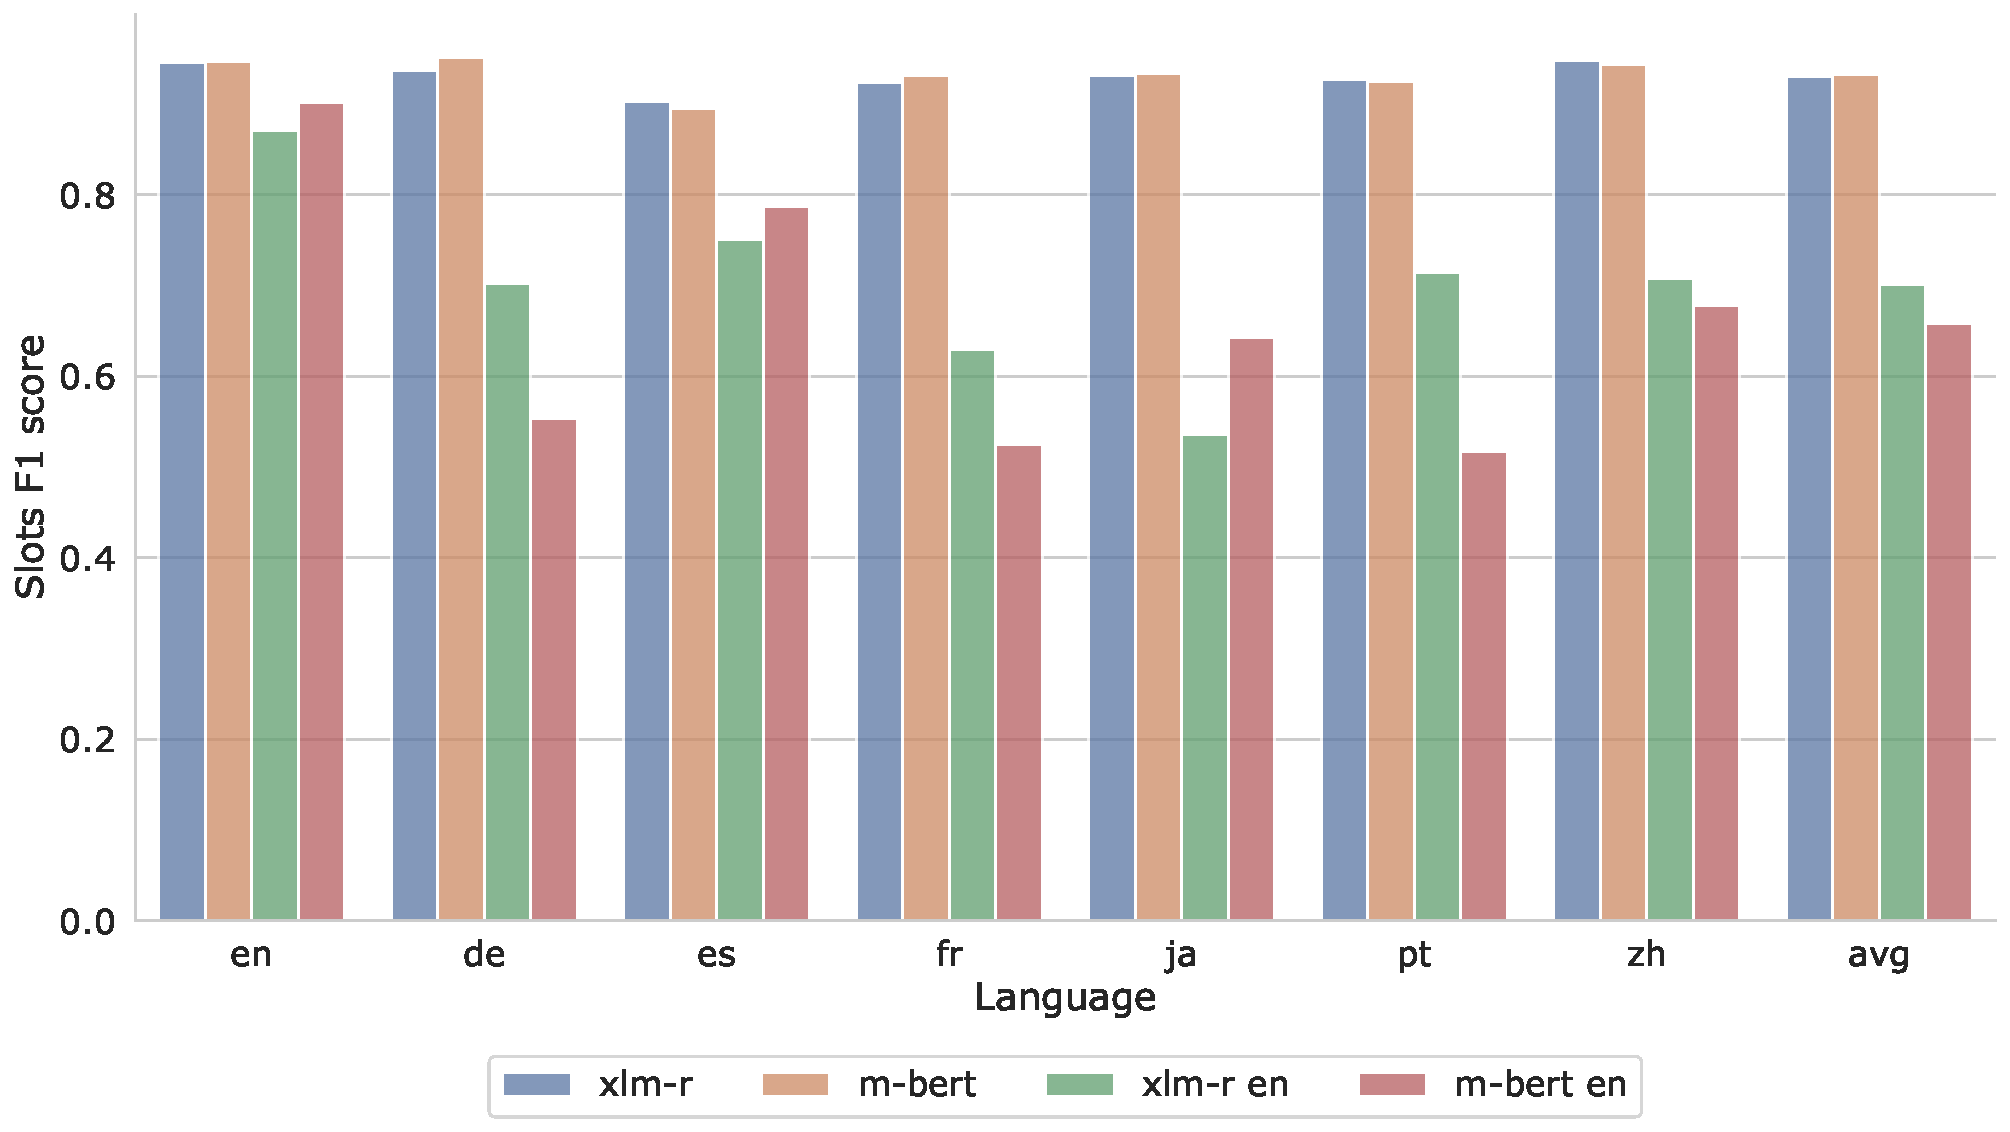
\includegraphics[width=0.9\linewidth]{images/1}\label{fig:figure11}\caption*{F1 мера по слотам}
			\end{figure}
		\end{onlyenv}

		\begin{onlyenv}<3>
			\begin{figure}
				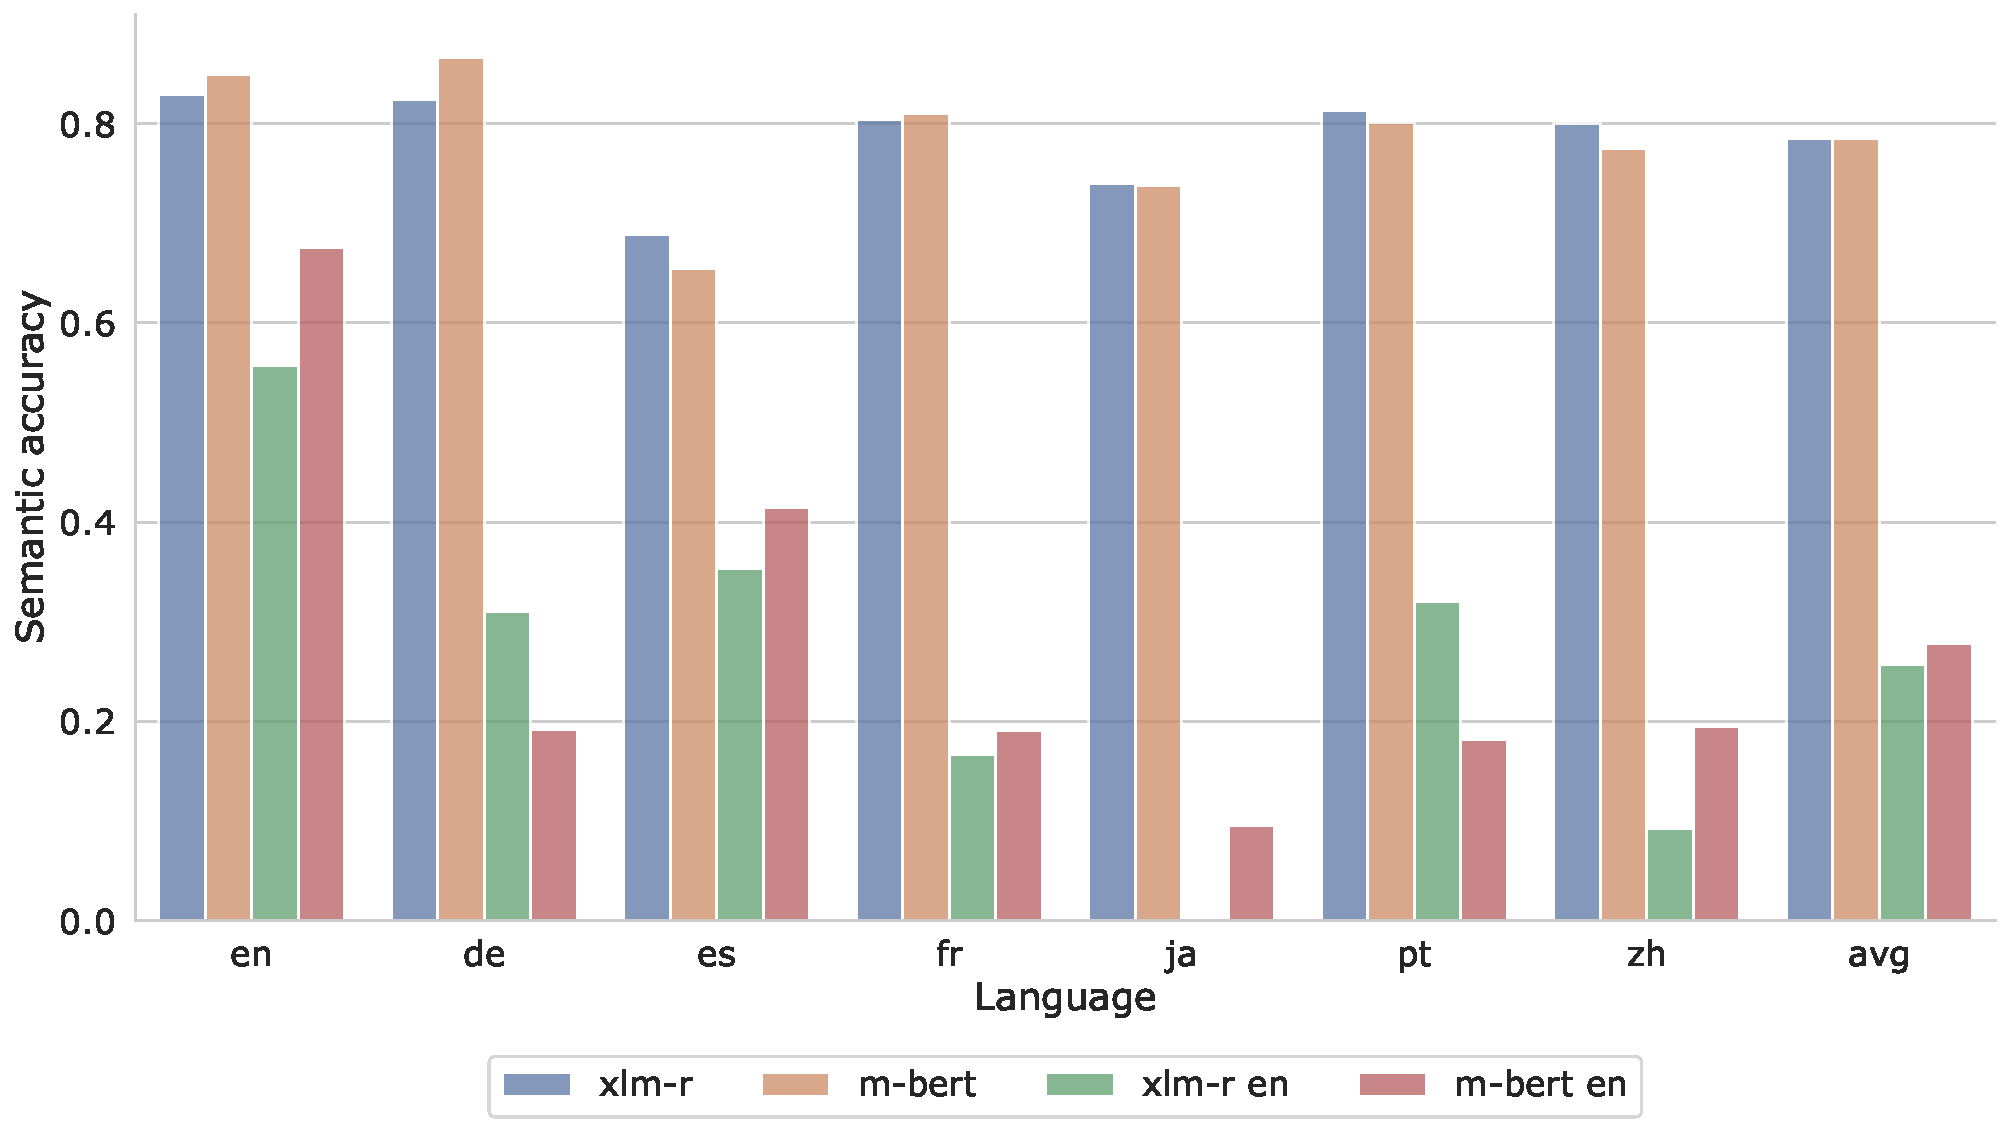
\includegraphics[width=0.9\linewidth]{images/2}\label{fig:figure12}\caption*{Доля полностью верно классифицированных предложений}
			\end{figure}
		\end{onlyenv}

		\note{Перед тем как приступить к рассказу про результаты я бы хотел рассказать какие модели мы будем сравнивать и по каким метрикам. Мы будем сравнивать модели, обученные только на английской обучающей выборке (слабые модели) и на полной обучающей выборке (сильные модели). Оценивать качество мы будем по трём метрикам - доля предложений, где мы верно классифицировали интент, f1 мера по слотам (мы использовали микро-усреднение по классам) и доля предложений, где мы верно классифицировали вообще всё - и интент и все слоты.\newlineПриступим к обсуждению результатов.\newlineМы успешно решили задачу классификации интентов и заполнения слотов. Сильные модели показали на тестовой выборке в среднем 97\% правильных ответов по интентам, слабые в среднем 85\%. Сильные модели показали 0.93 f1 меры по слотам, слабые 0.68. Сильные модели показали 79\% полностью верно классифицированных предложений, а слабые около 26\%. Мы обнаружили, что слабые модели имеют ощутимо худшее качество, чем сильные, причем не только на других языках кроме английского, но и даже на английском.}
	\end{frame}

	\begin{frame}{Word-level атака}
		\begin{onlyenv}<1>
			\begin{figure}
				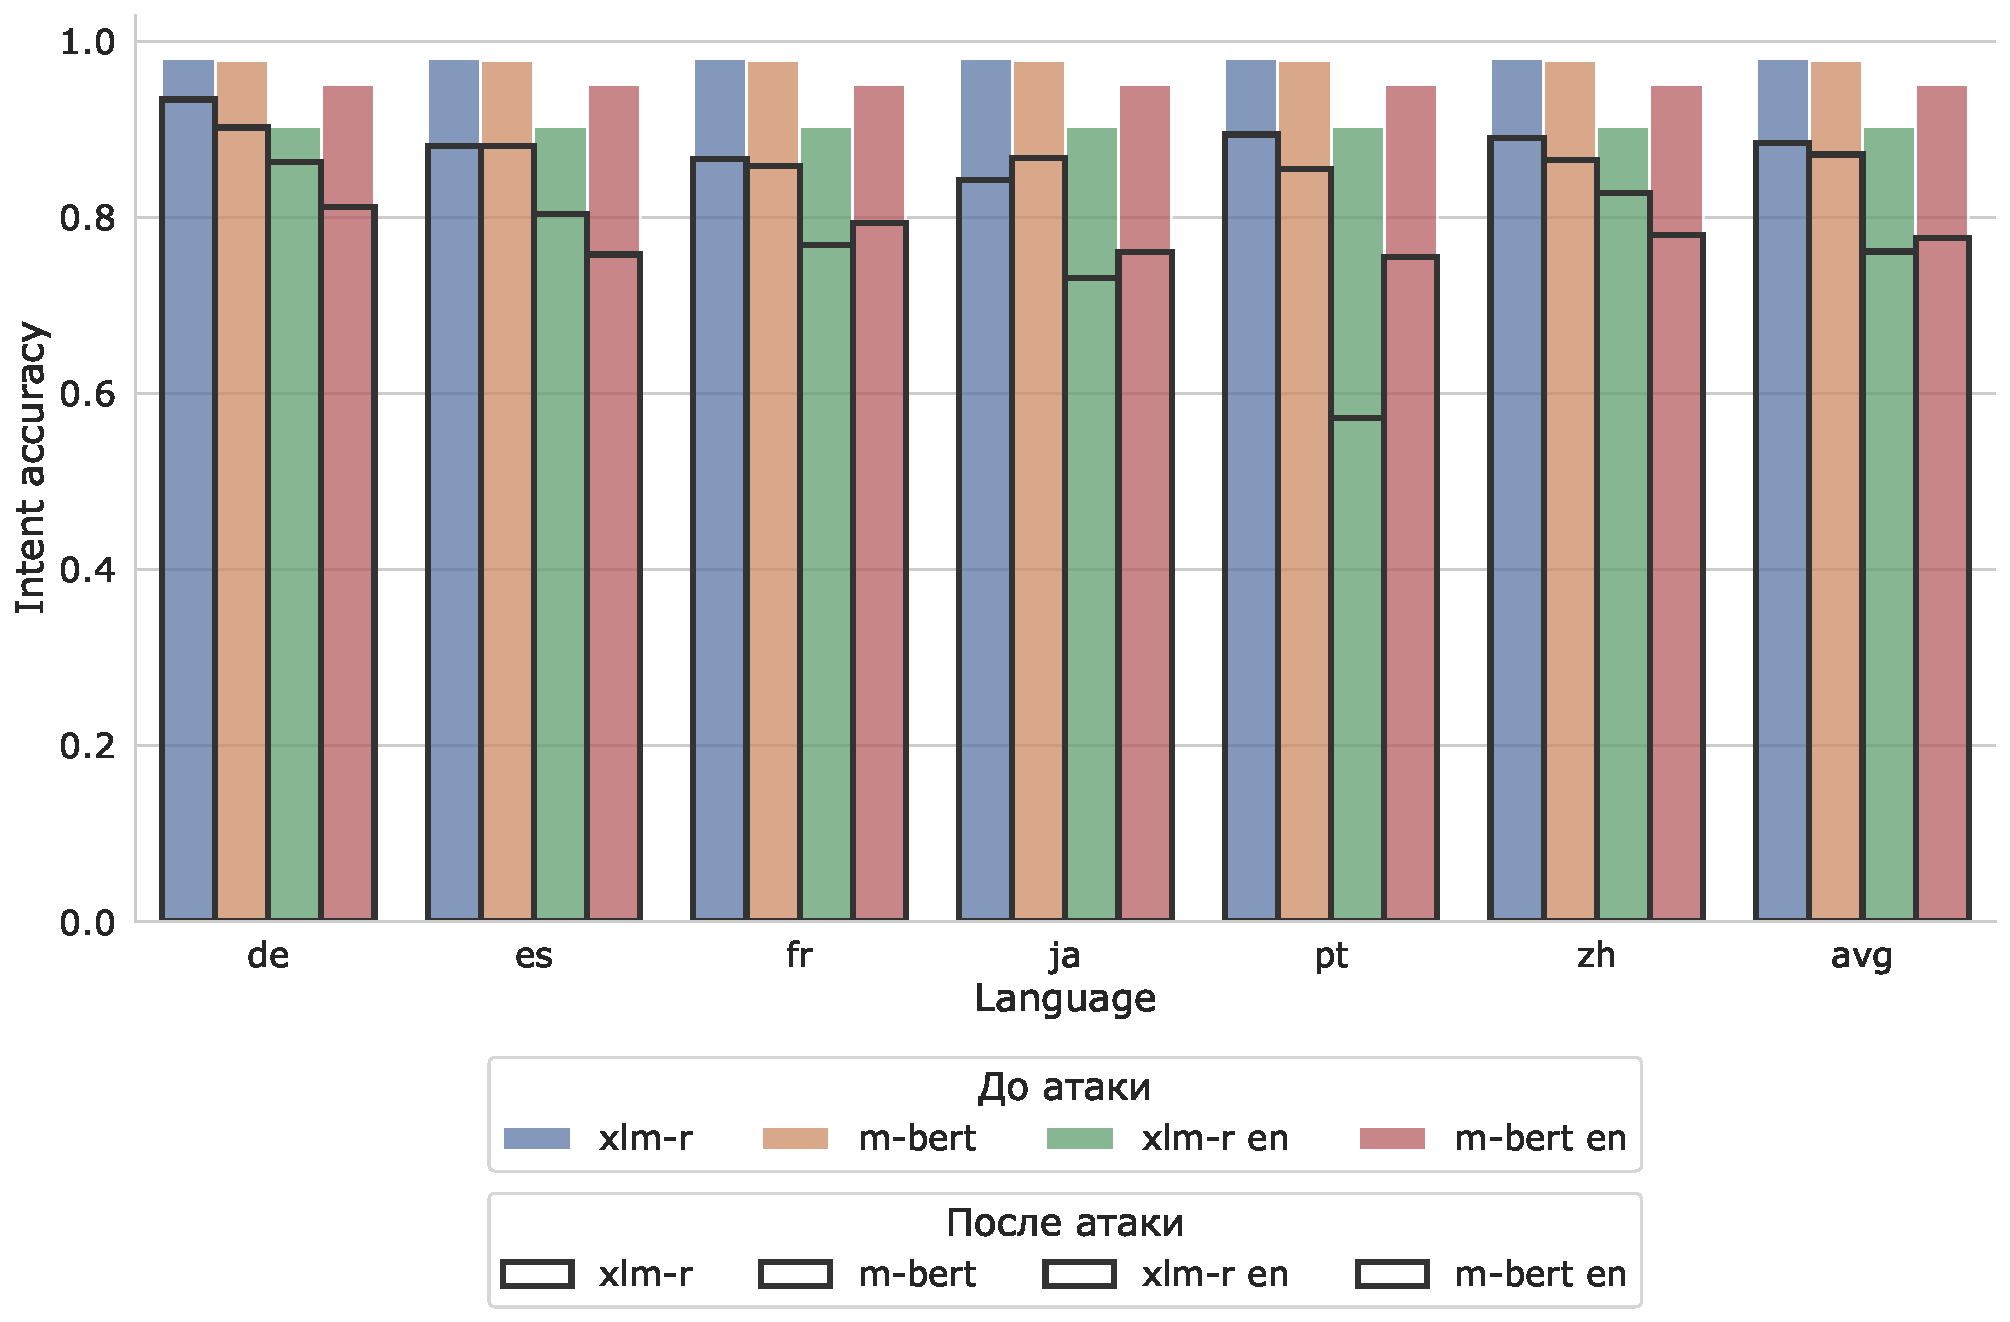
\includegraphics[width=0.9\linewidth]{images/3}\label{fig:figure13}\caption*{Доля предложений с верно классифицированным интентом}
			\end{figure}
		\end{onlyenv}

		\begin{onlyenv}<2>
			\begin{figure}
				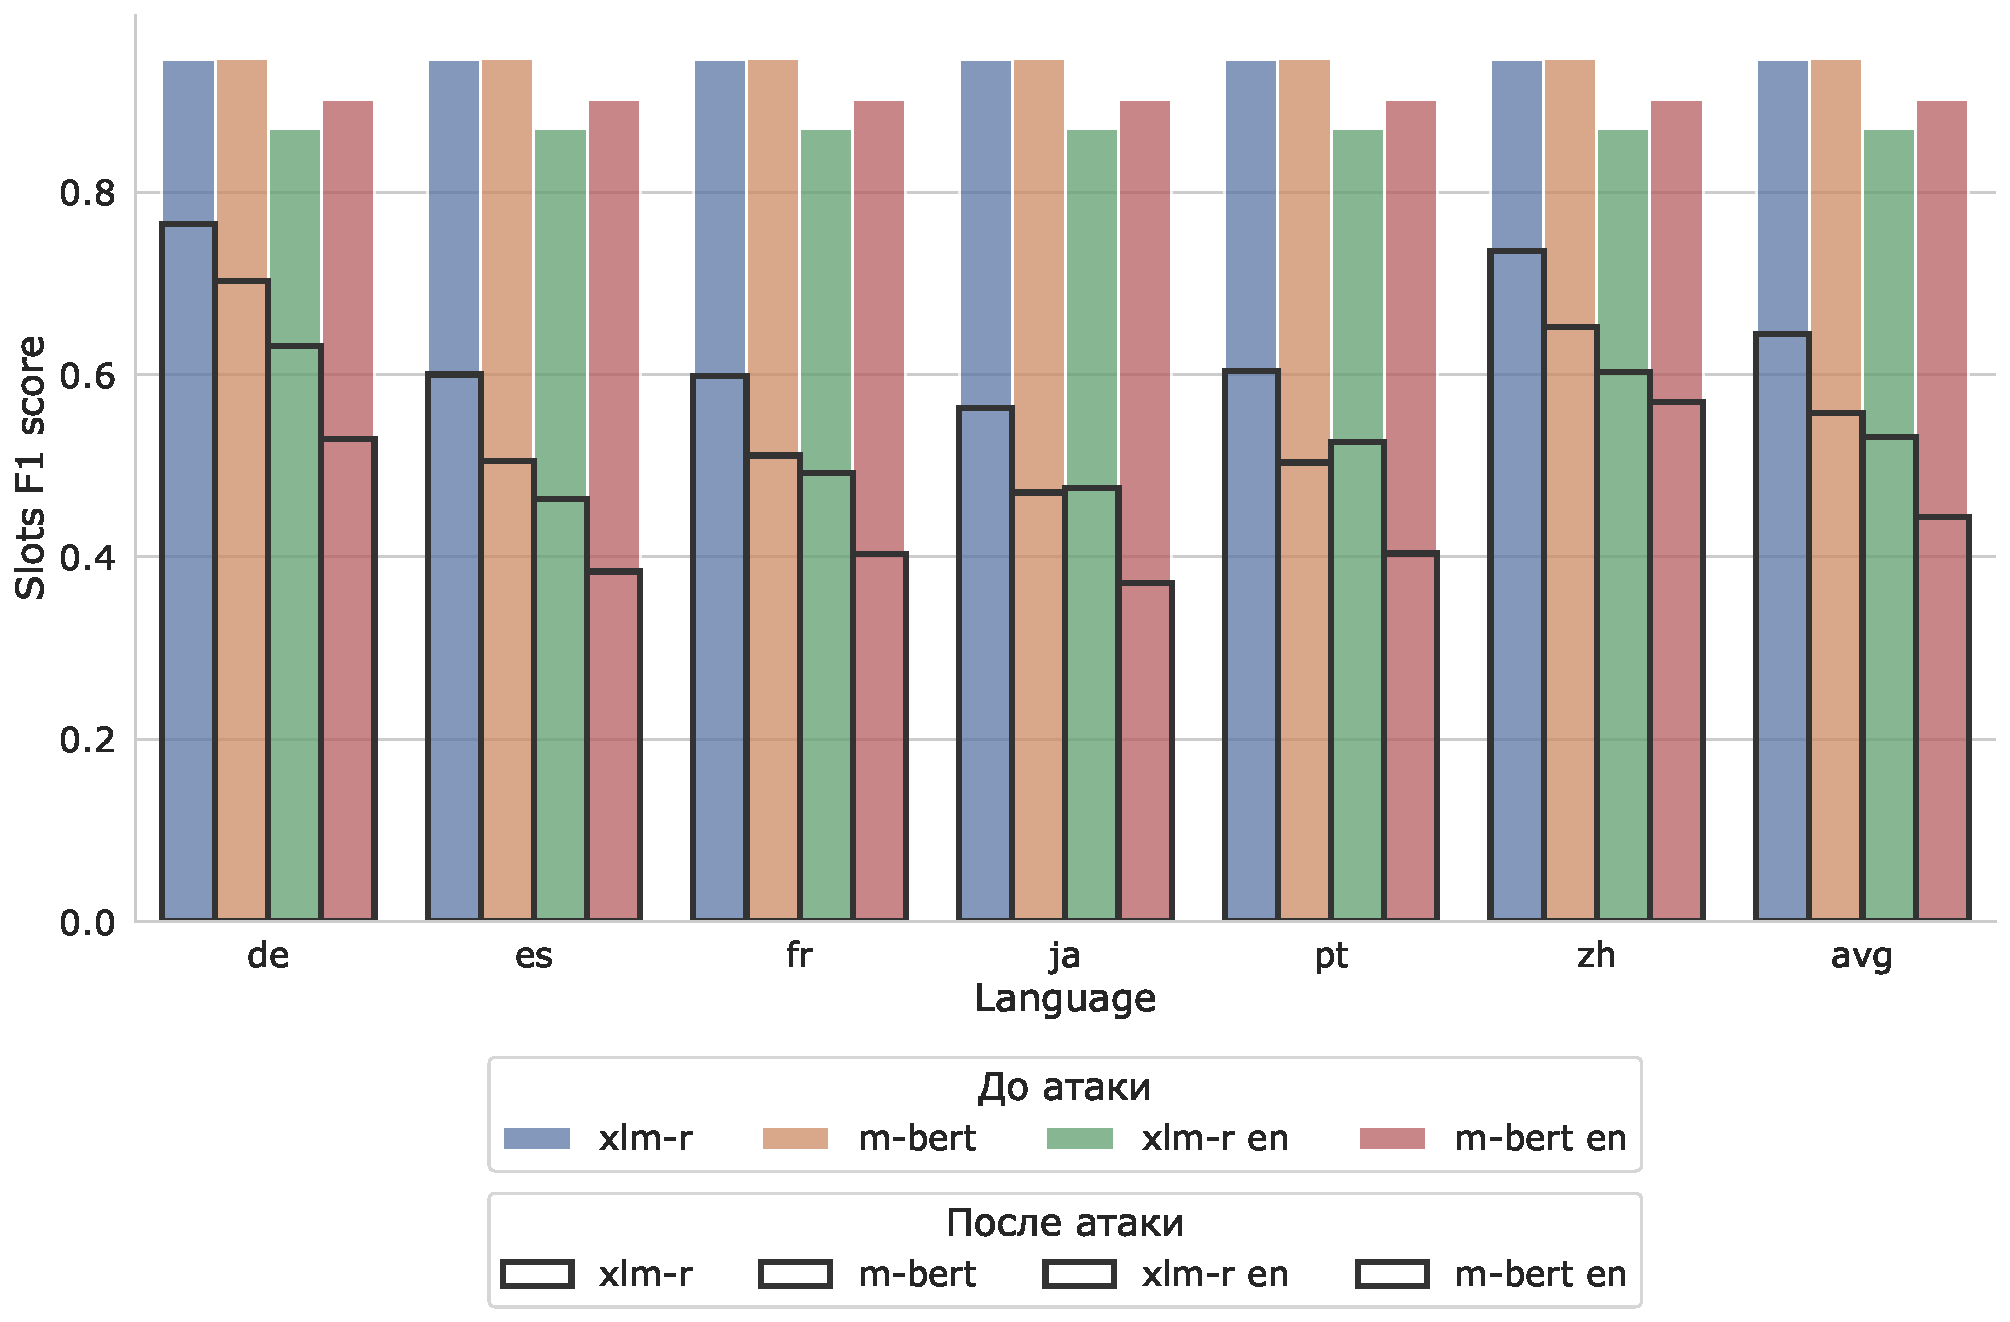
\includegraphics[width=0.9\linewidth]{images/4}\label{fig:figure14}\caption*{F1 мера по слотам}
			\end{figure}
		\end{onlyenv}

		\begin{onlyenv}<3>
			\begin{figure}
				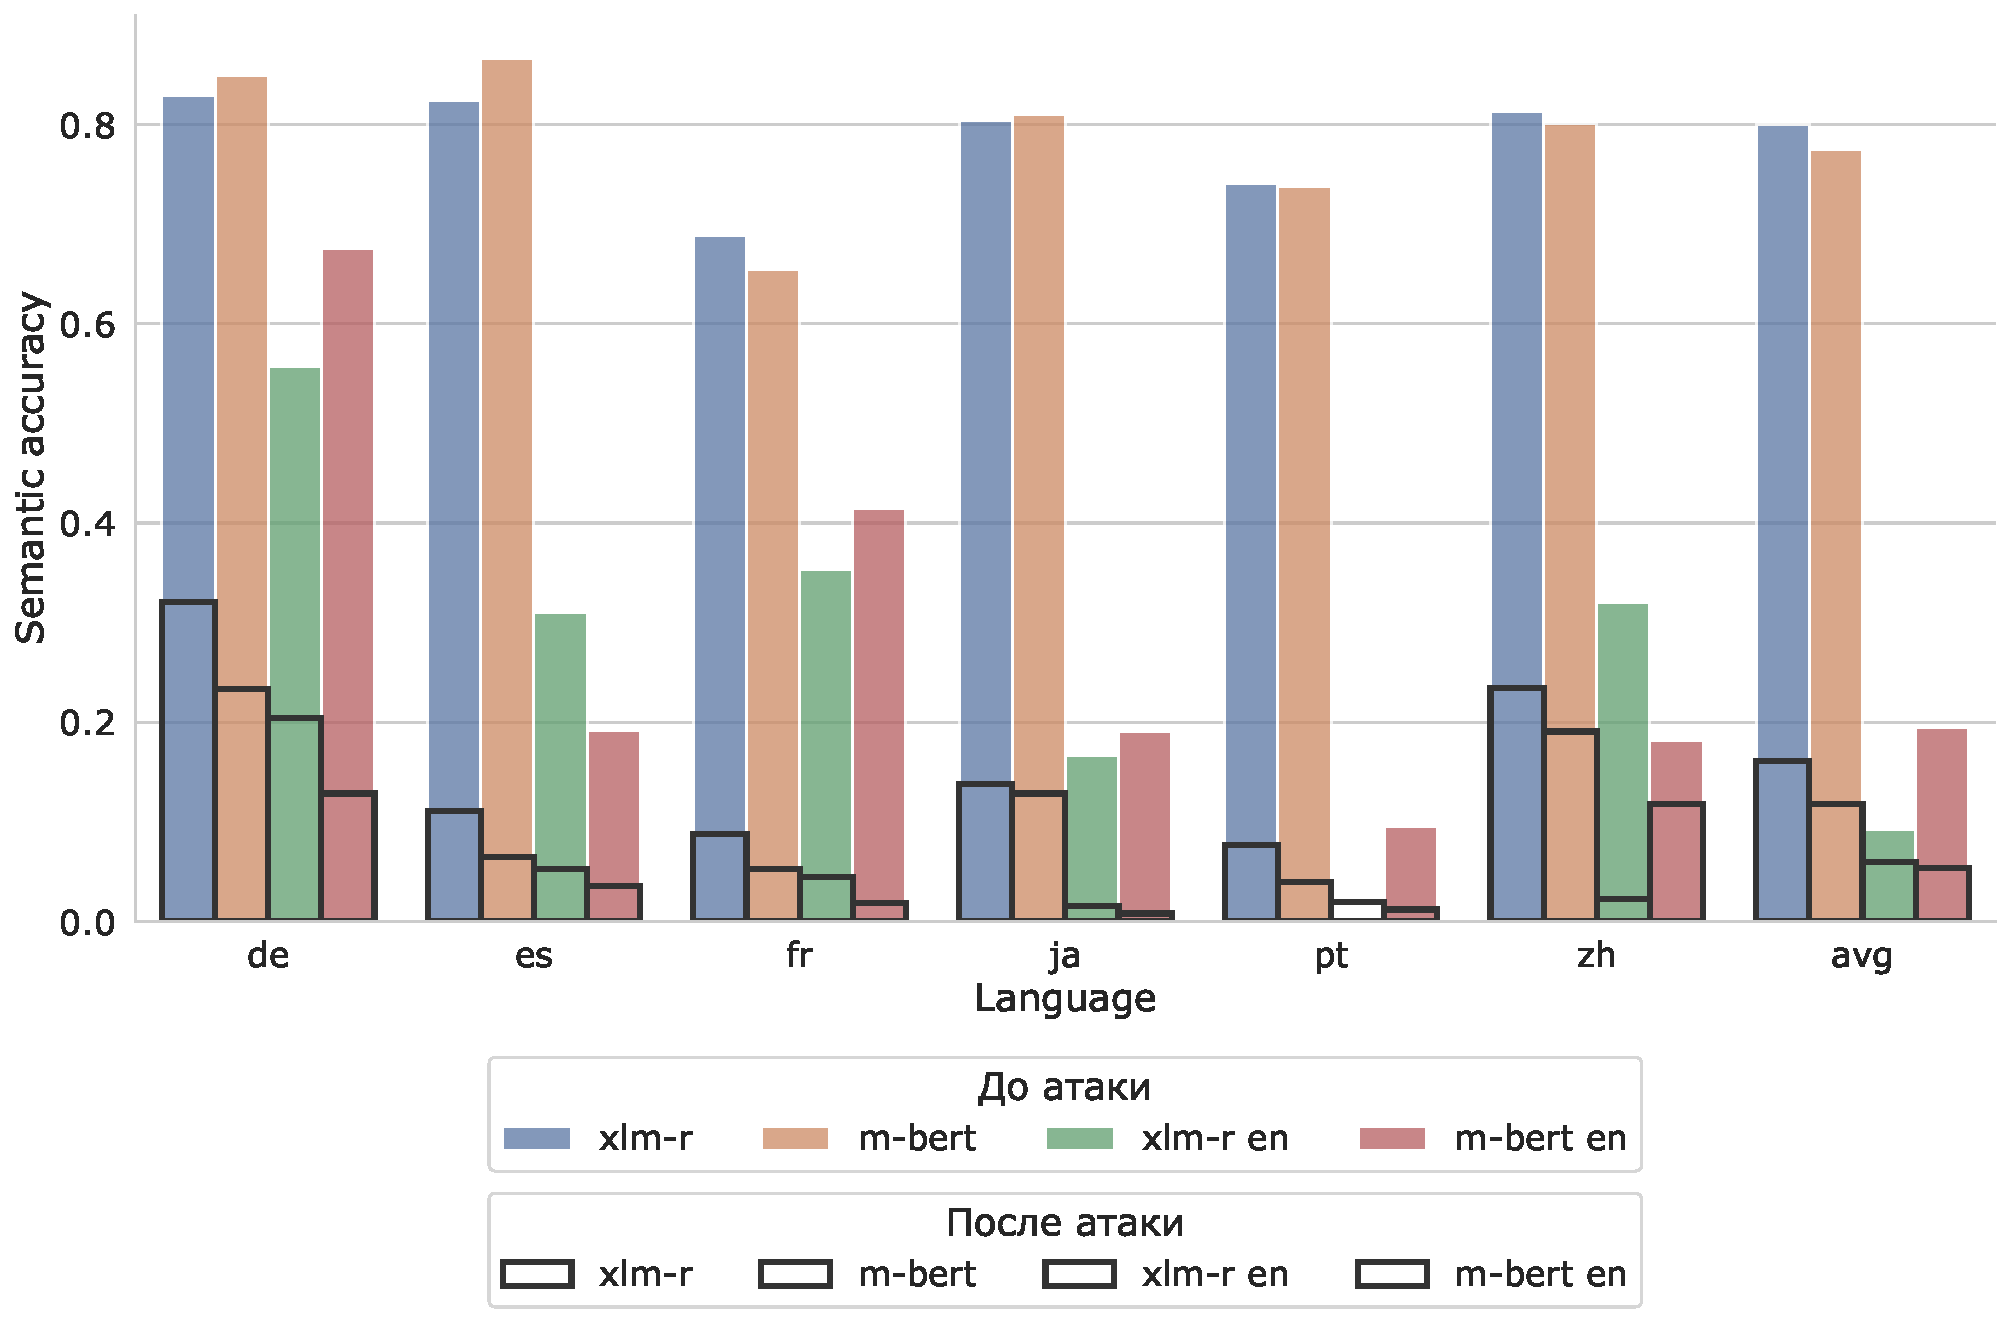
\includegraphics[width=0.9\linewidth]{images/5}\label{fig:figure15}\caption*{Доля полностью верно классифицированных предложений}
			\end{figure}
		\end{onlyenv}


		\note{Мы проатаковали все модели с помощью наших двух алгоритмов.\newlineМы получили, что word-level атака получилась сильной атакой и дала низкое качество. У сильных моделей качество по интентам упало с 98 до 88\%, у слабых с 92 до 77\%. У сильных моделей качество по слотам упало с 0.95 до 0.6, у слабых с 0.88 до 0.48. У сильных моделей доля полностью верно классифицированных предложений упала с 83 до 14\%, у слабых с 60 до 5\%.}
	\end{frame}

	\begin{frame}{Phrase-level атака}
		\begin{onlyenv}<1>
			\begin{figure}
				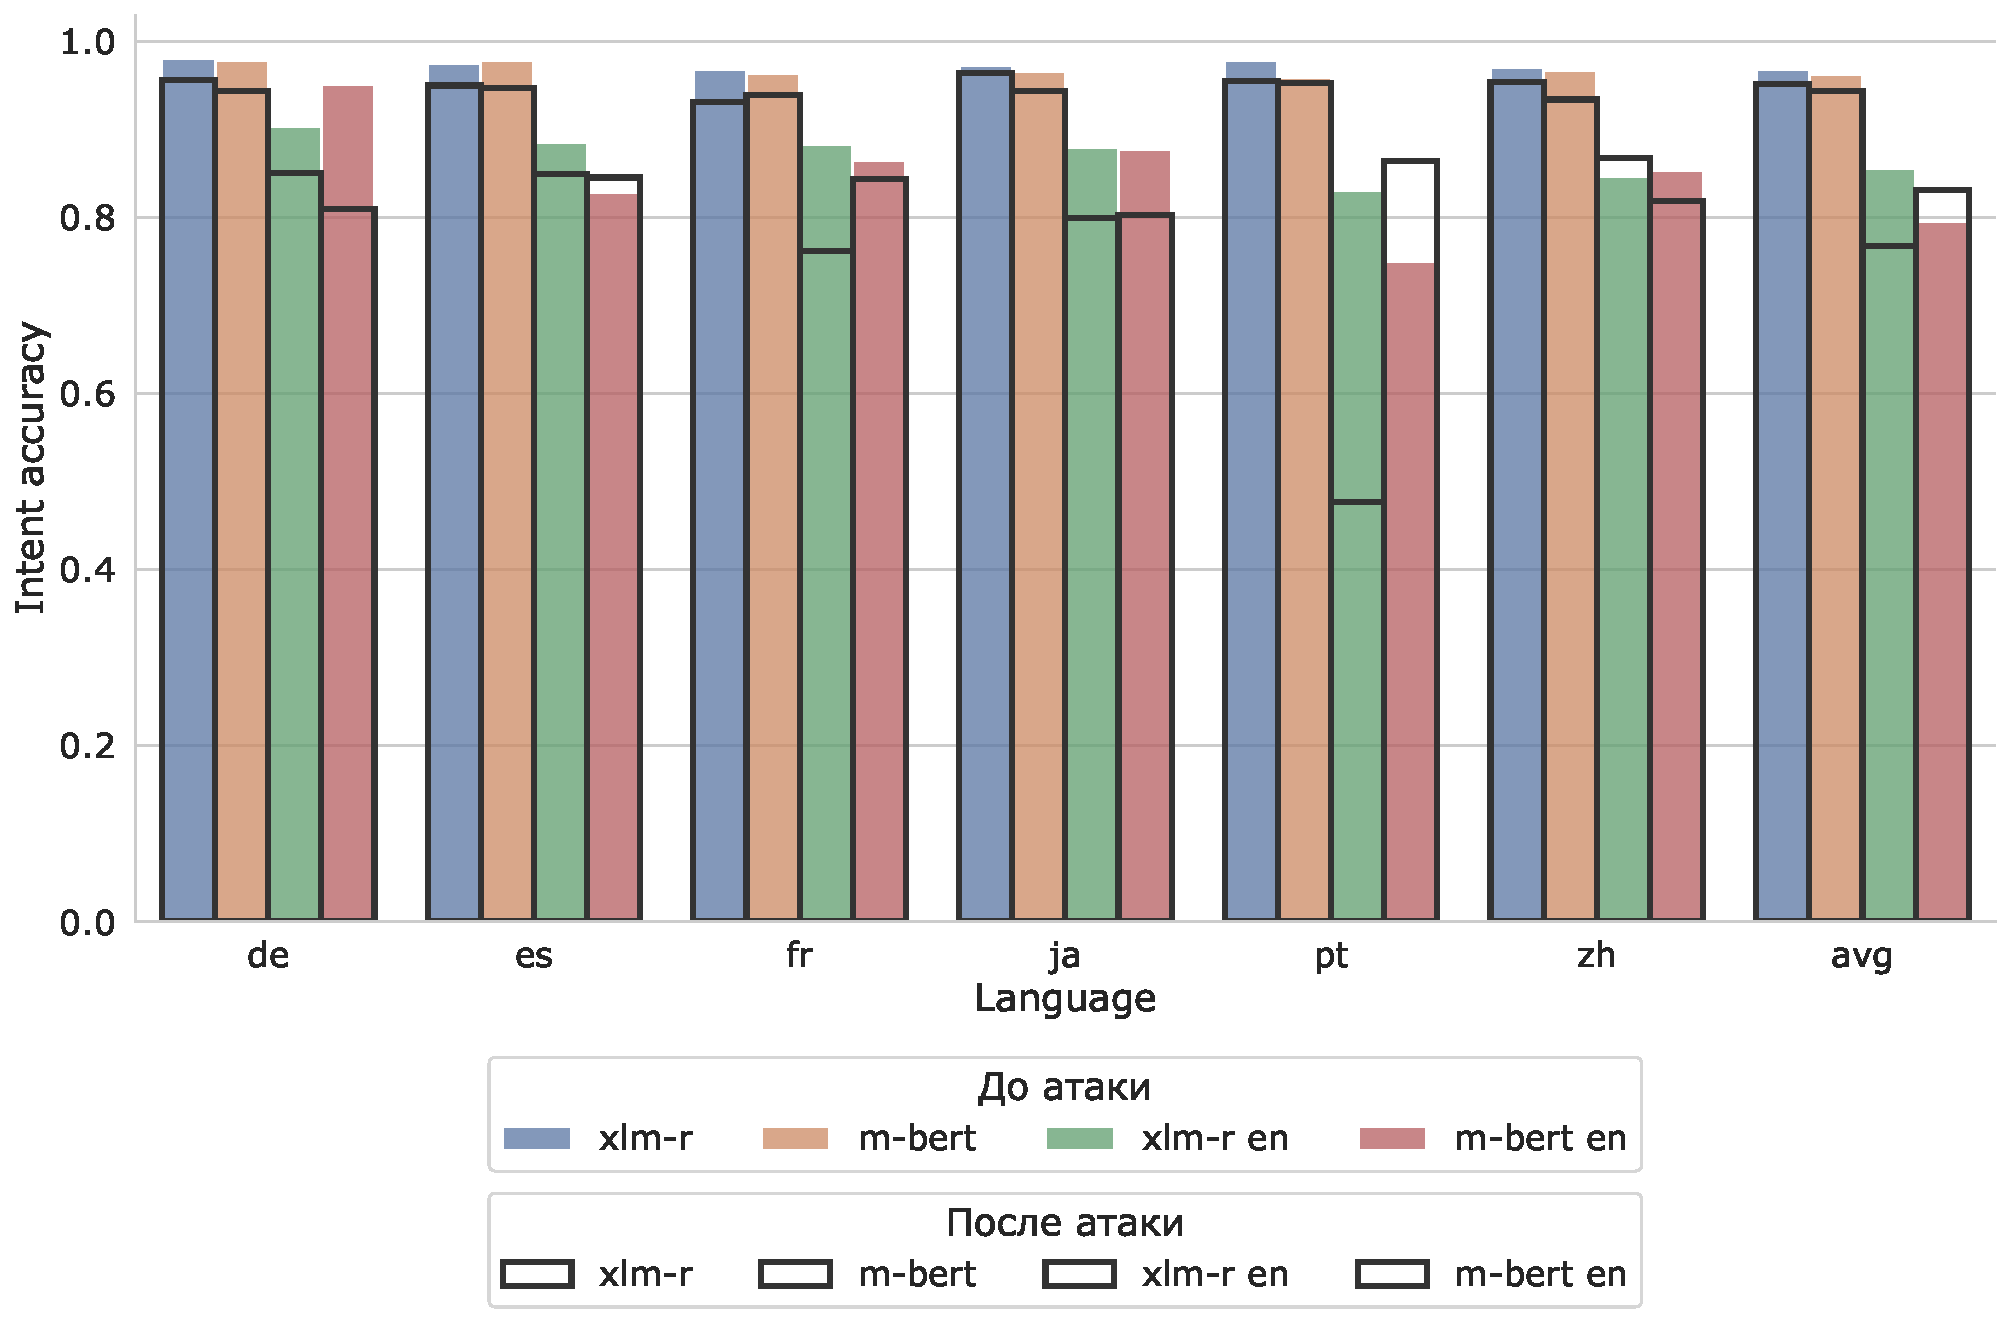
\includegraphics[width=0.9\linewidth]{images/6}\label{fig:figure16}\caption*{Доля предложений с верно классифицированным интентом}
			\end{figure}
		\end{onlyenv}

		\begin{onlyenv}<2>
			\begin{figure}
				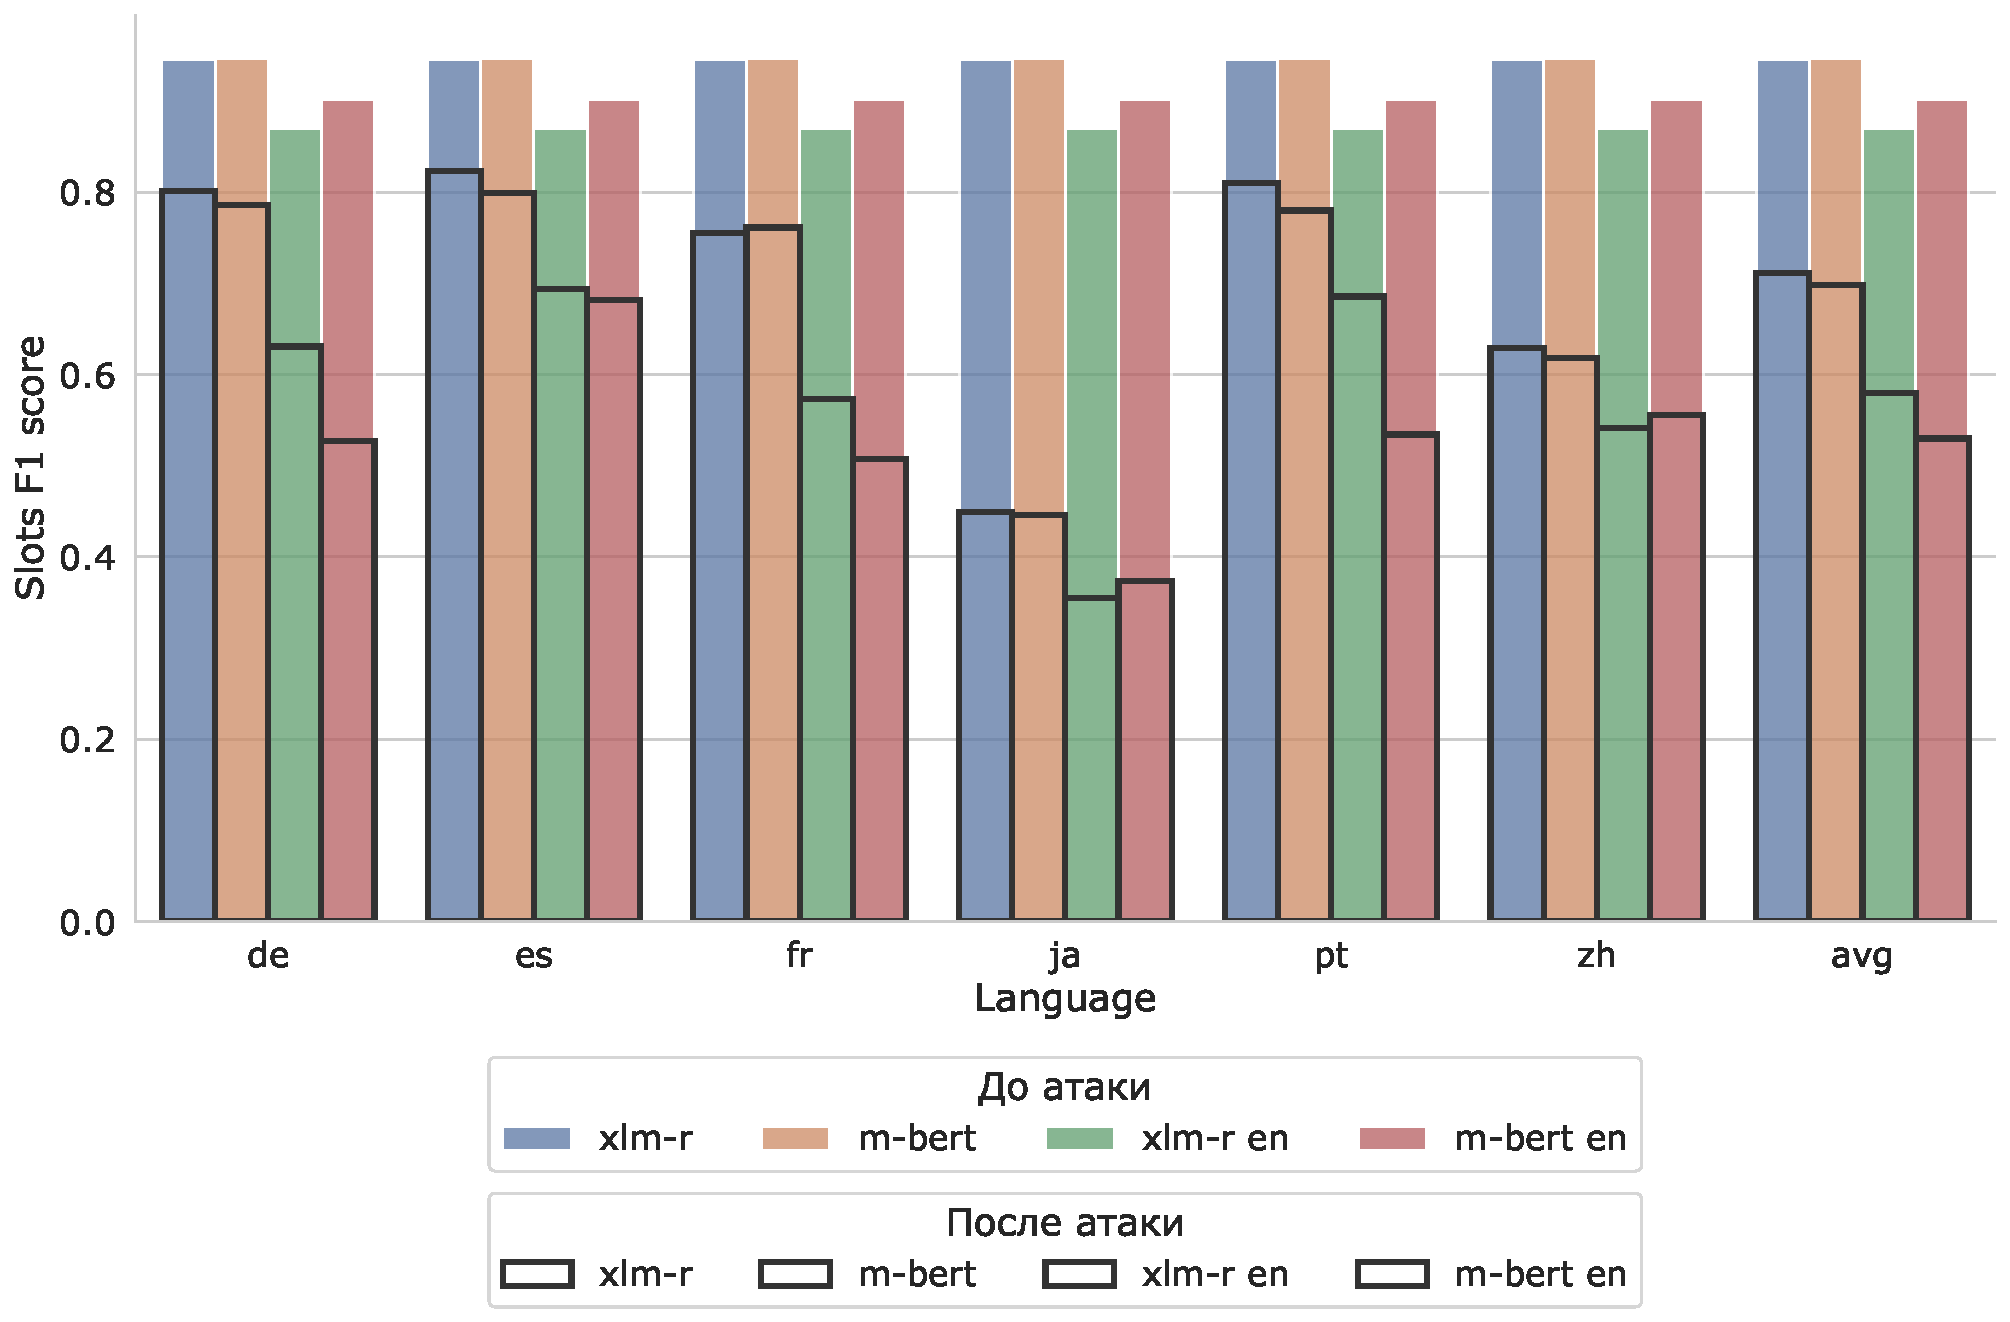
\includegraphics[width=0.9\linewidth]{images/7}\label{fig:figure17}\caption*{F1 мера по слотам}
			\end{figure}
		\end{onlyenv}

		\begin{onlyenv}<3>
			\begin{figure}
				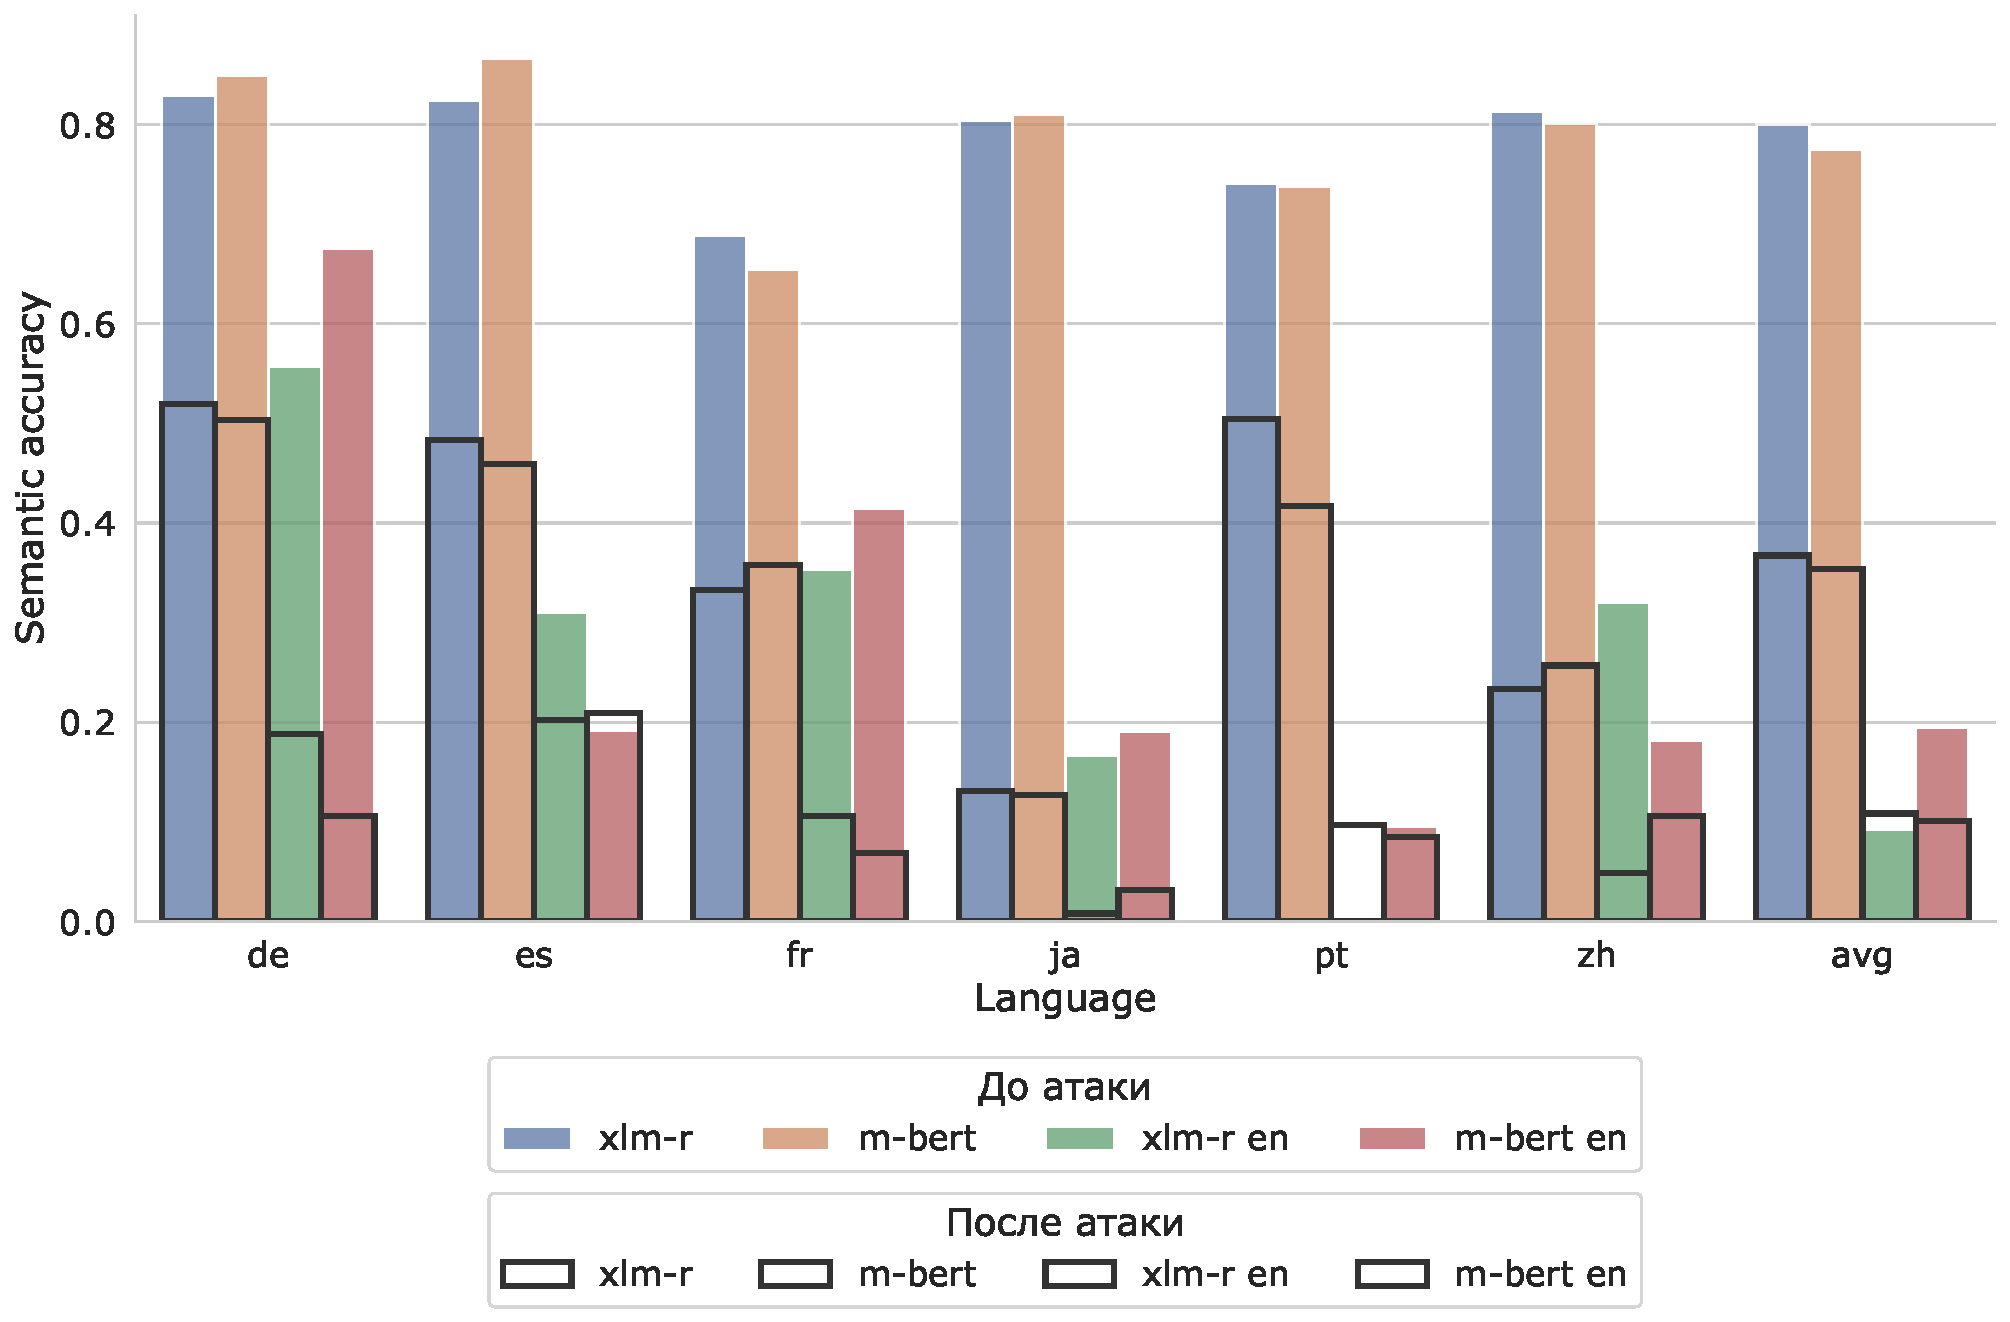
\includegraphics[width=0.9\linewidth]{images/8}\label{fig:figure18}\caption*{Доля полностью верно классифицированных предложений}
			\end{figure}
		\end{onlyenv}

		\note{Также мы получили, что phrase-level атака получилась более мягкой и дала более высокое качество по сравнению с word-level. У сильных моделей качество по интентам упало с 98 до 95\%, у слабых с  92 до 80\%. У сильных моделей качество по слотам упало с 0.95 до 0.7, у слабых с 0.88 до 0.55. У сильных моделей доля полностью верно классифицированных предложений упала с 83 до 35\%, у слабых с 60 до 10\%.}
	\end{frame}

	\begin{frame}{Тестовая выборка (с защитой)}
		\begin{onlyenv}<1>
			\begin{figure}
				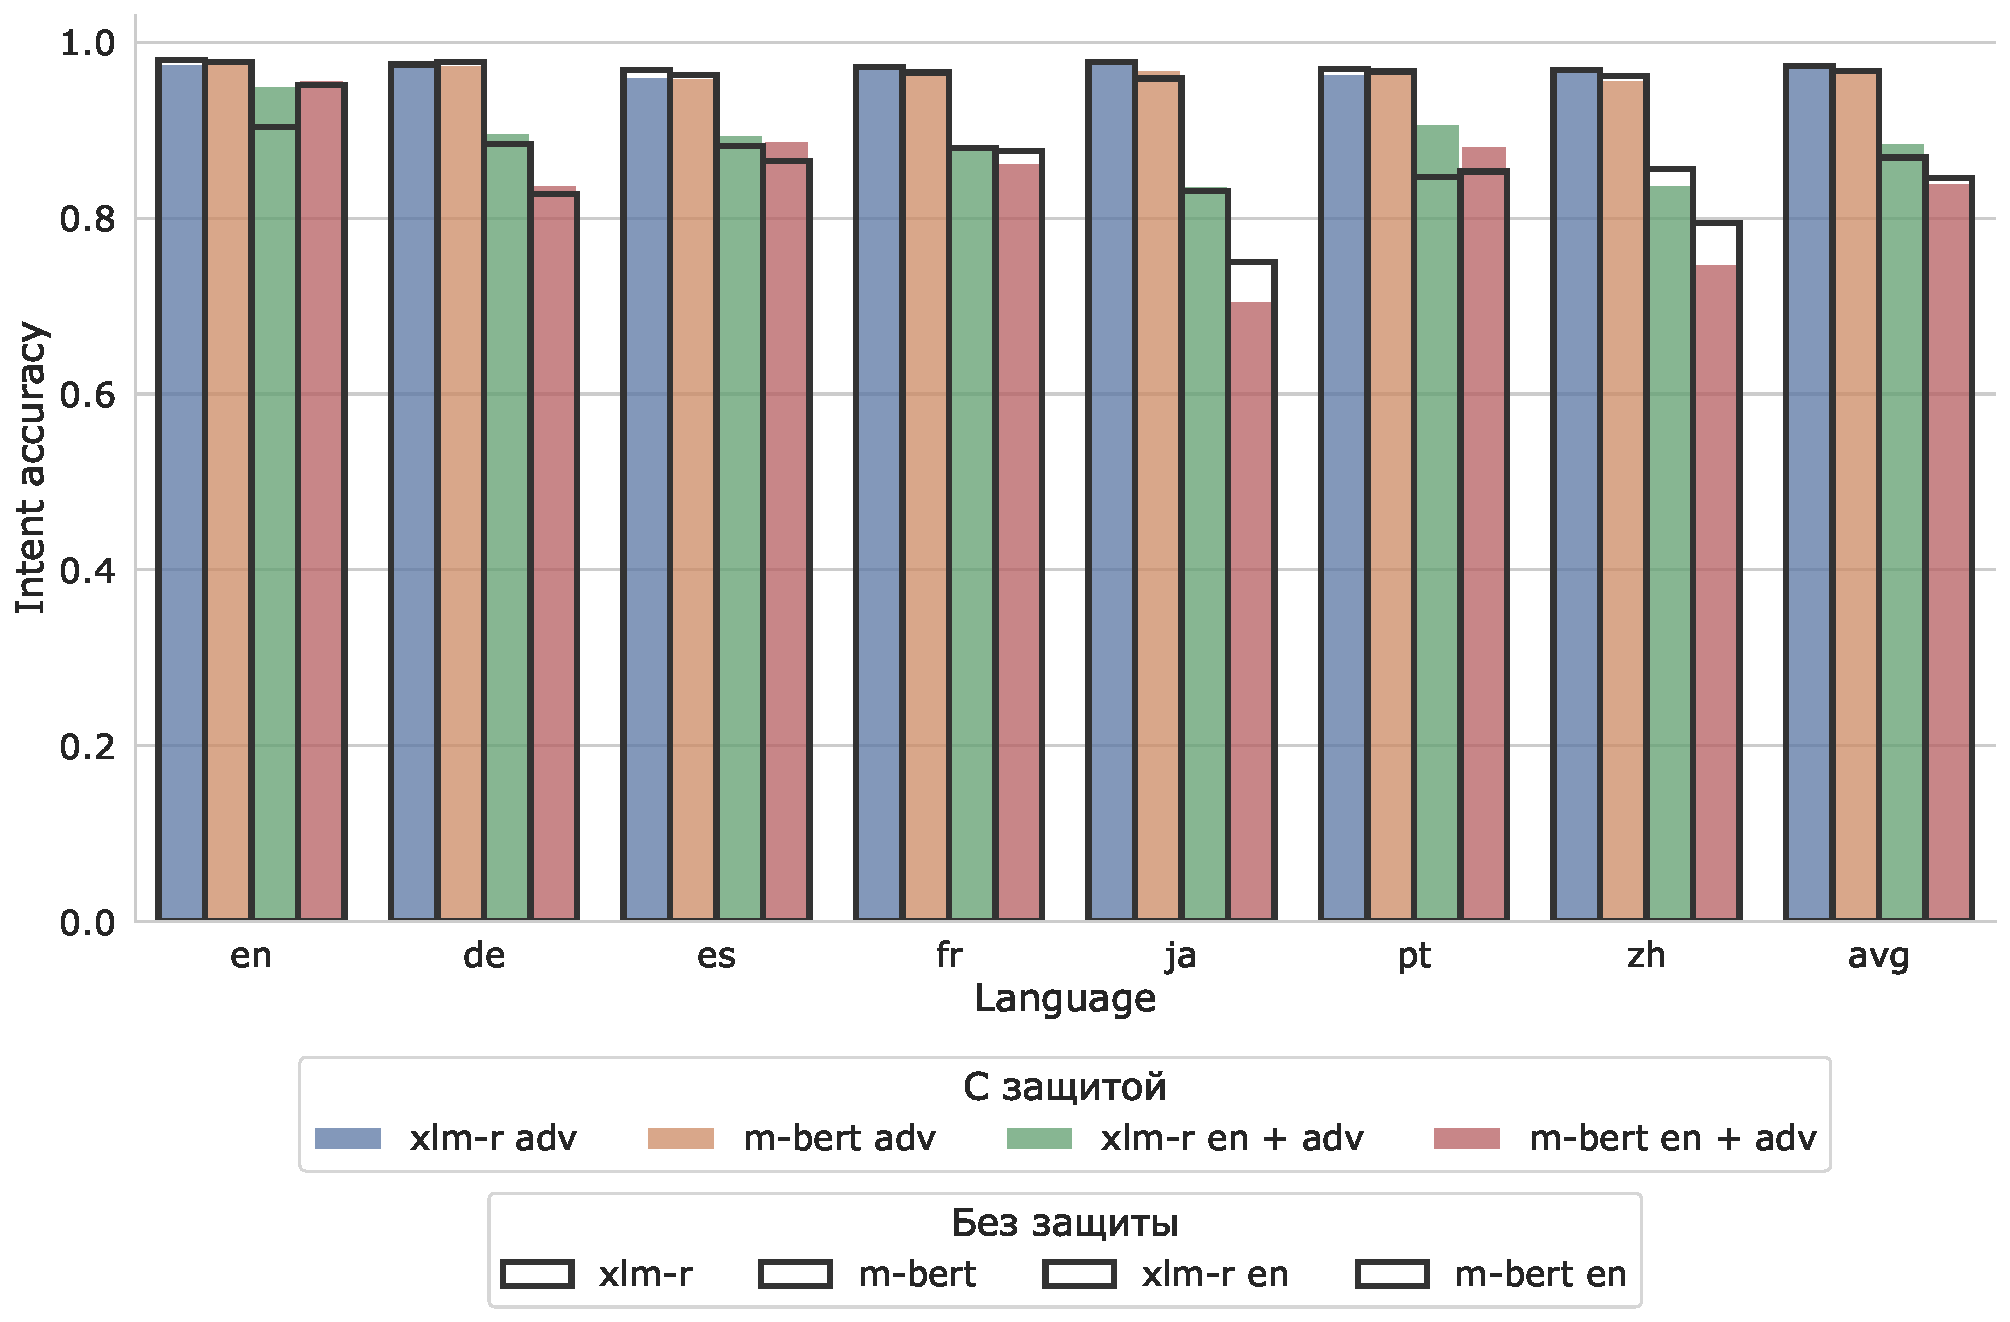
\includegraphics[width=0.9\linewidth]{images/9}\label{fig:figure19}\caption*{Доля предложений с верно классифицированным интентом}
			\end{figure}
		\end{onlyenv}

		\begin{onlyenv}<2>
			\begin{figure}
				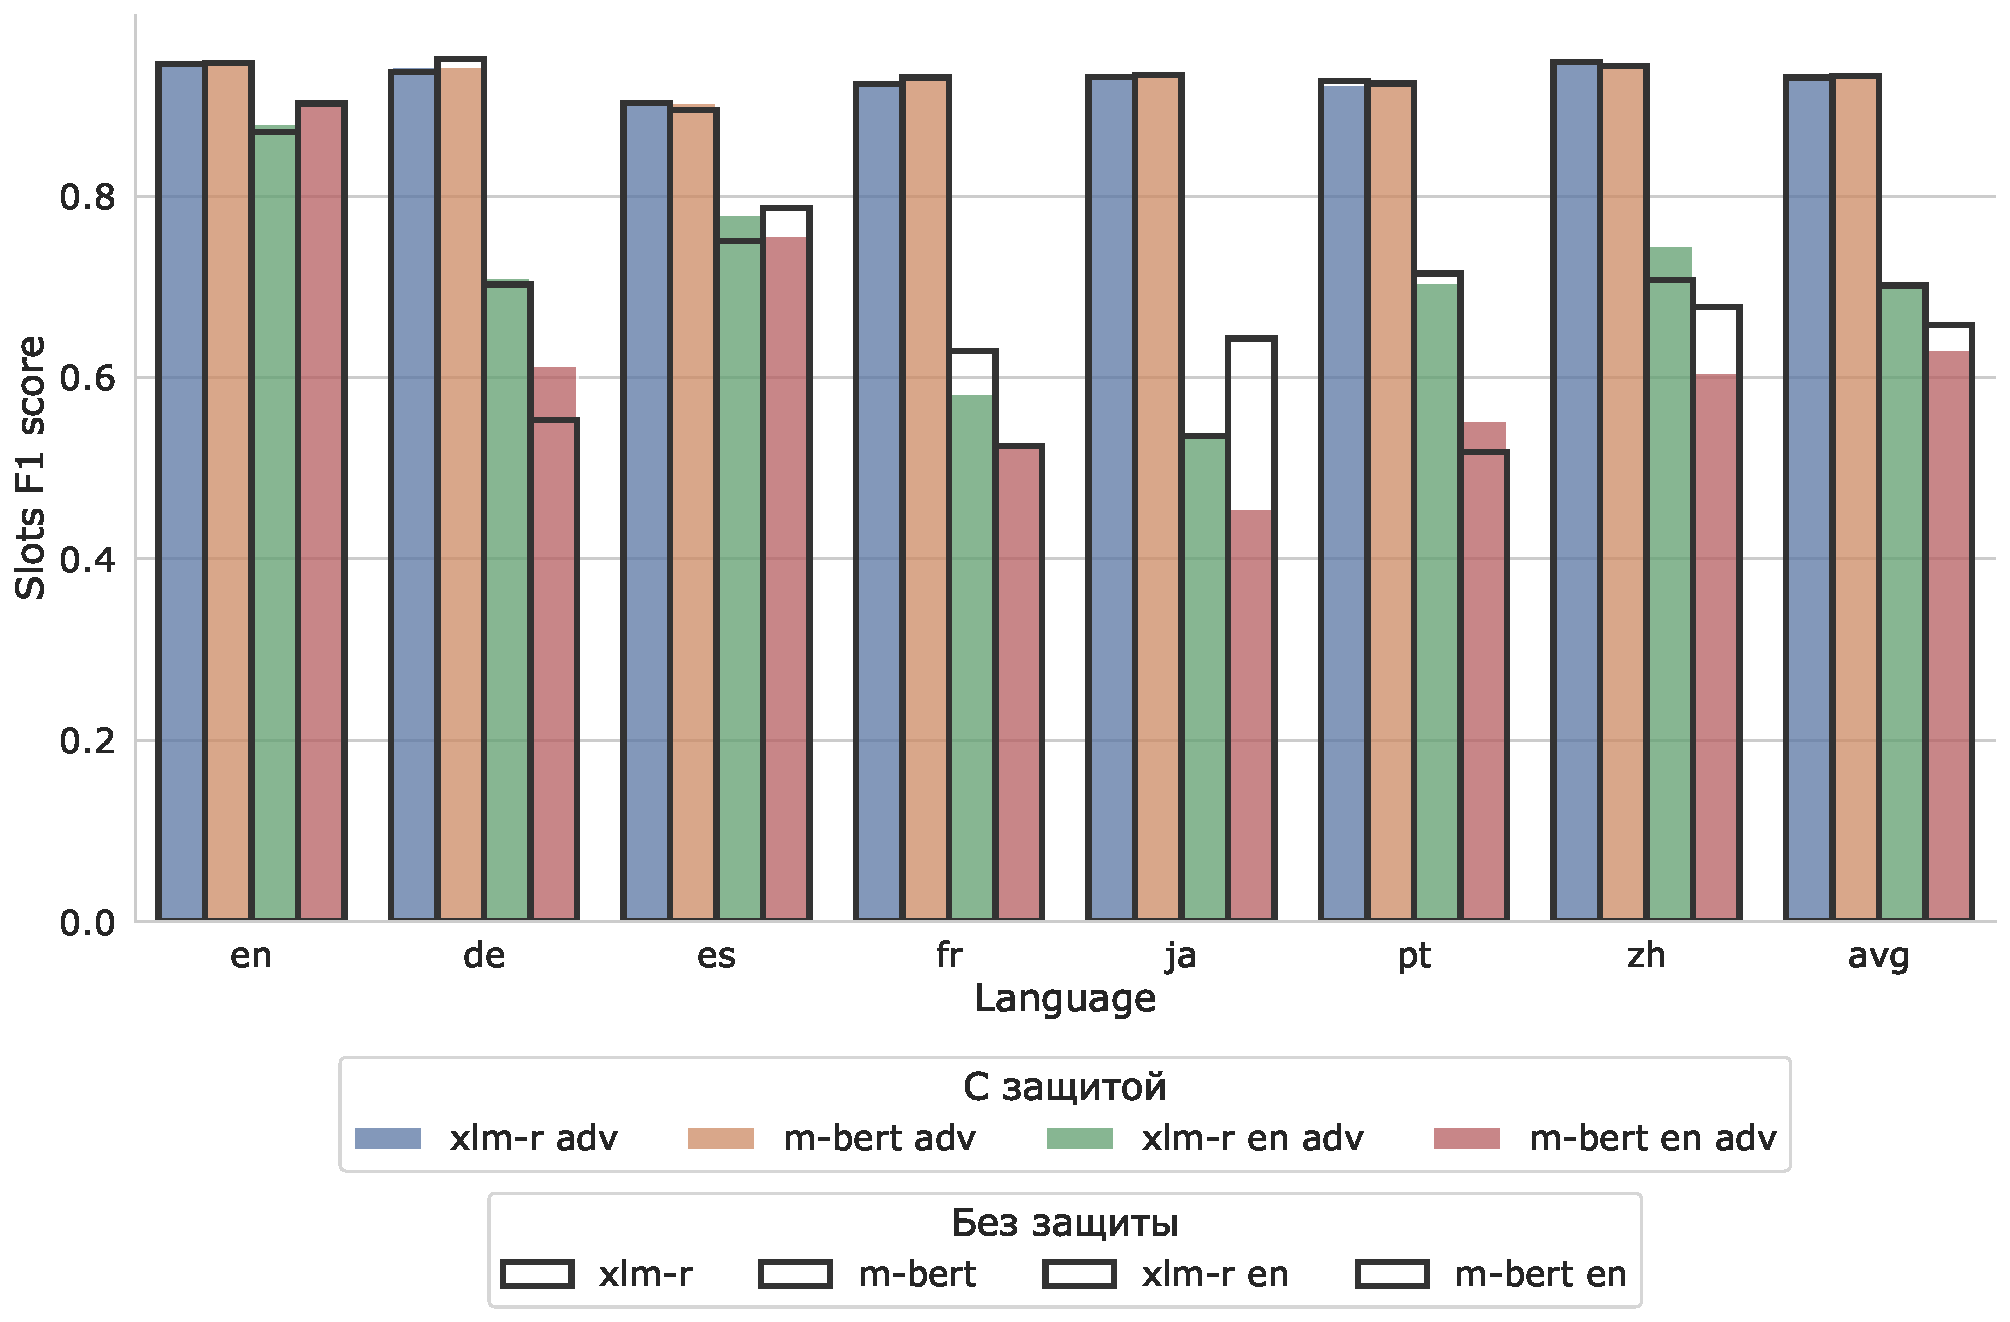
\includegraphics[width=0.9\linewidth]{images/10}\label{fig:figure20}\caption*{F1 мера по слотам}
			\end{figure}
		\end{onlyenv}

		\begin{onlyenv}<3>
			\begin{figure}
				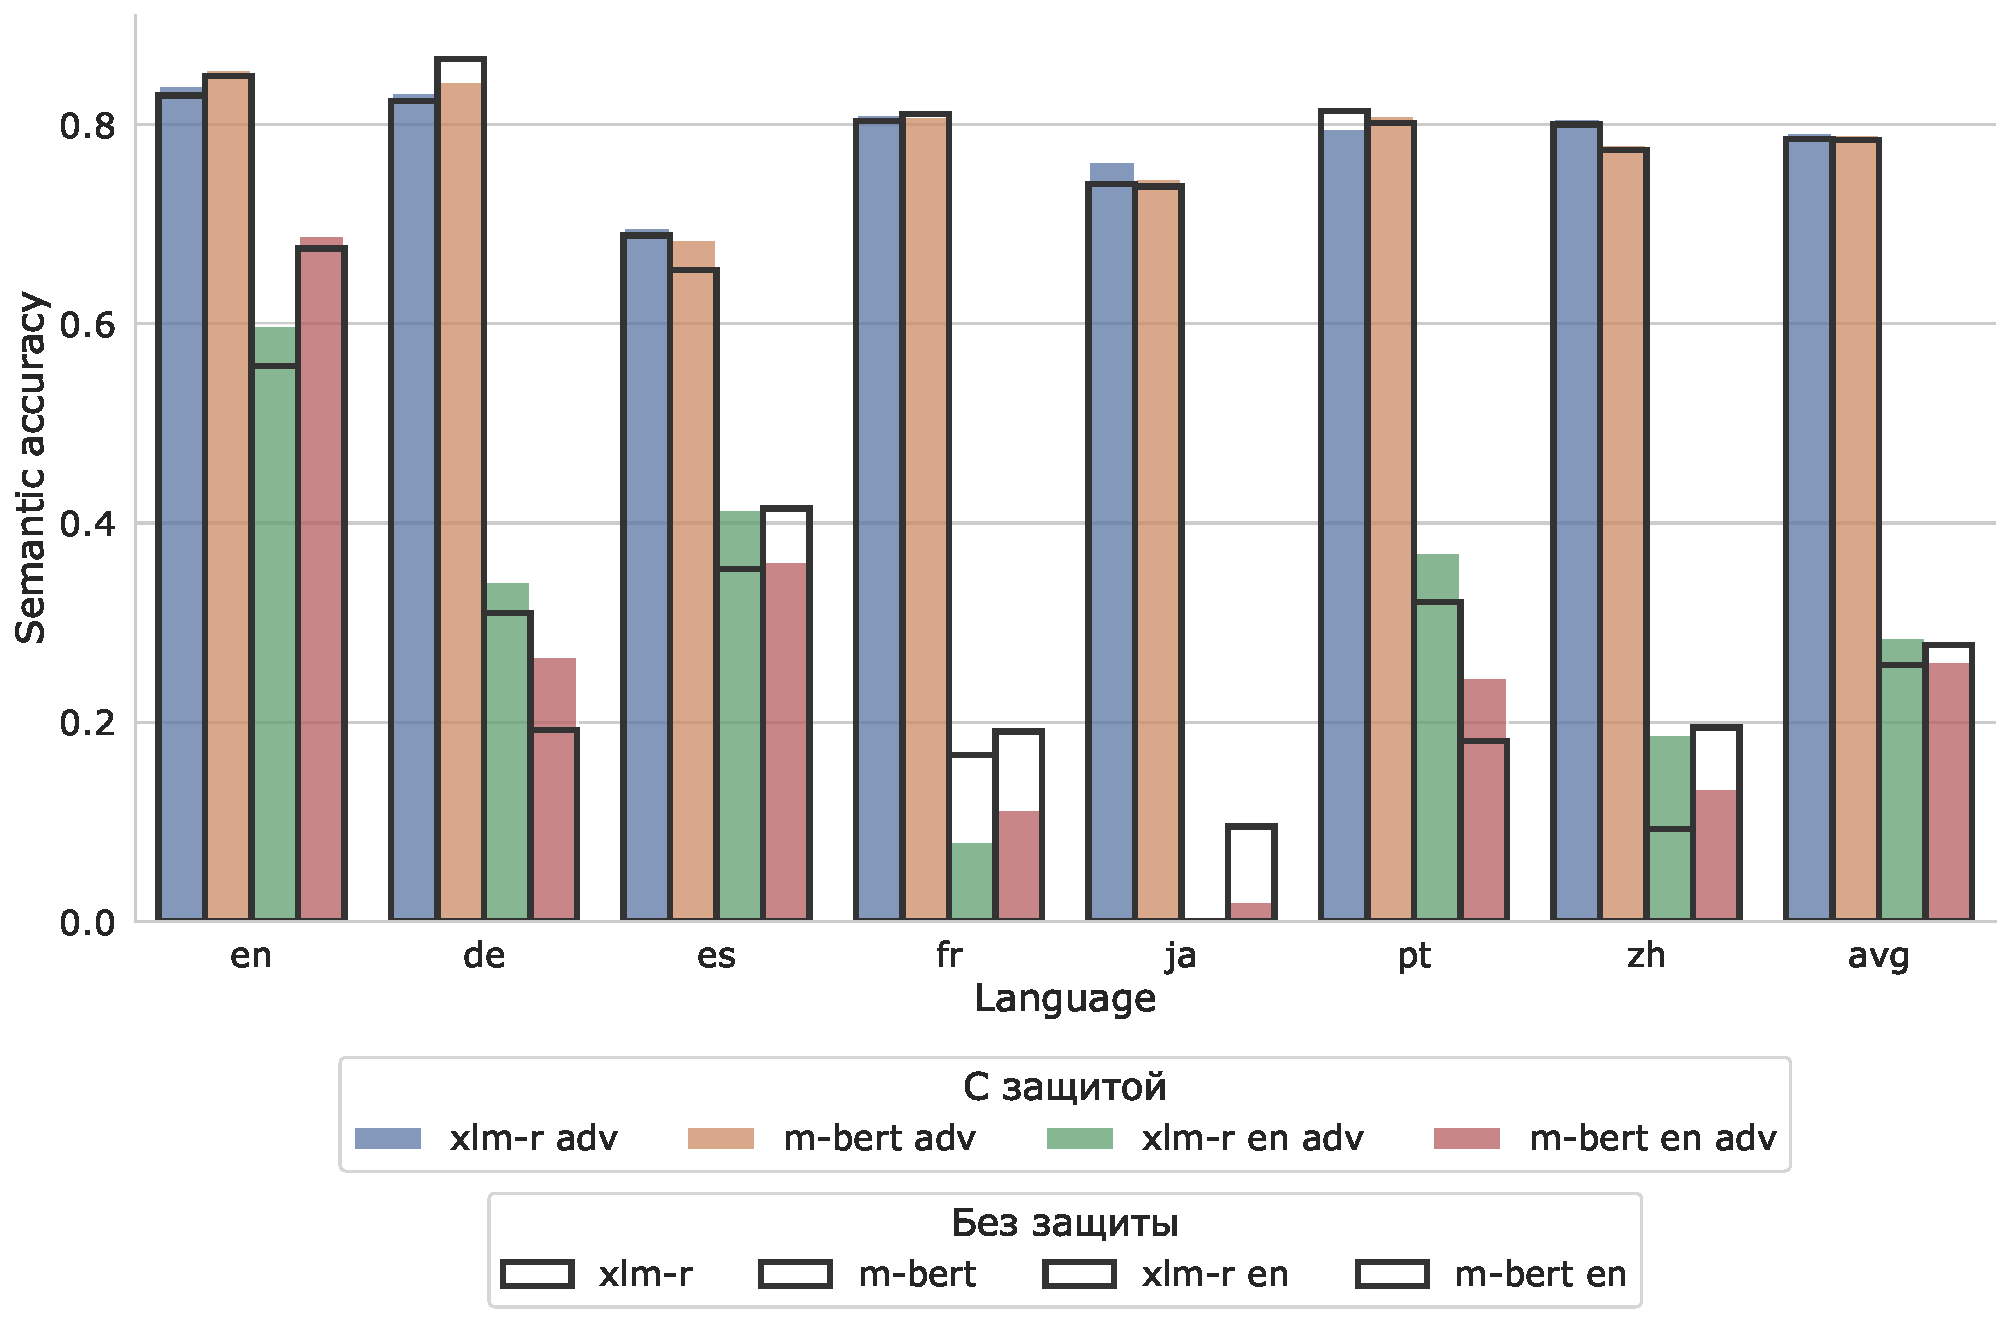
\includegraphics[width=0.9\linewidth]{images/11}\label{fig:figure21}\caption*{Доля полностью верно классифицированных предложений}
			\end{figure}
		\end{onlyenv}

		\note{Мы попробовали защитить модели от наших атак. Для этого мы дообучили тела для обеих моделей и загрузили их перед обучением для задачи классификации интентов и заполнения слотов. Мы обнаружили, что защита почти не повлияла на сильные модели в плане качества на тестовой выборке. Для слабых же моделей эффект на тестовой выборке неоднозначный - качество по интентам упало для азиатских языков, но немного выросло для всех остальных. По слотам же можно говорить о негативном эффекте для модели m-bert, и о позитивном эффекте для модели xlm-r.}
	\end{frame}

	\begin{frame}{Word-level атака (с защитой)}
		\begin{onlyenv}<1>
			\begin{figure}
				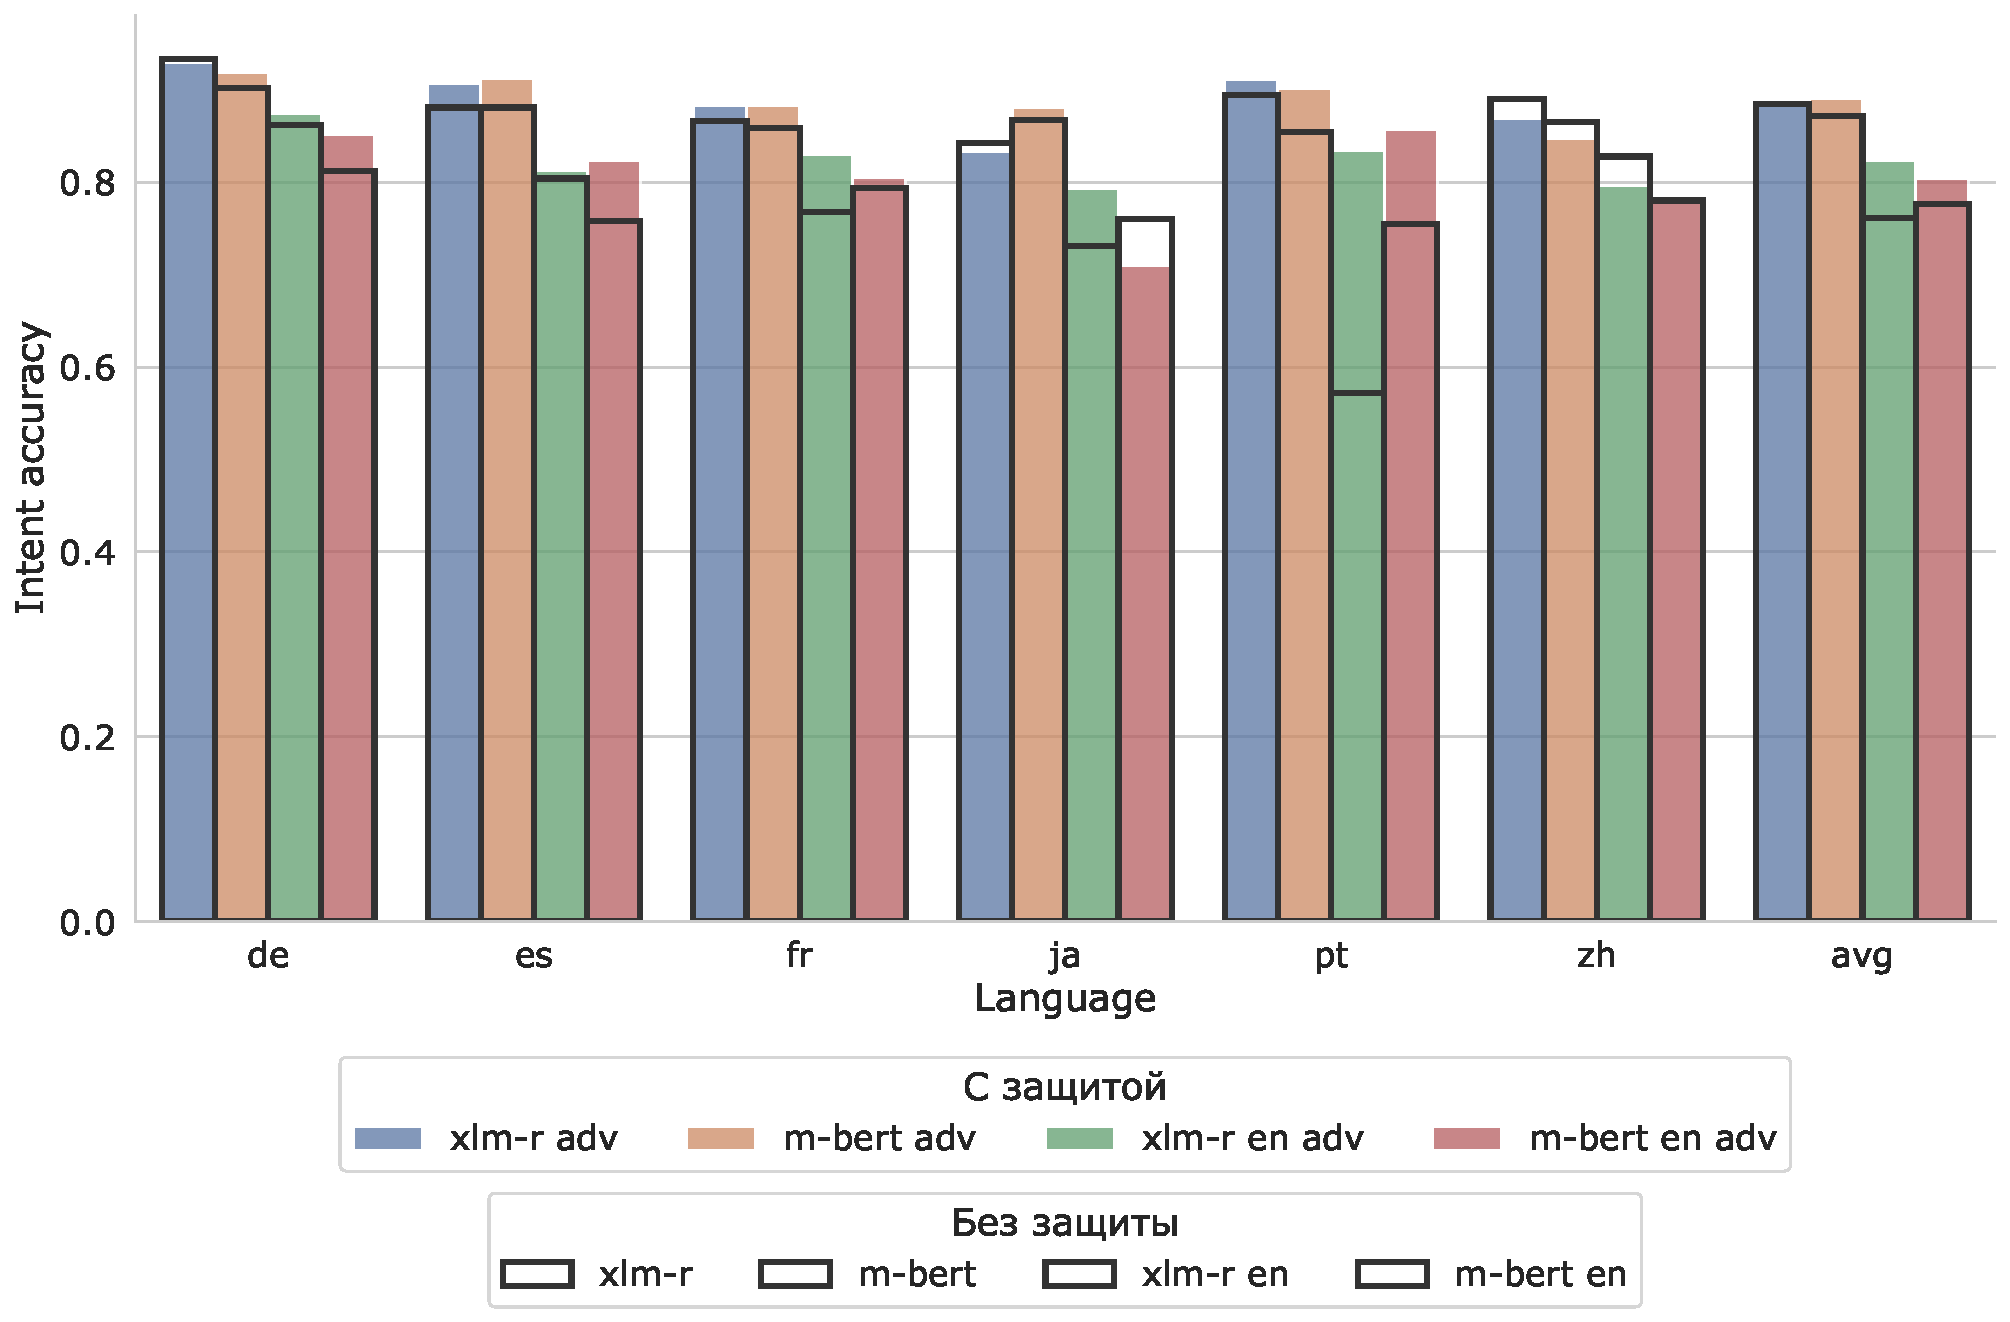
\includegraphics[width=0.9\linewidth]{images/12}\label{fig:figure22}\caption*{Доля предложений с верно классифицированным интентом}
			\end{figure}
		\end{onlyenv}

		\begin{onlyenv}<2>
			\begin{figure}
				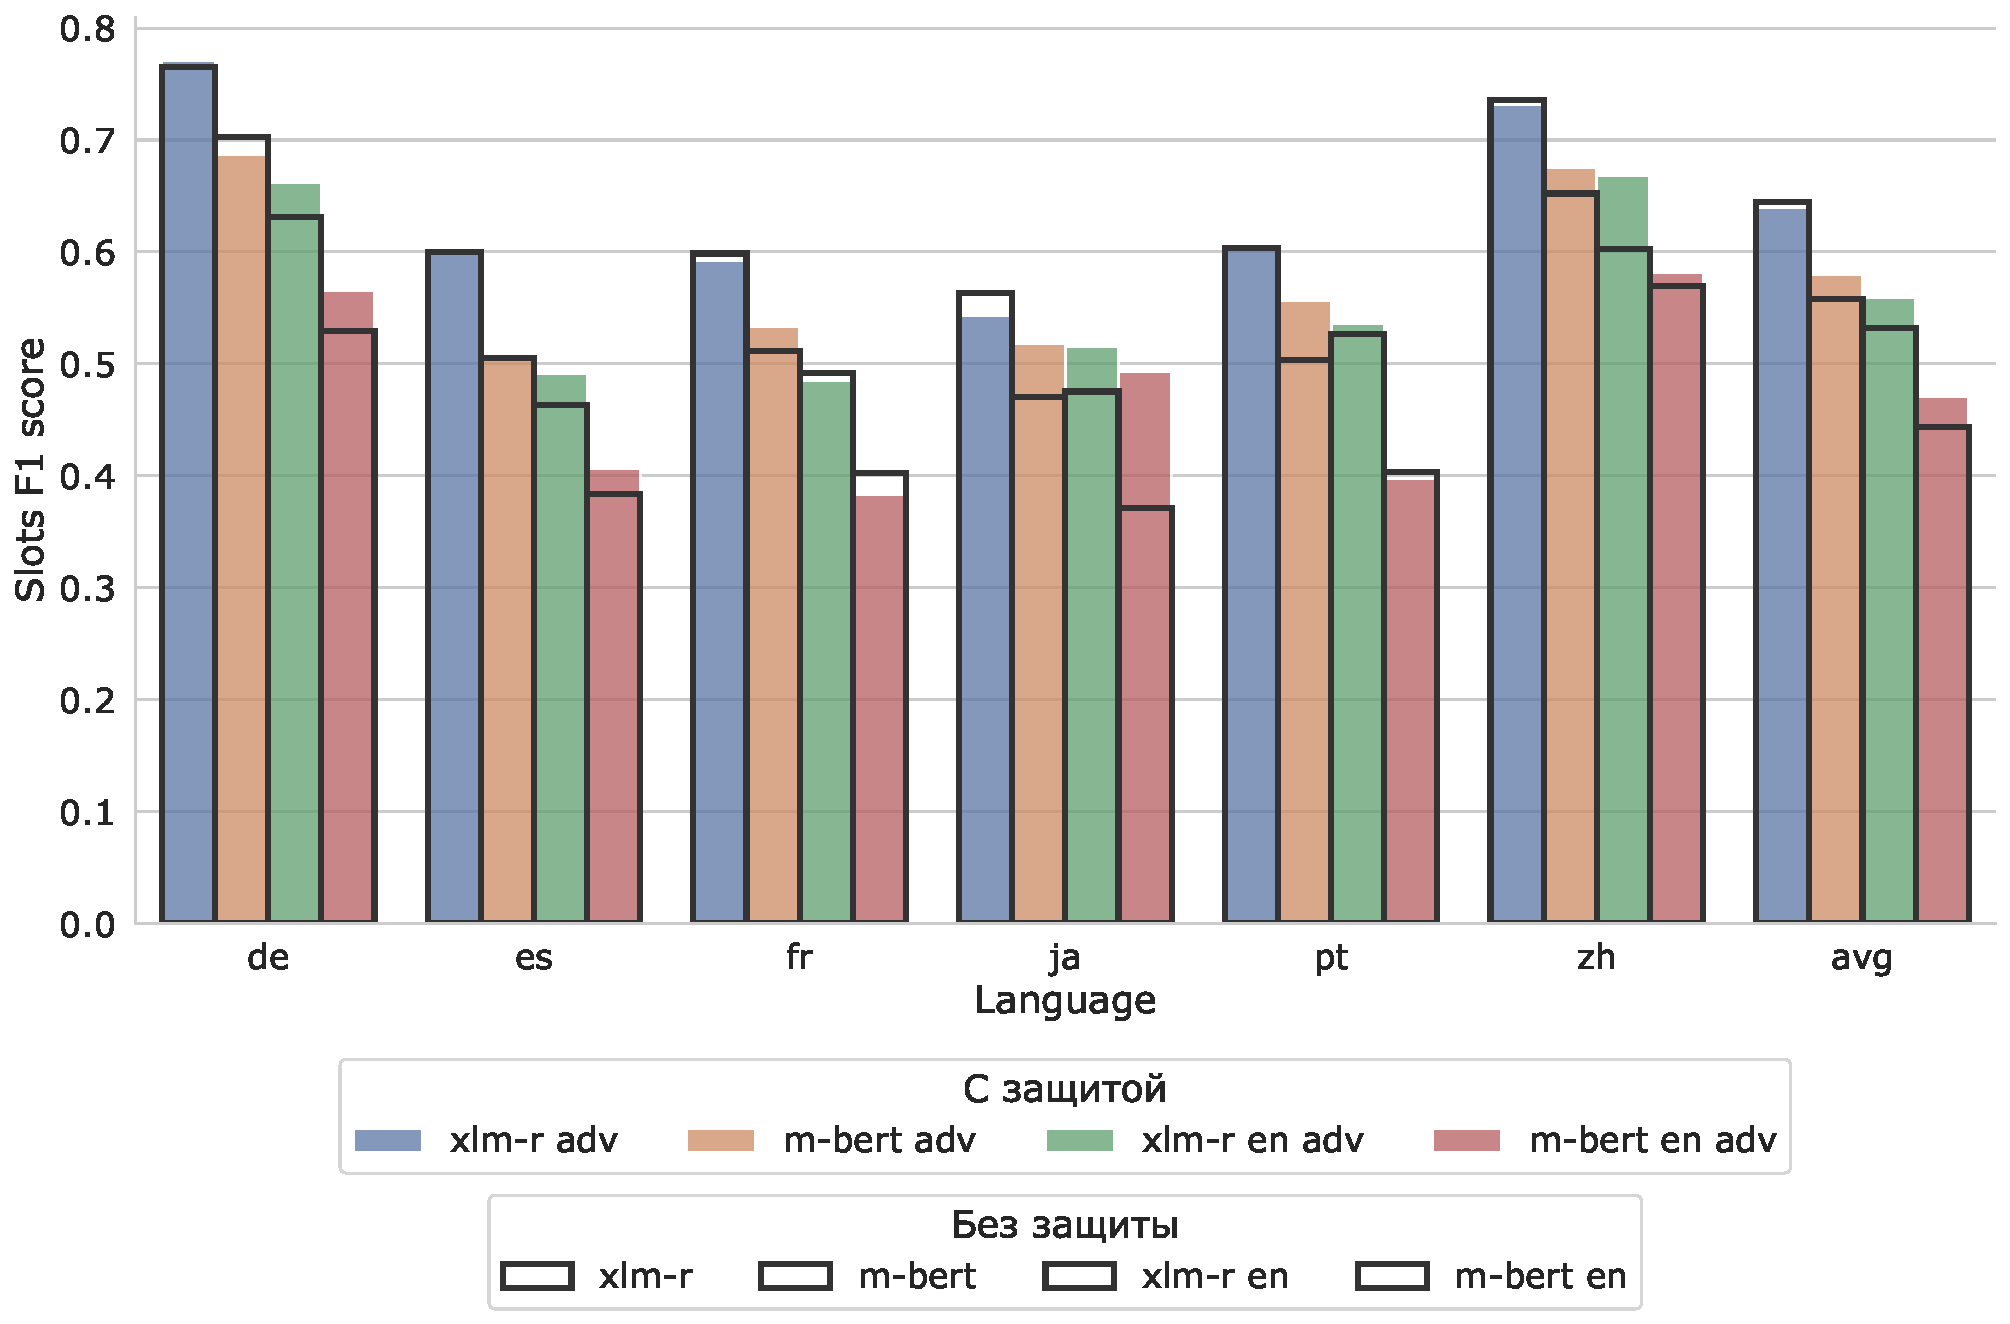
\includegraphics[width=0.9\linewidth]{images/13}\label{fig:figure23}\caption*{F1 мера по слотам}
			\end{figure}
		\end{onlyenv}

		\begin{onlyenv}<3>
			\begin{figure}
				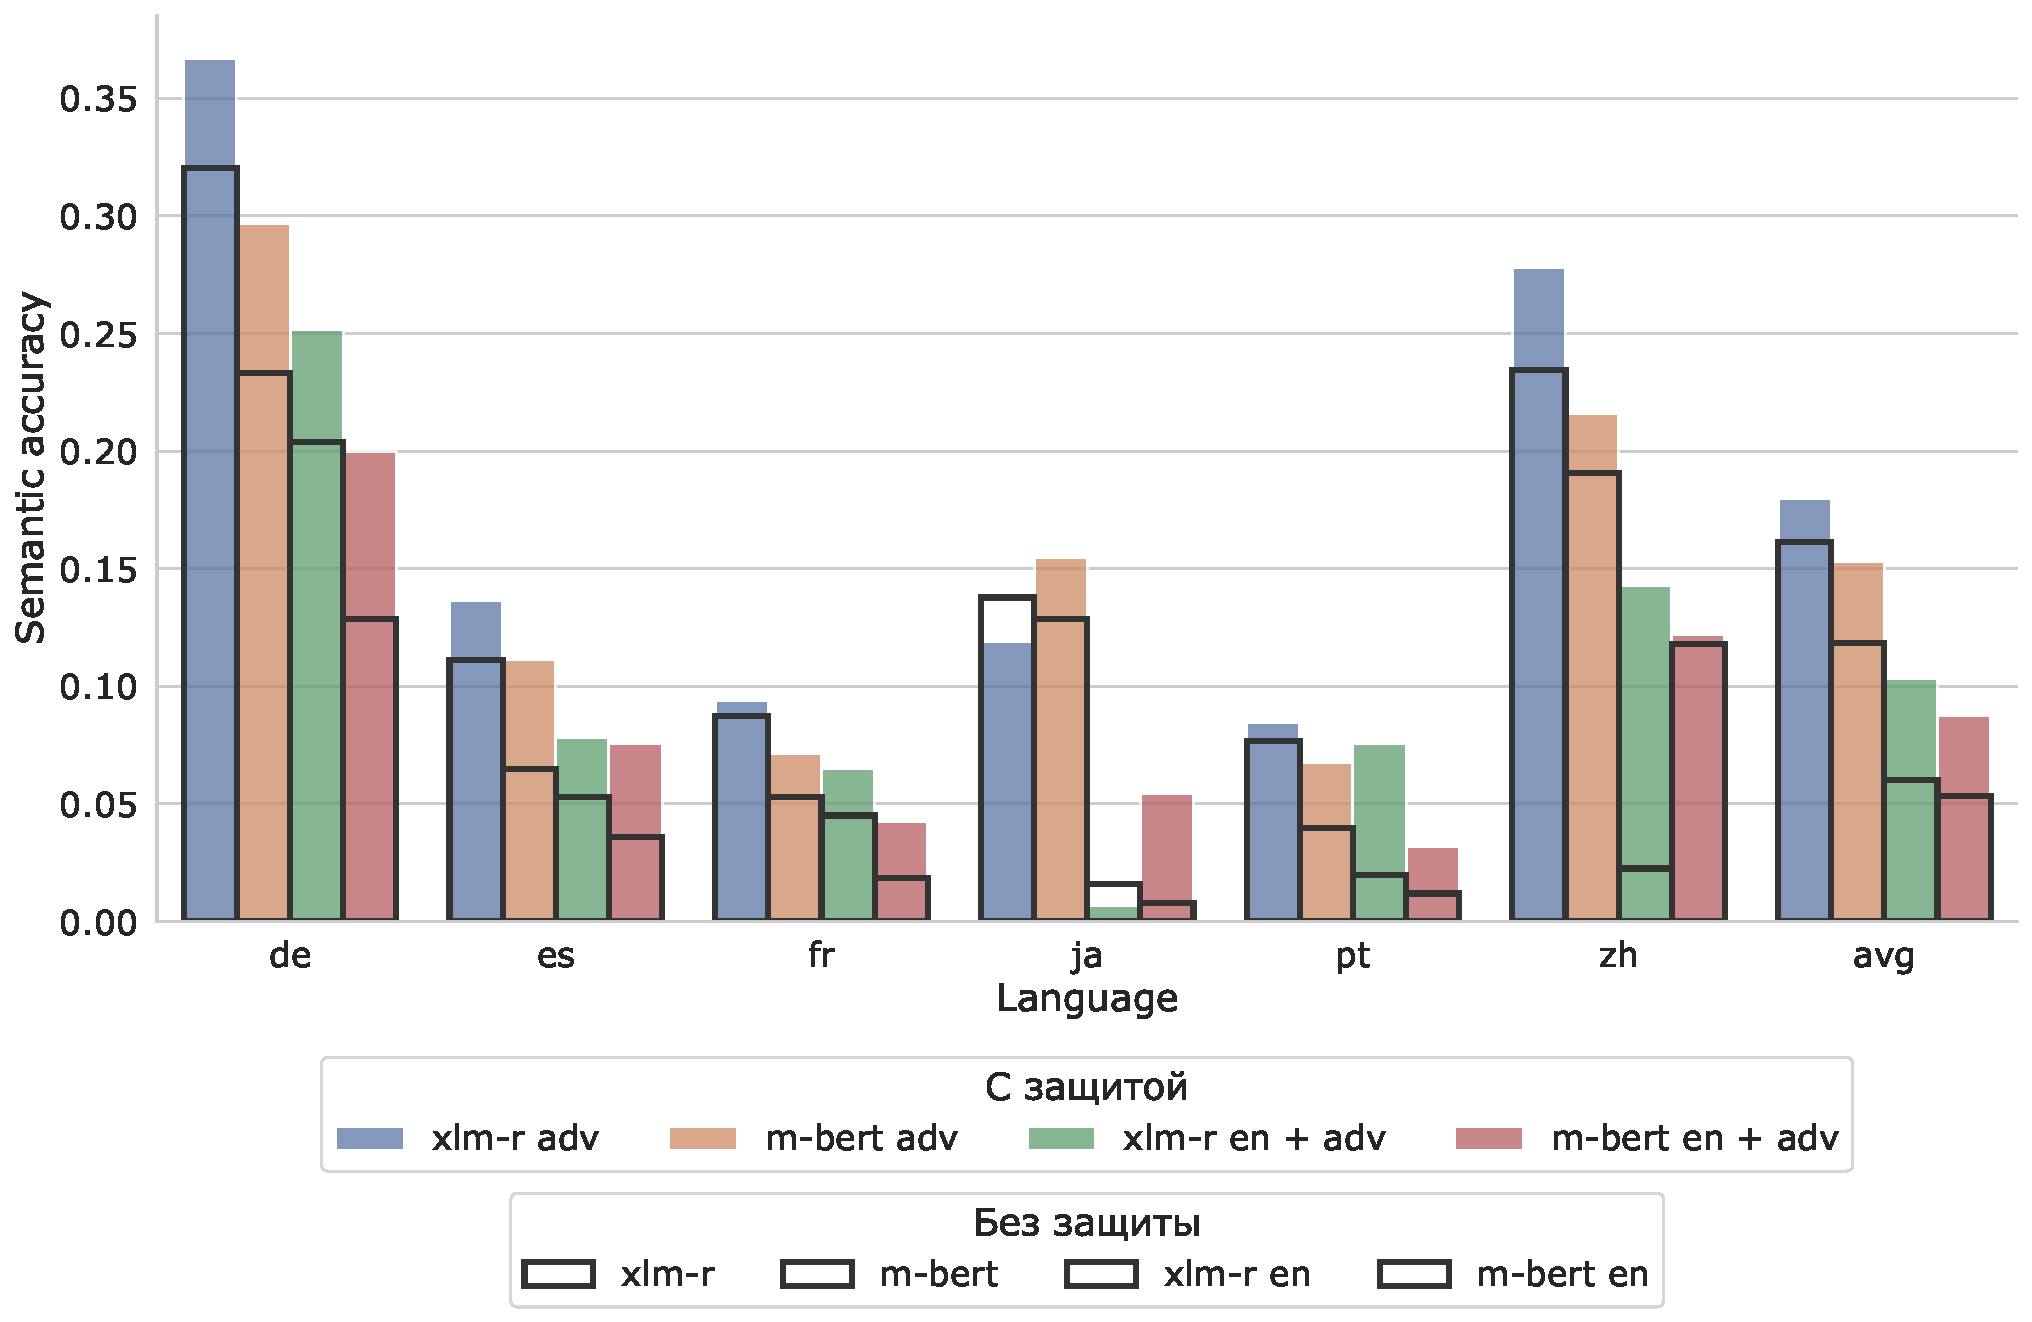
\includegraphics[width=0.9\linewidth]{images/14}\label{fig:figure24}\caption*{Доля полностью верно классифицированных предложений}
			\end{figure}
		\end{onlyenv}

		\note{Для word-level атаки заметно небольшое ухудшение качества по интентам для азиатских языков, и позитивный эффект для остальных языков. После защиты качество по слотам выросло для всех моделей, что в конечном итоге результирует в почти двукратном увеличении доли полностью верно классифицированных предложений для слабых моделей и около 15\% относительного улучшения для сильных моделей}
	\end{frame}

	\begin{frame}{Phrase-level атака (с защитой)}
		\begin{onlyenv}<1>
			\begin{figure}
				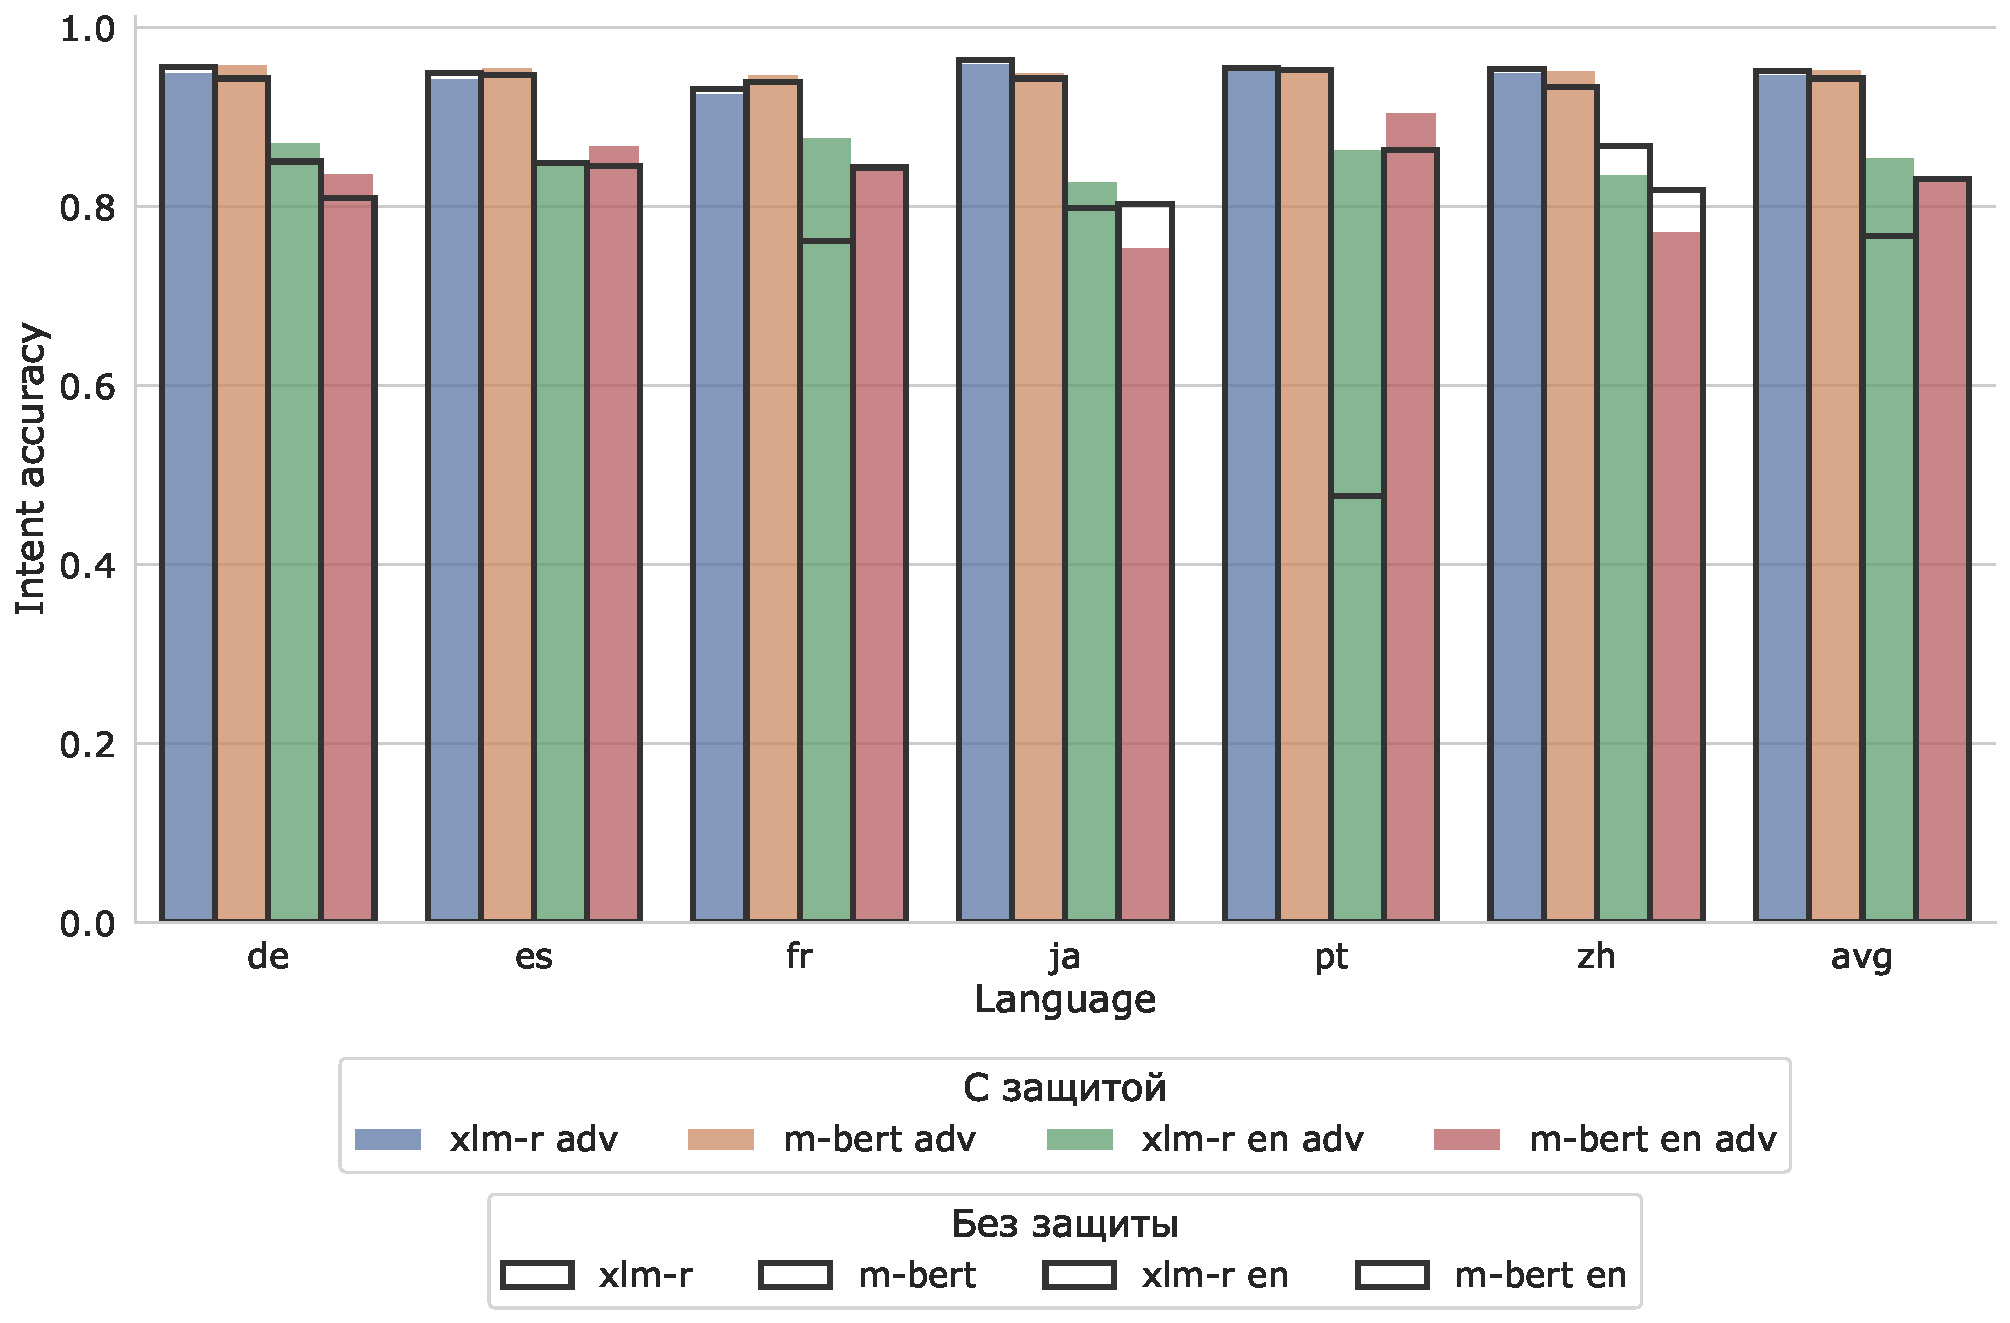
\includegraphics[width=0.9\linewidth]{images/15}\label{fig:figure25}\caption*{Доля предложений с верно классифицированным интентом}
			\end{figure}
		\end{onlyenv}

		\begin{onlyenv}<2>
			\begin{figure}
				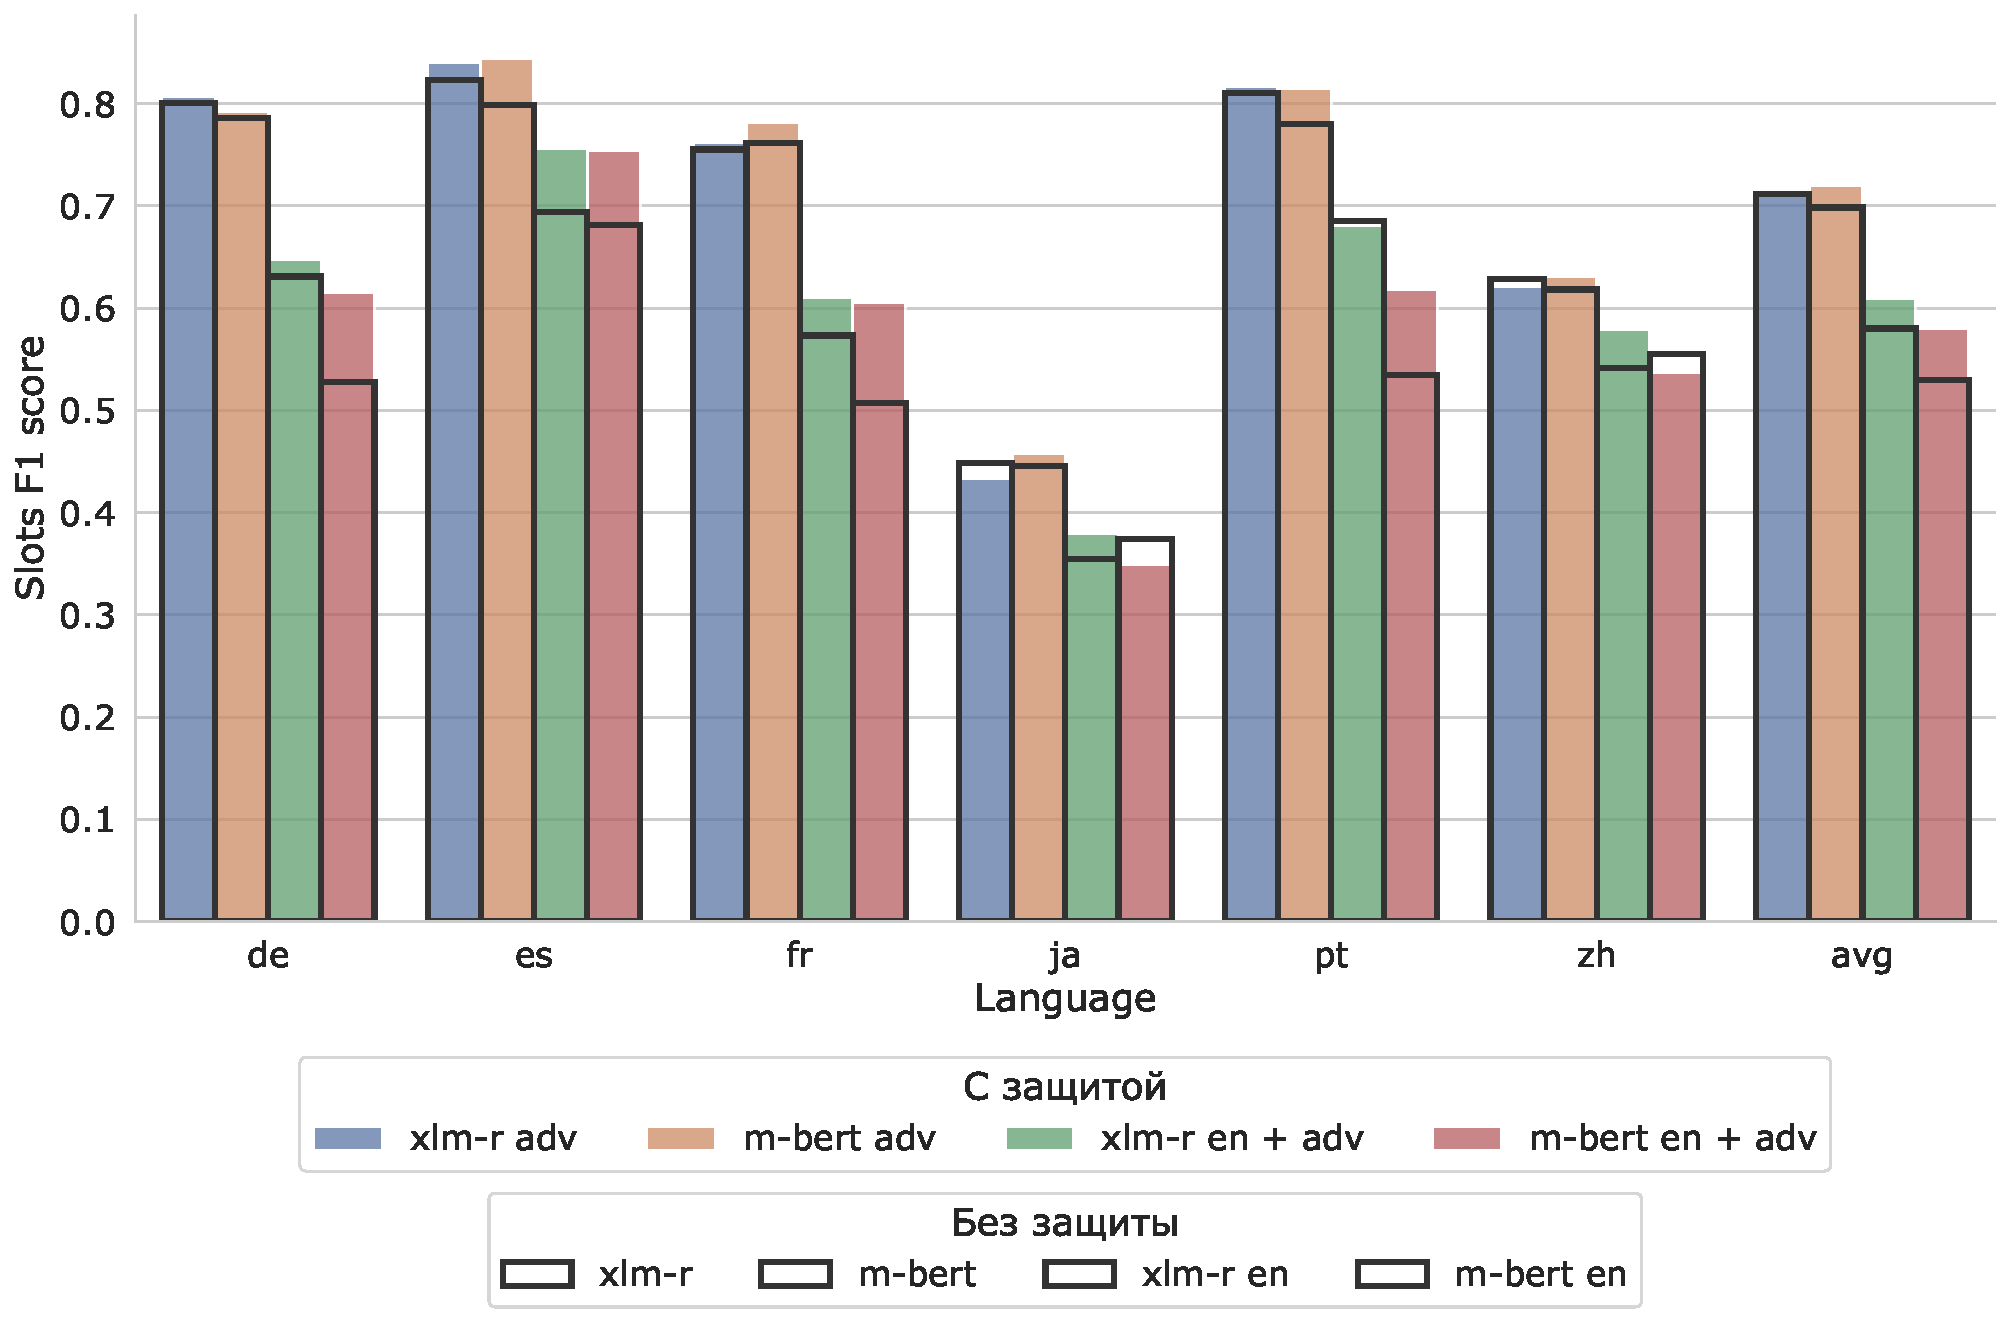
\includegraphics[width=0.9\linewidth]{images/16}\label{fig:figure26}\caption*{F1 мера по слотам}
			\end{figure}
		\end{onlyenv}

		\begin{onlyenv}<3>
			\begin{figure}
				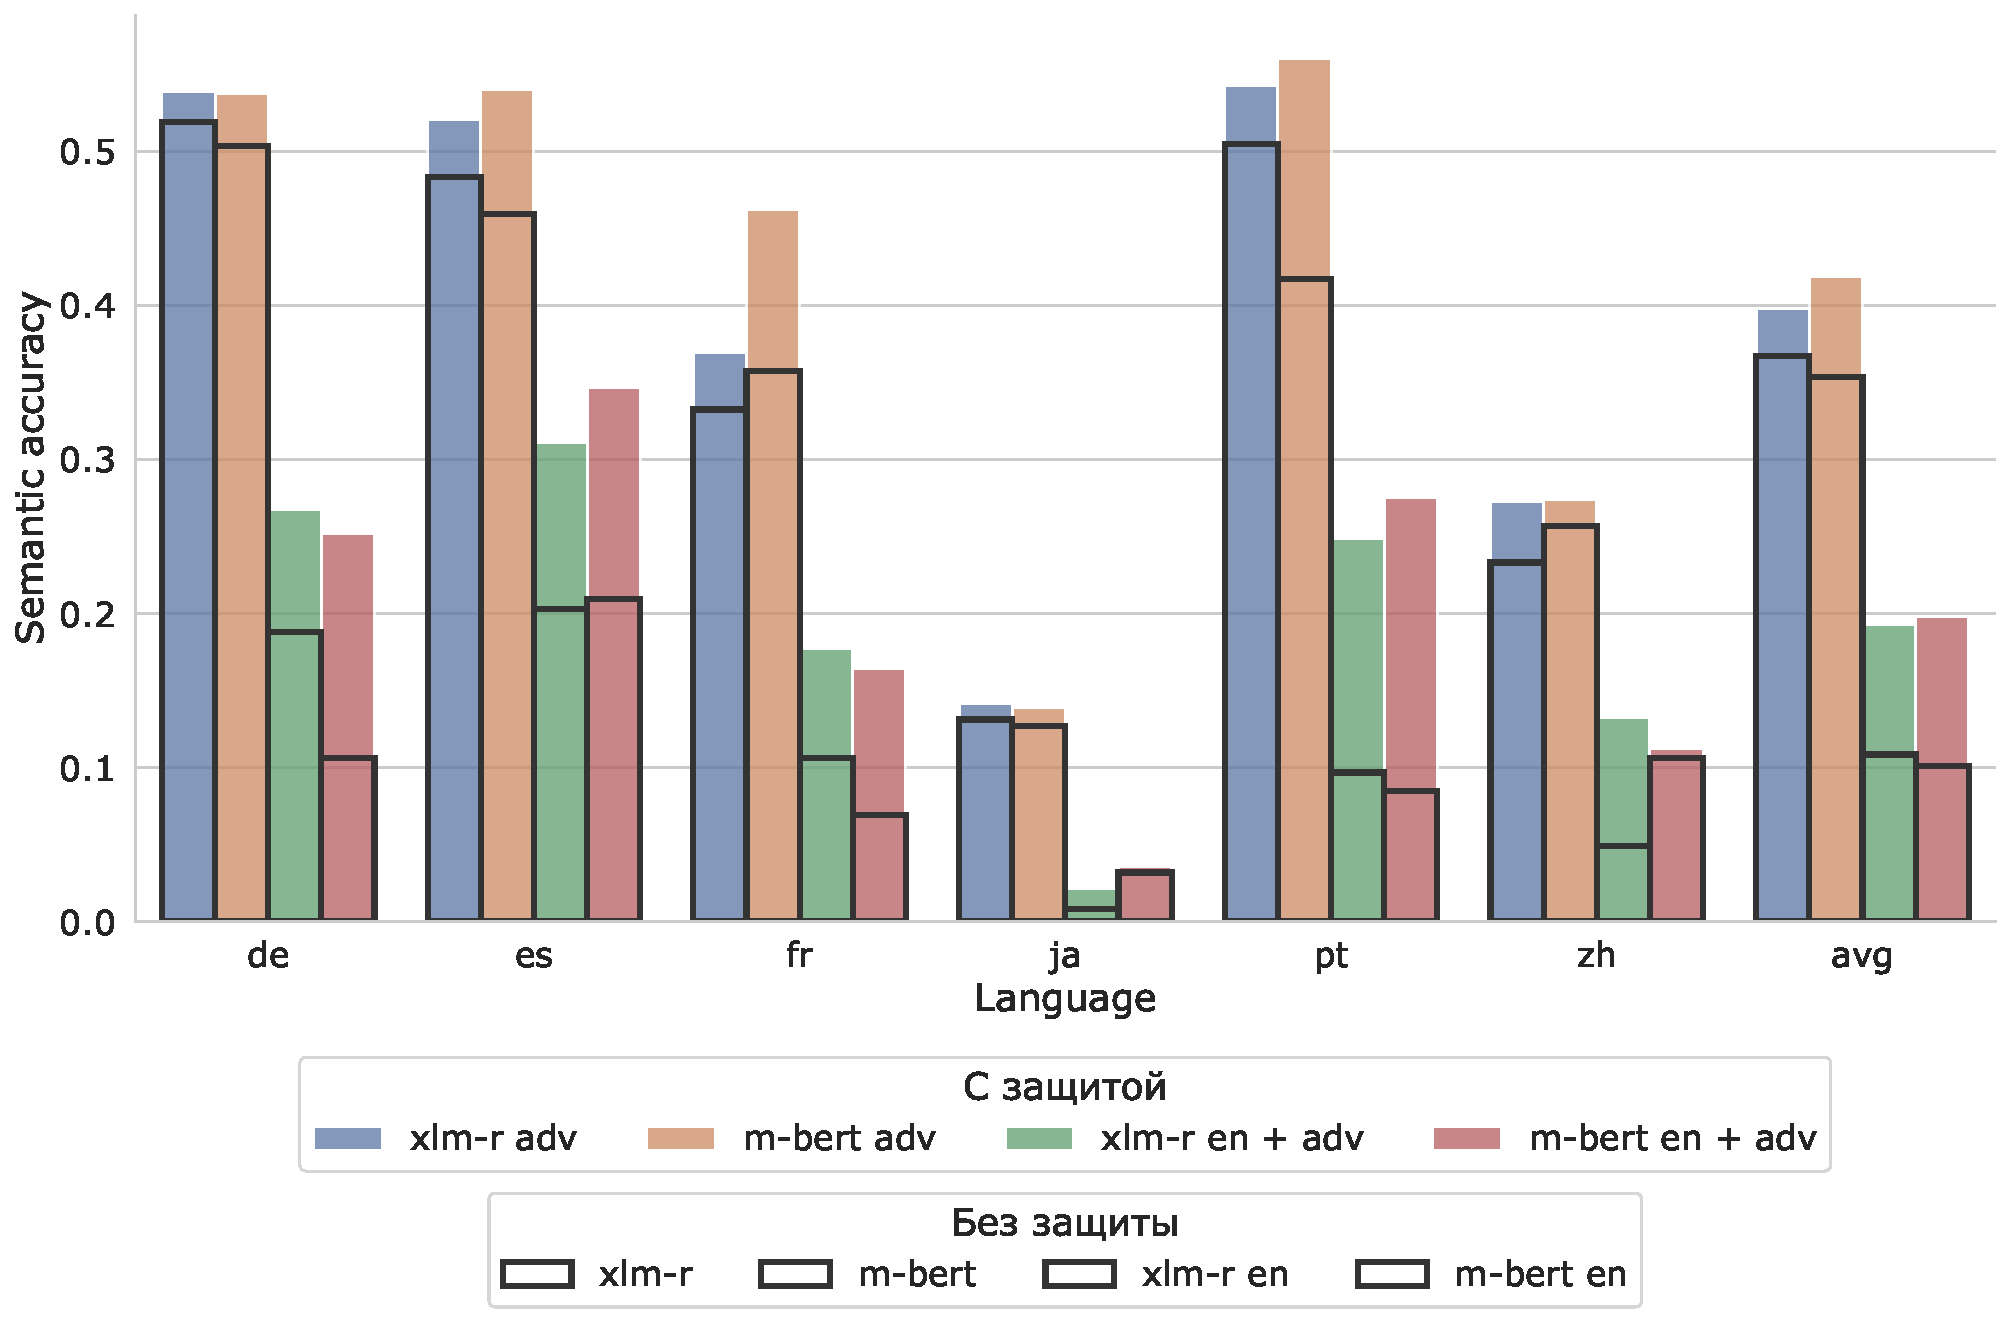
\includegraphics[width=0.9\linewidth]{images/17}\label{fig:figure27}\caption*{Доля полностью верно классифицированных предложений}
			\end{figure}
		\end{onlyenv}

		\note{Для phrase-level атаки опять же заметно небольшое ухудшение качества по интентам для азиатских языков, и позитивный эффект для остальных языков. После защиты качество по слотам немного упало для азиатских языков, и значительно выросло для остальных. Это результирует в двукратном увеличении доли полностью верно классифицированных предложений для слабых моделей и около опять же 15\% относительного улучшения для сильных моделей.}
	\end{frame}

%------------------------------------------------


	\section{Заключение}
%------------------------------------------------

	\begin{frame}
		\frametitle{Заключение}
		\begin{itemize}
			\item<1->Решили задачу классификации интентов и заполнения слотов
			\item<2->Провели анализ качества моделей после двух предложенных атак
			\item<3->Провели анализ качества моделей после предложенного метода защиты
		\end{itemize}

		\note{В итоге, в своей работе мы решили задачу классификации интентов и заполнения слотов. Мы провели исследование влияния смешения кодов на две мультиязычные языковые модели XLM-RoBERTa и m-BERT. Мы провели анализ с помощью двух атак по методу серого ящика и показали, что смешение кодов может стать заметной проблемой при применении языковых моделей на практике. Однако, предложенный нами метод защиты показывает хорошие результаты и помогает улучшить качество после атаки.\newlineВ качестве дальнейшей работы мы рассматриваем анализ других мультиязычных моделей, построение новых более реалистичных атак, имитирующих смешение кодов и поиск новых алгоритмов защиты от подобных атак.}
	\end{frame}

	\begin{frame}
		\centerСпасибо за внимание!
		\note{Спасибо за внимание!}
	\end{frame}

	\begin{frame}
		\printbibliography
	\end{frame}

\end{document}
